\documentclass[11pt,twocolumn]{article}

% ------------------------------------------------------------------ layout
\usepackage[a4paper,margin=1.8cm]{geometry}
\setlength{\columnsep}{18pt}
\setlength{\emergencystretch}{2em}
\usepackage[expansion=false]{microtype} % expansion needs scalable fonts absent here (cf. T1 note)
%\usepackage[T1]{fontenc} % cm-super absent; OT1 Type-1 CM keeps fonts scalable
\usepackage[utf8]{inputenc}

% ------------------------------------------------------------------- maths
\usepackage{amsmath,amssymb,amsthm,mathtools,bm}
\usepackage{siunitx}

% ------------------------------------------------------------------ floats
\usepackage{graphicx}
\usepackage{booktabs}
\usepackage{multirow}
\usepackage{array}
\usepackage{caption}
\usepackage{subcaption}
\usepackage{longtable}
\usepackage{tabularx}
\captionsetup{font=small,labelfont=bf}

% ---------------------------------------------------------------- algorithms
\usepackage{algorithm}
\usepackage{algpseudocode}

% ------------------------------------------------------------------- code
\usepackage{listings}
\usepackage{xcolor}
\definecolor{codegray}{gray}{0.45}
\definecolor{codebg}{gray}{0.97}
\lstset{
  language=Python,
  basicstyle=\ttfamily\footnotesize,
  commentstyle=\color{codegray}\itshape,
  keywordstyle=\bfseries,
  stringstyle=\color{codegray},
  showstringspaces=false,
  numbers=left,
  numberstyle=\tiny\color{codegray},
  numbersep=8pt,
  breaklines=true,
  breakatwhitespace=true,
  frame=single,
  rulecolor=\color{black!25},
  backgroundcolor=\color{codebg},
  captionpos=b,
  aboveskip=1.0\baselineskip,
  belowskip=1.0\baselineskip
}

% ------------------------------------------------------------------- TikZ
\usepackage{tikz}
\usetikzlibrary{arrows.meta,positioning,fit,calc,shapes.geometric}
\tikzset{
  block/.style={draw, rounded corners=2pt, minimum height=9mm, minimum width=22mm, align=center, font=\small},
  qblock/.style={block, fill=black!6},
  arrow/.style={-{Latex[length=2.4mm]}, thick}
}

% ------------------------------------------------------------- references
\usepackage{cuted}          % full-width in-place blocks (strip) across both columns
\makeatletter\providecommand{\@setmarks}{}\makeatother % cuted's \@outputdblcol calls \@setmarks, absent in this kernel
\renewcommand{\dbltopfraction}{0.92}
\renewcommand{\dblfloatpagefraction}{0.75}
\renewcommand{\textfraction}{0.06}
\setcounter{dbltopnumber}{4}
\usepackage[numbers,sort&compress]{natbib}
\usepackage[hidelinks]{hyperref}

% ------------------------------------------------------------ environments
\newtheorem{definition}{Definition}[section]
\newtheorem{proposition}{Proposition}[section]
\newtheorem{remark}{Remark}[section]

% ---------------------------------------------------------------- notation
\newcommand{\R}{\mathbb{R}}
\newcommand{\C}{\mathbb{C}}
\newcommand{\Hil}{\mathcal{H}}
\newcommand{\tr}{\operatorname{Tr}}
\newcommand{\id}{\mathbb{1}}
\newcommand{\map}[1]{\mathcal{#1}}
\newcommand{\ket}[1]{|#1\rangle}
\newcommand{\bra}[1]{\langle#1|}
\newcommand{\braket}[2]{\langle#1|#2\rangle}
\newcommand{\ketbra}[2]{|#1\rangle\!\langle#2|}
\newcommand{\ev}[1]{\langle #1\rangle}
\newcommand{\code}[1]{\texttt{#1}}
\newcommand{\NMSE}{\mathrm{NMSE}}

\newcommand{\parttitle}[2]{%
  \twocolumn[{%
    \phantomsection
    \addcontentsline{toc}{section}{\texorpdfstring{\textbf{Part #1.\ #2}}{Part #1. #2}}%
    \begin{center}
      {\Large\bfseries Part #1}\\[2mm]
      {\LARGE\bfseries #2}
    \end{center}
    \vspace{4mm}%
  }]%
}

\setcounter{tocdepth}{2}
\setcounter{secnumdepth}{3}

\title{\bfseries Quantum Reservoir Computing for Renewable Energy and Climate Prediction:\\[2mm]
\Large A Research Review and Implementation Handbook}
\author{Prepared for Quantathon 2026}
\date{3 July 2026; revised 11 July 2026 (Parts IX--XI added)}

\begin{document}

\maketitle
\onecolumn
\begin{abstract}
\noindent
Quantum reservoir computing (QRC) trains only a linear read-out on the measured
observables of a fixed, input-driven quantum system, sidestepping the trainability
problems of variational quantum circuits while inheriting the temporal-processing
strengths of classical reservoir computing. Renewable-energy and climate time
series --- solar irradiance, wind power, electric load, and coupled ocean--atmosphere
indices --- are a natural application domain: they are abundantly available, exhibit
memory and nonlinearity on many time scales, and support an economically important
forecasting industry against which any quantum claim can be honestly benchmarked.
This document is both a formal research review and an implementation handbook. It
develops classical reservoir computing and its guarantees (echo-state property,
fading memory, universality); formulates QRC in the language of quantum channels
and derives where nonlinearity, memory, and measurement enter; surveys the
principal reservoir architectures and hardware platforms; provides complete,
line-by-line-explained implementations in Cirq, Qiskit, and PennyLane, including
transpilation to native gate sets, realistic noise, finite-shot estimation, and
mid-circuit measurement with reset; catalogues and analyses public renewable-energy
and climate datasets with full exploratory data analysis of three of them; assembles
end-to-end forecasting pipelines that share one mathematical structure across
frameworks; and closes with design principles and ten concrete research directions.
All numerical results in this document were produced by the code shipped alongside
it, every experiment reports size-matched classical baselines and structureless
quantum controls, and no claim of quantum advantage is made where none was observed.
\end{abstract}

\vspace{2mm}
\subsection*{How to read this document}

Parts~I and~II build the theory in a linear order and are prerequisites for
everything else. Part~III (architectures) and Part~V (hardware) are reference
material: they can be read selectively. Part~IV is the software handbook and is
best read at a keyboard, alongside the \code{code/} directory that ships with
this document. Part~VI introduces the application domain and its data; Part~VII
assembles the pieces into complete pipelines; Part~VIII distils design judgement
and proposes research programmes. A reader who already knows classical reservoir
computing can start at Part~II; a reader who wants to forecast something by
tonight can start at Part~VII and backtrack as needed. Parts~IX--XI, added in
the July 2026 revision, are forward-looking: Part~IX designs the staged
repository that consolidates this document's code with the qubit-reuse
compiler, Part~X gives the theory and pre-registered implementation plan for
the recurrence-free reservoir with virtual-node readout, and Part~XI wraps
the forecast core in a full product pipeline with a survey of classical
ML/DL and agentic-AI post-processing.

\subsection*{Epistemic conventions}

Three kinds of statement appear in this document and are kept explicitly
distinct. \emph{Theory} means a mathematical statement with stated assumptions,
attributed to the literature or derived in the text. \emph{Simulation} means a
numerical result produced by the exact density-matrix or statevector code in
\code{code/}, on either synthetic surrogate data (always labelled
\emph{surrogate}) or real recorded data (always labelled \emph{real}).
\emph{Hardware} means a result reported in the literature from a physical
quantum device; this document runs no hardware jobs itself, but Part~IV's Qiskit
pipeline is written exactly as a hardware submission would be, including
transpilation, native basis gates, coupling constraints, realistic noise, and
finite shots. Throughout, reported errors are normalised mean-square errors
(NMSE), for which predicting the training-set mean scores $1.0$; any method
worth attention must sit well below that line, and every figure that shows an
NMSE also shows it.

\clearpage
\tableofcontents

\clearpage
\section*{Notation}
\addcontentsline{toc}{section}{Notation}

\begin{center}
\small
\begin{tabular}{@{}ll@{}}
\toprule
Symbol & Meaning \\
\midrule
$u_t \in \R^{d_{\mathrm{in}}}$ & input at discrete time $t$ (scalar unless stated) \\
$y_t$, $\hat y_t$ & target and predicted output \\
$x_t \in \R^{N_x}$ & classical reservoir state / extracted feature vector \\
$W_{\mathrm{res}}, W_{\mathrm{in}}, b$ & fixed reservoir, input, and bias weights \\
$W_{\mathrm{out}}$ & trained linear read-out \\
$f(\cdot)$ & elementwise activation (typically $\tanh$) \\
$\alpha$ & leak rate of a leaky-integrator reservoir \\
$\rho_t$ & reservoir density matrix at time $t$ \\
$\Hil$, $d=2^n$ & Hilbert space and its dimension for $n$ qubits \\
$\map{E}_{\theta,u}$ & input-dependent CPTP map (quantum reservoir update) \\
$K_j$ & Kraus operators, $\sum_j K_j^\dagger K_j = \id$ \\
$\map{L}$ & Lindblad generator \\
$O_k$, $x_t^{(k)}=\tr(O_k\rho_t)$ & measured observable and feature \\
$X_i, Y_i, Z_i$ & Pauli operators on qubit $i$ \\
$H$, $J_{ij}$, $h_i$ & Hamiltonian, couplings, fields \\
$\Delta t$ & input injection interval (evolution time per step) \\
$V$ & number of virtual nodes (temporal multiplexing) \\
$S$ & number of measurement shots \\
$L$ (or $W$) & input-window length in restart protocols \\
$\lambda$ & ridge-regression penalty \\
$\mathrm{MC}$, $\mathrm{MC}_d$ & total and delay-$d$ linear memory capacity \\
$\NMSE$ & mean-square error normalised by target variance \\
$\ev{r}$ & mean level-spacing ratio (chaos diagnostic) \\
$T_1$, $T_2$ & energy relaxation and dephasing times \\
\bottomrule
\end{tabular}
\end{center}


\parttitle{I}{Foundations of Classical Reservoir Computing}

\section{The reservoir computing paradigm}
\label{sec:rc-paradigm}

Reservoir computing (RC) is a way of using a fixed dynamical system as a
computational resource. A time-dependent input drives the system; the system's
internal state, by virtue of its own dynamics, becomes a rich nonlinear
function of the input history; and a simple \emph{linear} map from the state to
the output is the only component that is ever trained. The paradigm emerged
twice independently around 2001--2002: as \emph{echo state networks} (ESNs) in
the machine-learning community~\citep{jaeger2001echo,jaeger2004harnessing} and
as \emph{liquid state machines} in computational
neuroscience~\citep{maass2002realtime}; the two were later unified under the
reservoir computing name~\citep{verstraeten2007experimental,lukosevicius2009reservoir}.

The appeal of the paradigm is threefold. First, training is a linear
least-squares problem --- convex, closed-form, and cheap --- so the pathologies of
training recurrent networks by gradient descent (vanishing and exploding
gradients through time) never arise. Second, because the dynamical core is
fixed, \emph{any} sufficiently rich dynamical system can serve as the
reservoir; this is what opens the door to physical and, in this document,
quantum reservoirs. Third, despite the simplicity of training, reservoir
computers are provably universal approximators for an important class of
input--output maps (Section~\ref{sec:universality}) and are competitive in
practice on chaotic time-series prediction, a task family directly relevant to
weather and climate~\citep{pathak2018model,arcomano2020machine,vlachas2020backpropagation}.

Figure~\ref{fig:rc-blocks} fixes the three-layer anatomy used throughout this
document: an \emph{encoding} (input layer), a fixed \emph{reservoir}, and a
trained linear \emph{read-out}. Every architecture in Part~III, quantum or
classical, is an instance of this anatomy; design work happens almost entirely
in the first two layers, and honesty in evaluation happens in the third.

\begin{figure*}[t]
\centering
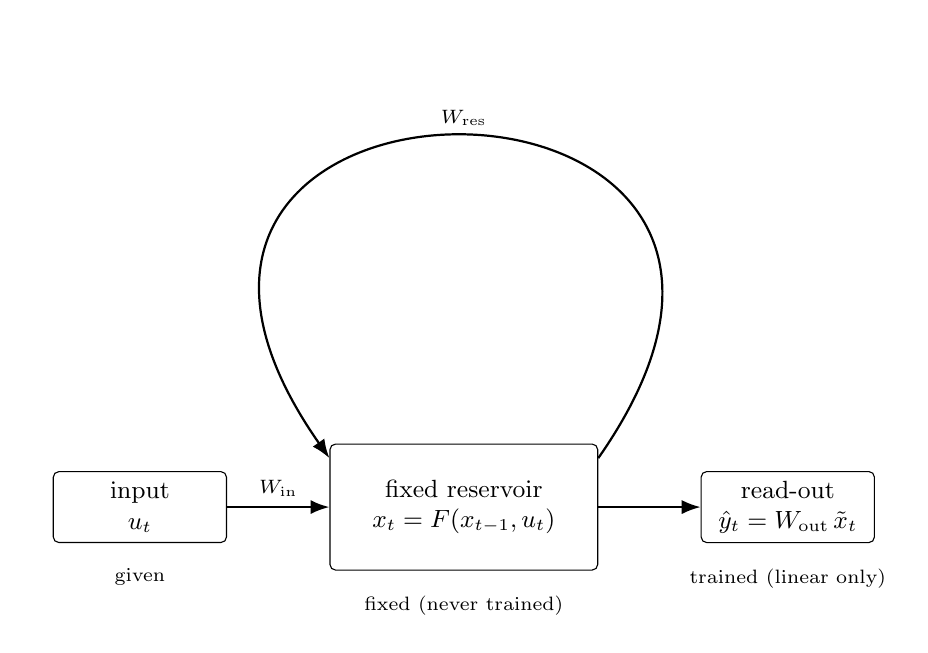
\begin{tikzpicture}[node distance=9mm and 13mm]
  \node[block] (in) {input\\$u_t$};
  \node[block, right=of in, minimum width=34mm, minimum height=16mm] (res)
    {fixed reservoir\\$x_t = F(x_{t-1}, u_t)$};
  \node[block, right=of res] (out) {read-out\\$\hat y_t = W_{\mathrm{out}}\,\tilde x_t$};
  \draw[arrow] (in) -- node[above,font=\scriptsize]{$W_{\mathrm{in}}$} (res);
  \draw[arrow] (res) -- (out);
  \draw[arrow] (res.20) to[out=55,in=125,looseness=5] node[above,font=\scriptsize]{$W_{\mathrm{res}}$} (res.160);
  \node[below=2mm of in, font=\scriptsize, align=center] {given};
  \node[below=2mm of res, font=\scriptsize, align=center] {fixed (never trained)};
  \node[below=2mm of out, font=\scriptsize, align=center] {trained (linear only)};
\end{tikzpicture}
\caption{The three-layer anatomy of reservoir computing. Only the read-out is
trained; the recurrent core is fixed at initialisation. In quantum reservoir
computing (Part~II) the middle block becomes an input-driven quantum channel
and the read-out acts on measured expectation values.}
\label{fig:rc-blocks}
\end{figure*}

\section{Echo state networks}
\label{sec:esn}

\subsection{State update and read-out}

The standard ESN maintains a state $x_t \in \R^{N_x}$ updated as
\begin{equation}
\begin{aligned}
  x_{t+1} \;=\;{}& (1-\alpha)\, x_t
  + \alpha\, f\!\left(W_{\mathrm{res}}\, x_t + W_{\mathrm{in}}\, u_{t+1} + b\right),\\
  & \alpha \in (0,1],
\end{aligned}
  \label{eq:leaky}
\end{equation}
whose leak rate $\alpha$ sets the intrinsic time scale of the reservoir and is
the single most important hyperparameter to match to the autocorrelation time
of the data (a point that returns, in quantum form, as the injection interval
$\Delta t$ in Parts~II and~VIII). The output is linear in the (possibly
augmented) state $\tilde x_t = (x_t^{\!\top}, 1)^{\!\top}$:
\begin{equation}
  \hat y_t \;=\; W_{\mathrm{out}}\, \tilde x_t .
  \label{eq:readout}
\end{equation}

Three conventions from Eq.~\eqref{eq:esn-update} onward hold throughout this
document. First, a \emph{washout}: the first $T_w$ states, which still remember
the arbitrary initial condition, are discarded before training. Second,
\emph{chronological splits}: training data strictly precede validation data,
which strictly precede test data; shuffled splits leak information through
autocorrelation and are one of the most common sources of inflated results in
time-series work. Third, all errors are reported as the normalised mean-square
error
\begin{equation}
  \NMSE \;=\; \frac{\sum_t \left(y_t - \hat y_t\right)^2}{\sum_t \left(y_t - \bar y\right)^2},
  \label{eq:nmse}
\end{equation}
for which the constant predictor $\hat y_t = \bar y$ scores exactly $1$.

\subsection{Ridge regression: derivation and practice}
\label{sec:ridge}

Collect the post-washout training states row-wise into
$X \in \R^{T\times (N_x+1)}$ and the targets into $y \in \R^{T}$. Ordinary
least squares minimises $\lVert Xw - y\rVert_2^2$, but reservoir states are
strongly collinear (neighbouring neurons see overlapping input histories), so
the normal-equations matrix $X^{\!\top}X$ is ill-conditioned and the unpenalised
solution overfits noise in the state trajectory. Ridge (Tikhonov) regression
minimises instead
\begin{equation}
  J(w) \;=\; \lVert Xw - y\rVert_2^2 + \lambda \lVert w\rVert_2^2,
  \qquad \lambda > 0 .
  \label{eq:ridge-objective}
\end{equation}
Setting $\nabla_w J = 2X^{\!\top}(Xw-y) + 2\lambda w = 0$ gives the closed form
\begin{equation}
  w^\star \;=\; \left(X^{\!\top}X + \lambda \id\right)^{-1} X^{\!\top} y .
  \label{eq:ridge-solution}
\end{equation}
Since $X^{\!\top}X \succeq 0$, the regularised matrix
$X^{\!\top}X + \lambda\id \succ 0$ is always invertible, and the objective
\eqref{eq:ridge-objective} is strictly convex, so $w^\star$ is the unique global
minimiser. In the singular-value decomposition $X = U\Sigma V^{\!\top}$ with
singular values $s_i$, Eq.~\eqref{eq:ridge-solution} becomes
\begin{equation}
  w^\star \;=\; \sum_i \frac{s_i}{s_i^2 + \lambda}\, \left(u_i^{\!\top} y\right) v_i ,
  \label{eq:ridge-svd}
\end{equation}
which exhibits ridge as a \emph{spectral filter}: directions of the state
space with $s_i^2 \gg \lambda$ pass through essentially untouched, while
directions with $s_i^2 \ll \lambda$ --- precisely the poorly excited, noise-dominated
ones --- are shrunk toward zero. This picture matters doubly in the quantum
setting, where each feature carries shot noise of known magnitude
(Part~IV): $\lambda$ is then not a nuisance parameter but the dial that trades
the reservoir's expressivity against its measurement noise. The penalty is
selected on held-out data --- either a chronological validation block or, when
that block is too short to be representative, by generalised cross-validation
on the training span; it is never tuned on the test set.

\begin{algorithm*}[t]
\caption{Echo state network training (batch, ridge read-out)}
\label{alg:esn}
\begin{algorithmic}[1]
\State draw $W_{\mathrm{in}}, W_{\mathrm{res}}, b$ at random; rescale $W_{\mathrm{res}}$ to spectral radius $\rho_{\mathrm{sr}}<1$
\State $x_0 \gets 0$
\For{$t = 1, \dots, T_{\mathrm{total}}$}
  \State $x_t \gets (1-\alpha)x_{t-1} + \alpha f(W_{\mathrm{res}}x_{t-1} + W_{\mathrm{in}}u_t + b)$
\EndFor
\State discard $t \le T_w$ (washout); stack remaining training states into $X$, targets into $y$
\State $W_{\mathrm{out}} \gets \left(X^{\!\top}X + \lambda\id\right)^{-1}X^{\!\top}y$ \Comment{$\lambda$ chosen on validation data}
\State \Return predictions $\hat y_t = W_{\mathrm{out}}\tilde x_t$ on the untouched test span
\end{algorithmic}
\end{algorithm*}

\section{What makes a good reservoir: the formal properties}
\label{sec:properties}

Three properties, introduced for ESNs but stated here in a form that transfers
verbatim to quantum reservoirs, separate systems that can compute from systems
that merely fluctuate.

\subsection{Echo state property}

\begin{definition}[Echo state property]
\label{def:esp}
A driven system with update $x_{t+1} = F(x_t, u_{t+1})$ on a compact state set
has the \emph{echo state property} (ESP) if for every input sequence
$\{u_t\}$ and every pair of initial conditions $x_0, x_0'$, the resulting
trajectories converge: $\lVert x_t - x_t'\rVert \to 0$ as $t \to \infty$.
Equivalently, after a transient the state is a function of the input history
alone, $x_t = \phi(\dots, u_{t-1}, u_t)$, independent of initialisation~\citep{jaeger2001echo}.
\end{definition}

The ESP is what makes the washout finite and the learned read-out
reproducible: without it, the ``features'' depend on an arbitrary initial
condition and the training problem is ill-posed. For the $\tanh$ ESN, a
sufficient condition is that the largest singular value of
$W_{\mathrm{res}}$ be below $1$; the everyday design rule of setting the
\emph{spectral radius} $\rho_{\mathrm{sr}}(W_{\mathrm{res}})$ slightly below
$1$ is a necessary condition (for zero input) and works well in practice,
though it is not sufficient in general~\citep{jaeger2001echo,lukosevicius2009reservoir}.
Extensions of the ESP to non-stationary systems and to subsystems --- needed when
only part of a larger system is observed, as is typical for quantum
reservoirs --- are developed in~\citet{kobayashi2024extending}.

\subsection{Fading memory}

\begin{definition}[Fading memory]
\label{def:fading}
A causal, time-invariant operator $M$ mapping input sequences to outputs has
\emph{fading memory} if inputs that agree on a recent window and differ only in
the remote past produce outputs that are close: for every $\varepsilon>0$
there exist $\delta>0$ and a decreasing weight sequence $w_k \downarrow 0$ such
that $\sup_k w_k\,|u_{t-k}-u'_{t-k}| < \delta$ implies
$|M[u]_t - M[u']_t| < \varepsilon$~\citep{boyd1985fading}.
\end{definition}

Fading memory formalises the intuition that a forecaster should care about the
recent past more than the distant past, with influence decaying continuously.
\citet{boyd1985fading} proved that operators with fading memory are exactly
those approximable by Volterra series --- the classical result that underlies all
reservoir universality theorems. In a reservoir with the ESP, fading memory is
automatic: the same contraction that erases the initial condition also erases
the remote input past. The tension at the heart of reservoir design is that
\emph{too much} contraction erases the recent past as well; the useful regime
lies near, but on the stable side of, the boundary
(Section~\ref{sec:edge-of-chaos}).

\subsection{Separation and the memory--nonlinearity trade-off}

The read-out is linear, so any two input histories that must be mapped to
different outputs must first be mapped, by the reservoir, to linearly
distinguishable states. This \emph{separation property}~\citep{maass2002realtime}
is the reservoir's expressivity requirement, complementary to the ESP's
stability requirement. A quantitative unification is the information-processing
capacity of \citet{dambre2012information}: for a reservoir with $N_x$
linearly independent state variables driven by i.i.d.\ input, the total
capacity to reconstruct \emph{any} orthonormal set of functions of the input
history (linear or nonlinear) is bounded by $N_x$, and saturates it for
fading-memory systems. Capacity spent on nonlinear functions is capacity not
available for linear memory --- the \emph{memory--nonlinearity trade-off} that
every reservoir, classical or quantum, must budget for the task at hand.

\subsection{Linear memory capacity}
\label{sec:memory-capacity}

The standard operational probe of memory is Jaeger's \emph{memory
capacity}~\citep{jaeger2001echo}. Drive the reservoir with i.i.d.\ scalar input
$u_t$, train a separate linear read-out to reconstruct each delayed input
$y_t = u_{t-d}$, and define
\begin{equation}
\begin{aligned}
  \mathrm{MC}_d \;&=\; \max_{w}\;
  \frac{\operatorname{cov}^2\!\left(u_{t-d},\, w^{\!\top}\tilde x_t\right)}
       {\operatorname{var}(u_{t-d})\,\operatorname{var}\!\left(w^{\!\top}\tilde x_t\right)},\\
  \mathrm{MC} \;&=\; \sum_{d=1}^{\infty} \mathrm{MC}_d .
\end{aligned}
  \label{eq:mc}
\end{equation}
Each $\mathrm{MC}_d \in [0,1]$ is the fraction of the delay-$d$ input variance
linearly recoverable from the state; $\mathrm{MC} \le N_x$ with equality
approached by linear reservoirs~\citep{jaeger2001echo,dambre2012information}.
In this document $\mathrm{MC}$ is estimated with delays up to $d_{\max}=25$ and
reported alongside every reservoir comparison (Part~VII), because a forecasting
model's usable history is bounded by it.

\subsection{Universality}
\label{sec:universality}

The formal justification for training only a linear read-out is a family of
universality theorems. For ESNs, \citet{grigoryeva2018echo} proved that echo
state networks with linear read-outs are universal: any causal, time-invariant
fading-memory filter on uniformly bounded inputs can be approximated to
arbitrary accuracy by an ESN of sufficient size. The proof route --- show the
family of reservoir functionals forms a polynomial algebra that separates
points, then apply Stone--Weierstrass --- is worth internalising because it
transfers: universality proofs for quantum reservoirs
(Part~II, Section~\ref{sec:qrc-universality}) follow the same architecture,
with the algebra generated by measured observables of the driven quantum
state~\citep{chen2019learning,nokkala2021gaussian,martinez2023finite}. Two
caveats temper the theorem's practical force. Universality is an existence
statement about \emph{some} sufficiently large reservoir, not a statement that
a random one of fixed size is good; and it says nothing about sample
efficiency. Both gaps are exactly where empirical reservoir quality --- and any
prospective quantum edge --- lives.

\section{Operating point: the edge of chaos}
\label{sec:edge-of-chaos}

For a fixed task, reservoir performance as a function of the dynamical regime
is strikingly non-monotonic. Deep in the ordered (strongly contracting) regime
the state barely responds to input and memory is short; deep in the chaotic
regime the ESP fails and the state amplifies microscopic differences until the
input signal is scrambled. Performance typically peaks near the
order--chaos boundary --- the \emph{edge of chaos} --- where correlations are long
but reproducibility survives~\citep{boedecker2012information}. For ESNs the
practical dials are the spectral radius $\rho_{\mathrm{sr}}$, the input
scaling, and the leak rate $\alpha$; systematic constraints on their joint
choice are mapped in~\citet{storm2022constraints}. Two further classical
lessons recur in the quantum setting. First, reservoirs whose dynamics have a
symmetry the task must break (for the $\tanh$ ESN, the odd symmetry
$f(-z)=-f(z)$) fail on symmetric tasks unless the symmetry is explicitly
broken, e.g.\ by biases~\citep{herteux2020breaking}; the quantum analogue ---
symmetries of the reservoir Hamiltonian polluting chaos diagnostics and
constraining which observables carry information --- appears in Part~VIII.
Second, the edge is a property of the \emph{driven} system, not the autonomous
one: input strength shifts it, so the operating point must be tuned with the
data in the loop. In quantum many-body reservoirs the edge acquires a second,
temporal dimension (the injection interval relative to the Thouless time),
identified by \citet{kobayashi2026edge} and reproduced numerically in Part~VII
of this document.

\section{Reservoir computing for chaotic and geophysical systems}
\label{sec:rc-chaos}

The application benchmark that made modern RC famous is model-free prediction
of chaos. \citet{jaeger2004harnessing} demonstrated orders-of-magnitude
improvements in Mackey--Glass~\citep{mackey1977oscillation} prediction;
\citet{pathak2018model} showed that a parallelised ESN can forecast the
Kuramoto--Sivashinsky equation for multiple Lyapunov times and reproduce its
climate (attractor statistics); hybrids of reservoirs with imperfect
knowledge-based models outperform either alone~\citep{pathak2018hybrid};
and \citet{arcomano2020machine} scaled the approach to a global atmospheric
model, establishing RC as a serious tool for the weather--climate problem class
this document targets. Careful comparisons find well-tuned reservoirs
competitive with, and far cheaper to train than, backpropagated recurrent
networks on these tasks~\citep{vlachas2020backpropagation}. Chaotic benchmarks
(Lorenz-63~\citep{lorenz1963deterministic}, Mackey--Glass) therefore serve in
this document as controlled stand-ins for the harder, noisier renewable and
climate series of Part~VI, and the NARMA family serves as the standard
memory-plus-nonlinearity stress test.

\section{Baseline discipline}
\label{sec:baselines}

Because Parts~VI--VIII evaluate quantum reservoirs against economically
meaningful forecasting tasks, the classical baselines are fixed here once and
used everywhere. (i)~\emph{Mean predictor}: $\NMSE = 1$ by construction; drawn
as a horizontal line on every error axis. (ii)~\emph{Persistence}:
$\hat y_{t+h} = y_t$; embarrassingly strong on slowly varying series such as
solar irradiance at short horizons, and the baseline most often missing from
overclaiming studies. (iii)~\emph{Linear auto-regression on $p$ lags}: the
cheapest model with memory; any nonlinear reservoir must beat it to justify
its existence. (iv)~\emph{Size-matched ESN}: Eqs.~\eqref{eq:leaky} and
\eqref{eq:ridge-solution} with the number of read-out features equal to the
quantum feature count, so comparisons are at matched read-out capacity.
A quantum reservoir result in this document is reported as interesting only
relative to all four, and Part~VIII adds a fifth, quantum-internal control:
a structureless (Haar-random) quantum reservoir of the same size.

\parttitle{II}{Quantum Foundations and the Quantum Reservoir Computing Formulation}

\section{States, observables, and measurement}
\label{sec:quantum-states}

This part fixes the quantum-mechanical machinery in exactly the depth the rest
of the document uses; standard references are
\citet{nielsen2010quantum} for closed-system and circuit material and
\citet{breuer2002theory} for open systems.

A system of $n$ qubits lives on the Hilbert space
$\Hil = (\C^2)^{\otimes n}$ of dimension $d = 2^n$. Pure states are unit
vectors $\ket{\psi} \in \Hil$; the general state is a \emph{density matrix}
$\rho$, a positive semidefinite operator with $\tr\rho = 1$, encompassing pure
states ($\rho = \ketbra{\psi}{\psi}$, $\tr\rho^2 = 1$) and statistical
mixtures ($\tr\rho^2 < 1$). Two structural facts about $\rho$ drive everything
in this document. First, the \emph{exponential dimension}: $\rho$ has
$d^2 - 1 = 4^n - 1$ real parameters, so an $n$-qubit reservoir carries a state
space whose dimension no polynomial-size classical reservoir matches
parameter-for-parameter. Second, the \emph{partial trace}: for a bipartite
system $AB$, the state of $B$ alone is $\rho_B = \tr_A \rho_{AB}$, the unique
operator reproducing all local measurement statistics on $B$. The partial
trace is the mechanism by which the Fujii--Nakajima reservoir
(Section~\ref{sec:qrc-update}) forgets its input qubit while retaining
correlations in the rest --- memory by entanglement.

Observables are Hermitian operators $O$; the Born rule gives the expectation
value $\ev{O} = \tr(O\rho)$. The $n$-qubit Pauli operators
$\{ \id, X, Y, Z \}^{\otimes n}$ form an orthogonal operator basis, so the set
of expectation values of all Pauli strings determines $\rho$ completely; a
reservoir read-out measures a small, fixed subset of them --- in this document
the single-qubit $\ev{Z_i}$, $\ev{X_i}$ and two-qubit $\ev{Z_i Z_j}$. The most
general measurement is a positive operator-valued measure (POVM): a set
$\{E_m\}$ with $E_m \succeq 0$ and $\sum_m E_m = \id$, outcome $m$ occurring
with probability $p_m = \tr(E_m \rho)$. Projective measurement of a qubit in
the computational basis is the special case $E_0 = \ketbra{0}{0}$,
$E_1 = \ketbra{1}{1}$, and is the only primitive current digital hardware
exposes; every ``expectation value'' in an experiment is a finite-sample
average of projective outcomes, a fact whose statistical consequences
(Section~\ref{sec:shot-noise}) shape reservoir design as strongly as any
Hamiltonian choice.

\section{Dynamics: unitaries, channels, and the Lindblad equation}
\label{sec:channels}

\subsection{Closed systems}

A closed system evolves unitarily, $\rho \mapsto U \rho U^\dagger$ with
$U = e^{-iHt}$ generated by a Hamiltonian $H$ (units with $\hbar = 1$
throughout). Unitary evolution is an isometry of state space: it can never
contract two distinct initial states toward each other. An immediate and
frequently overlooked consequence for reservoir computing is that
\emph{a strictly closed quantum system cannot have the echo state property}:
initial-condition differences persist forever, so fading memory
(Definition~\ref{def:fading}) fails. Every working quantum reservoir therefore
contains an explicitly non-unitary element --- an input-injection step that
discards a subsystem, engineered dissipation, or measurement --- and identifying
where that contraction enters is the first question to ask of any proposed
architecture~\citep{chen2019learning,sannia2024dissipation,kobayashi2024coherence}.

\subsection{Quantum channels}

The general physical evolution of a possibly open system is a
\emph{quantum channel}: a completely positive, trace-preserving (CPTP) linear
map $\map{E}$ on density matrices. Every channel admits a Kraus representation
\begin{equation}
  \map{E}(\rho) \;=\; \sum_j K_j \rho K_j^\dagger,
  \qquad
  \sum_j K_j^\dagger K_j = \id ,
  \label{eq:kraus}
\end{equation}
and, equivalently (Stinespring), can be realised as a unitary on the system
plus an environment followed by a partial trace over the environment.
Complete positivity (positivity of $\map{E}\otimes\id$ on any enlarged system)
is what guarantees the map remains physical when the system is entangled with
a bystander; trace preservation is probability conservation. Channels are
exactly the update maps a quantum reservoir may use, and their key analytic
property for this document is \emph{contractivity}: every channel is
non-expansive in trace distance,
$\tfrac12\lVert\map{E}(\rho)-\map{E}(\sigma)\rVert_1 \le
 \tfrac12\lVert\rho-\sigma\rVert_1$,
with strict contraction (for generic state pairs) precisely when the channel
has a non-unitary part. Strict contractivity is the quantum form of the echo
state property (Section~\ref{sec:quantum-esp}).

A convenient linear-algebraic handle used repeatedly in Parts~VII--VIII is the
\emph{Pauli transfer matrix} (PTM): expanding
$\rho = \tfrac1d\sum_\alpha r_\alpha P_\alpha$ over Pauli strings $P_\alpha$
turns a channel into a real matrix $T$ acting on the coefficient vector $r$,
with the unital block's spectral radius governing how fast initial-condition
information decays. \citet{kobayashi2024coherence} sharpen this picture for
reservoirs: fading memory requires the input-independent part of the PTM to be
strictly contractive on the traceless sector, while useful input sensitivity
requires a \emph{coherence influx} --- an input-dependent affine part that keeps
re-exciting the contracting state. Channels that contract without influx (for
example, uniform depolarisation toward the maximally mixed state) satisfy the
ESP but forget the input as fast as the initial condition, and score near
$\NMSE=1$; the distinction is demonstrated numerically in
Part~IV's noise studies.

\subsection{Continuous-time open dynamics}

When the environment coupling is weak and memoryless (Born--Markov), the state
obeys the Gorini--Kossakowski--Sudarshan--Lindblad master
equation~\citep{lindblad1976generators,gorini1976completely}
\begin{equation}
\begin{aligned}
  \dot\rho \;=\; \map{L}(\rho)
  \;&=\; -i[H,\rho]\\
  &\;+\; \sum_k \gamma_k \left( L_k \rho L_k^\dagger
        - \tfrac12\{L_k^\dagger L_k, \rho\} \right),
\end{aligned}
  \label{eq:lindblad}
\end{equation}
whose solution $\rho(t) = e^{\map{L}t}\rho(0)$ is a CPTP semigroup. The jump
operators $L_k$ model the dissipation channels of real hardware: amplitude
damping ($L = \sigma^- = \ketbra{0}{1}$, rate $1/T_1$) relaxes excitation
toward $\ket{0}$; pure dephasing ($L = Z$, rate contribution to $1/T_2$)
destroys phase coherence without moving populations. The distinction is not
cosmetic for reservoirs. Amplitude damping drives the system toward a
\emph{polarised} fixed point ($\ket{0}^{\otimes n}$) from which fresh input
rotations produce large, input-dependent signals, so moderate $T_1$ decay can
supply exactly the contraction the ESP needs while preserving
responsiveness~\citep{sannia2024dissipation,domingo2022optimal}. Strong
dephasing, by contrast, drives states toward the diagonal and, combined with
depolarising elements, toward the maximally mixed state, where all bounded
observables concentrate and the signal is erased --- contraction without
coherence influx~\citep{kobayashi2024coherence,xiong2025role}. ``Noise'' is
therefore neither friend nor enemy of QRC in general; \emph{which} noise, at
what rate, relative to the injection interval, is a design axis
(Part~VIII).

\section{The quantum reservoir computing formulation}
\label{sec:qrc-formulation}

\subsection{State update and read-out}
\label{sec:qrc-update}

A quantum reservoir computer replaces the classical update
Eq.~\eqref{eq:esn-update} by an input-dependent channel acting on the
reservoir's density matrix,
\begin{equation}
\begin{aligned}
  \rho_{t+1}
  \;=\;{}&
  U_{\Delta t}\,
  \Bigl( \ketbra{\psi_{u_{t+1}}}{\psi_{u_{t+1}}} \,\otimes\, \tr_1 \rho_t \Bigr)\,
  U_{\Delta t}^\dagger,\\
  & \ket{\psi_u} = \sqrt{1-u}\,\ket{0} + \sqrt{u}\,\ket{1},
\end{aligned}
  \label{eq:fn-update}
\end{equation}
with $U_{\Delta t} = e^{-iH\Delta t}$ and
\begin{equation}
\begin{aligned}
  H \;=\;{}& \sum_{i<j} J_{ij}\, X_i X_j \;+\; \tfrac{h}{2} \sum_i Z_i ,\\
  & J_{ij} \sim \mathcal{U}[-J/2, J/2].
\end{aligned}
  \label{eq:fn-hamiltonian}
\end{equation}
Equation~\eqref{eq:fn-update} is a legitimate CPTP map (a partial trace, a
tensor product with a fresh state, and a unitary), and each ingredient plays a
distinct role: the partial trace $\tr_1$ is the contraction that grants the
ESP and fading memory; the re-preparation $\ketbra{\psi_u}{\psi_u}$ is the
coherence influx that keeps the reservoir responsive; and the entangling
unitary $U_{\Delta t}$ spreads the fresh input into the retained qubits, where
it interferes with the stored history. Figure~\ref{fig:qrc-pipeline} shows the
full pipeline including measurement and the classical read-out.

\begin{figure*}[t]
\centering
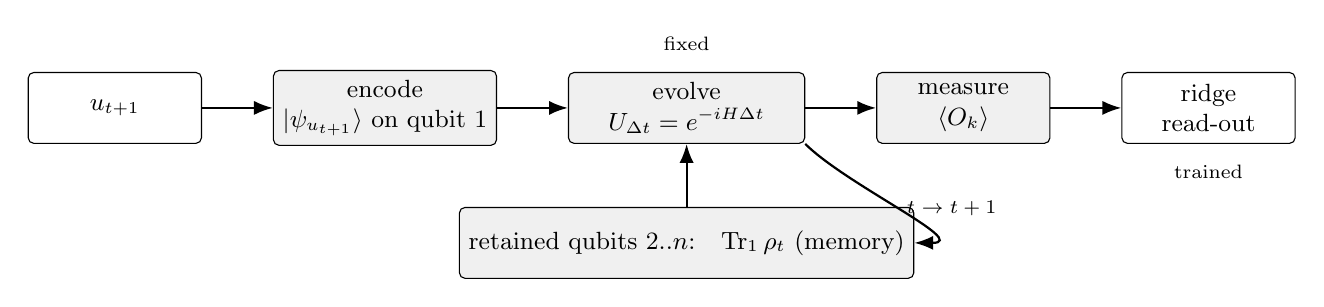
\begin{tikzpicture}[node distance=7mm and 9mm]
  \node[block] (u) {$u_{t+1}$};
  \node[qblock, right=of u] (enc) {encode\\$\ket{\psi_{u_{t+1}}}$ on qubit 1};
  \node[qblock, right=of enc, minimum width=30mm] (evo) {evolve\\$U_{\Delta t}=e^{-iH\Delta t}$};
  \node[qblock, right=of evo] (meas) {measure\\$\ev{O_k}$};
  \node[block, right=of meas] (ro) {ridge\\read-out};
  \node[below=8mm of evo, qblock, minimum width=30mm] (mem) {retained qubits $2..n$:\quad $\tr_1\rho_t$ (memory)};
  \draw[arrow] (u) -- (enc);
  \draw[arrow] (enc) -- (evo);
  \draw[arrow] (evo) -- (meas);
  \draw[arrow] (meas) -- (ro);
  \draw[arrow] (mem.north) -- (evo.south);
  \draw[arrow] (evo.south east) to[out=-45,in=0] node[right,font=\scriptsize]{$t\to t+1$} (mem.east);
  \node[below=1.5mm of ro, font=\scriptsize] {trained};
  \node[above=1.5mm of evo, font=\scriptsize] {fixed};
\end{tikzpicture}
\caption{One step of the Fujii--Nakajima quantum reservoir,
Eq.~\eqref{eq:fn-update}. The input qubit is re-prepared each step (coherence
influx); the remaining qubits carry the fading memory forward; measurement of
a fixed observable set feeds the only trained component, a linear read-out.}
\label{fig:qrc-pipeline}
\end{figure*}

\subsection{Where the nonlinearity enters}
\label{sec:nonlinearity}

Equation~\eqref{eq:qrc-update} is \emph{linear in $\rho$}, and
Eq.~\eqref{eq:qrc-features} is linear too, so a natural worry is that the
whole machine is linear and the read-out learns nothing an autoregression
could not. The worry dissolves once one asks: nonlinear \emph{in what}? Three
distinct mechanisms make the features nonlinear in the \emph{input history},
which is the variable that matters.

\emph{(i) Nonlinear encoding.} The map $u \mapsto \ketbra{\psi_u}{\psi_u}$ in
Eq.~\eqref{eq:fn-update} is quadratic in the amplitudes
$(\sqrt{1-u},\sqrt{u})$, and rotation encodings $R_Y(\gamma u)$ used in
Parts~III--IV make expectation values trigonometric polynomials in $u$. For
parameterised re-uploading circuits this is a theorem: the output is a
truncated Fourier series in the encoded variables, with the accessible
frequency spectrum set by the encoding generators and their
repetitions~\citep{schuld2021effect}. The encoding scale $\gamma$ therefore
controls how much of the read-out's approximation power sits in high
harmonics --- the practical saturation effect quantified in Part~IV.

\emph{(ii) Products through the update composition.} Because the input enters
the channel multiplicatively (the new state is a \emph{product}
$\ketbra{\psi_u}{\psi_u} \otimes \tr_1\rho_t$, then conjugated), composing $T$
steps produces expectation values containing products of functions of
$u_t, u_{t-1}, \dots$ --- exactly the cross terms a NARMA-type target needs.
In the PTM picture: the affine input drive is state-dependent through the
tensor-product structure, so the composed map is polynomial, not affine, in
the input sequence.

\emph{(iii) Measurement-derived nonlinearity.} Any protocol that feeds
measured outcomes back into the drive (Part~III's measurement-based and
feedback architectures~\citep{kobayashi2024feedback,franceschetto2024harnessing}),
or that computes nonlinear functions of estimated expectations classically
(e.g.\ including products $\ev{Z_i}\ev{Z_j}$ as features), imports an
additional, explicitly nonlinear stage. The second-moment observables
$\ev{Z_iZ_j}$ used throughout this document are linear in $\rho$ but carry
information about correlations that no set of single-qubit means determines,
which is why adding them raised the effective feature rank so sharply in the
Part~IV experiments.

What the linearity of Eq.~\eqref{eq:qrc-update} \emph{does} imply is an exact
finite-dimensional bookkeeping: the reservoir state is a vector in
$\R^{4^n-1}$ evolving affinely for each fixed input value, so QRC never
escapes the information-processing capacity bound of
\citet{dambre2012information} --- at most $4^n-1$ independent functionals, and
in practice as many as the \emph{measured, well-conditioned} directions
support. The realistic promise of QRC is therefore not unbounded expressivity
but a large, physically generated feature bank per physical
component~\citep{fujii2017harnessing,mujal2021opportunities}, whose usable
fraction is decided by measurement statistics
(Section~\ref{sec:shot-noise}).

\subsection{Quantum echo state property and fading memory}
\label{sec:quantum-esp}

\begin{definition}[Quantum ESP]
\label{def:qesp}
The reservoir family $\{\map{E}_{\theta,u}\}$ has the echo state property if
for every admissible input sequence and every pair of initial states
$\rho_0, \rho_0'$,
$\lVert \rho_t - \rho_t' \rVert_1 \to 0$ as $t\to\infty$, where
$\rho_t = \map{E}_{\theta,u_t}\circ\cdots\circ\map{E}_{\theta,u_1}(\rho_0)$.
\end{definition}

Sufficient conditions mirror the classical ones with contraction coefficients
replacing spectral radii: if every $\map{E}_{\theta,u}$ is a strict
contraction in trace distance with a uniform coefficient $c<1$, initial-state
information decays as $c^{\,t}$ and the ESP holds together with fading
memory~\citep{chen2019learning,chen2020temporal,martinez2023finite}. For the
Fujii--Nakajima update the contraction is supplied structurally by the partial
trace; for dissipative reservoirs, by the Lindbladian's spectral gap; for
measurement-based schemes, by the state collapse itself. The refinements a
practitioner needs are (a) the \emph{nonstationary/subspace ESP} of
\citet{kobayashi2024extending}, which handles reservoirs where only a
subsystem or a conditioned sector must forget, and (b) the coherence-influx
criterion of \citet{kobayashi2024coherence} separating useful contraction
(toward an input-sensitive, polarised region) from destructive contraction
(toward the maximally mixed state). Both are cheap to check numerically from
the PTM and are part of the validation suite shipped with this document's code.

\subsection{Universality}
\label{sec:qrc-universality}

Universality theorems for QRC parallel Section~\ref{sec:universality}.
\citet{chen2019learning} established that families of dissipative quantum
systems with contractive dynamics and polynomial read-outs realise dense
subsets of fading-memory maps; \citet{chen2020temporal} adapted the
construction to gate-model devices with a hardware demonstration;
\citet{nokkala2021gaussian} proved universality for continuous-variable
Gaussian reservoirs, notable because Gaussian dynamics are efficiently
classically simulable --- universality alone therefore confers no quantum
advantage; and \citet{martinez2023finite} gave a finite-dimensional treatment
identifying which ingredients (contraction, input-dependence, read-out
algebra) are load-bearing. The practical reading is the same as in the
classical case: universality licenses the paradigm, and everything
interesting --- sample efficiency, feature quality per shot, robustness ---
is decided by the concrete architecture, which is Part~III's subject.

\section{Extracting features: multiplexing and measurement back-action}
\label{sec:extraction}

\subsection{Temporal and spatial multiplexing}

The measured feature count $K$, not the Hilbert-space dimension, bounds the
read-out. Two standard tricks enlarge $K$ at fixed hardware.
\emph{Temporal multiplexing}~\citep{fujii2017harnessing} samples the
observables at $V$ intermediate times within each injection interval,
$x_t^{(k,v)} = \tr\bigl(O_k\, e^{-iH v\Delta t/V}\rho_t^{\mathrm{inj}}
e^{+iH v\Delta t/V}\bigr)$, multiplying the feature count by $V$ (the
\emph{virtual nodes}); the document's reference implementation uses $V=4$.
\emph{Spatial multiplexing}~\citep{nakajima2019boosting} runs $M$ independent
small reservoirs on disjoint qubit sets and concatenates their features,
trading entanglement breadth for shot-parallelism and noise isolation ---
usually the right trade on current hardware, and the reason Part~VII's
pipelines shard across small registers rather than maximising register size.

\subsection{Measurement back-action: the four protocols}
\label{sec:backaction}

Equation~\eqref{eq:qrc-features} silently assumes access to exact expectation
values of an undisturbed state, but projective measurement collapses the state
it reads. Four protocols manage the conflict, and choosing among them is a
first-class architectural decision~\citep{mujal2023time}:

\emph{Restart (rewind).} To obtain features at step $t$, re-run the input
sequence from scratch (in practice, from a finite window of length $L$, valid
precisely because fading memory suppresses older inputs) and measure once at
the end. Cost per time step grows with $L\times$ shots, but the state before
measurement is exact. All gate-model examples in Part~IV use this protocol.

\emph{Ensemble.} Run many copies in parallel and measure each copy once per
step --- natural for NMR spin ensembles~\citep{negoro2018machine} and atomic
ensembles, where the ``copies'' are physical molecules or atoms.

\emph{Weak measurement.} Couple a meter weakly, extracting a little
information per step at the cost of a little disturbance;
\citet{mujal2023time} quantify the regime where the running estimate is
accurate while the reservoir dynamics remain effectively intact, and
\citet{franceschetto2024harnessing} show the disturbance itself can be
harnessed as a computational resource.

\emph{Mid-circuit measurement and reset.} Measure a designated subset of
qubits projectively each step and reset it for the next injection --- the
hardware-native realisation of Eq.~\eqref{eq:fn-update}'s partial trace. Its
decisive property, established theoretically and on superconducting hardware
by \citet{hu2024overcoming} (the NISQRC scheme), is that the usable memory
time is set by the \emph{engineered} contraction, not by $T_1/T_2$: the
persistent qubits are refreshed through interaction rather than left to
decohere, so temporal processing can run for durations far exceeding
coherence times. Part~IV demonstrates the primitive in Qiskit with per-step
classical registers.

\subsection{Shot noise}
\label{sec:shot-noise}

With $S$ projective shots, the estimator of a Pauli expectation
$z = \ev{P}$ is a scaled binomial average with standard deviation
\begin{equation}
  \sigma(\hat z) \;=\; \sqrt{\frac{1-z^2}{S}} \;\le\; \frac{1}{\sqrt{S}},
  \label{eq:shot-noise}
\end{equation}
so halving the feature noise costs $4\times$ the shots. Shot noise enters the
ridge problem as noise on the \emph{design matrix}, not the targets, which
biases as well as inflates variance; its interaction with the regulariser is
derived and measured in Part~IV, and its fundamental consequences ---
an effective, noise-dependent cap on the number of usable feature directions
(\emph{eigentasks}) --- are established in
\citet{hu2023tackling} and, for training specifically, in
\citet{ahmed2025optimal}. Two design rules follow and are enforced throughout
this document: always measure the exact-simulation ceiling before any shot
study, so that shot effects are not confused with architectural ones; and
treat $S$ as a first-class resource reported next to every hardware-relevant
number, since a reservoir that needs $10^6$ shots per feature to beat a
\num{30}-neuron ESN has lost on the only axis that counts.

\subsection{Exponential concentration}
\label{sec:concentration}

The scaling threat specific to quantum feature maps is
\emph{concentration}: for deep scrambling dynamics, random circuits, or
noise-dominated evolution, local observables concentrate exponentially in $n$
around state-independent values, so the input-dependent signal shrinks beneath
any fixed shot budget --- the reservoir analogue of barren
plateaus~\citep{mcclean2018barren}. For QRC the phenomenon and its
symmetry-resolved structure are analysed in
\citet{sannia2025exponential,xiong2025role}: scrambling that is useful at
small depth becomes signal-destroying at large depth or size, and noise
accelerates the collapse. The operational defences --- moderate evolution per
step, polarised fixed points, local observables on shallow light-cones,
spatial multiplexing instead of monolithic growth, and empirical monitoring of
feature variance and effective rank as $n$ grows --- recur as design principles
in Part~VIII. Concentration is the single strongest reason this document's
claims are confined to the small-$n$ regime actually simulated, and why no
extrapolation to large registers is offered anywhere.

\parttitle{III}{Architectures for Quantum Reservoirs}

\noindent
This part surveys the principal quantum reservoir architectures. Each entry
follows one template --- \emph{model and update; encoding; observables;
strengths; weaknesses; hardware suitability; extensions} --- so that the
comparison table (Table~\ref{tab:arch-compare}) can be read as a summary
rather than a substitute. Throughout, ``update'' refers to the concrete form
taken by the channel $\map{E}_{\theta,u}$ of Eq.~\eqref{eq:qrc-update}, and
epistemic labels follow the frontmatter conventions: entries note explicitly
whether the architecture has been demonstrated on hardware or only in
simulation.

\section{Ising / disordered-Hamiltonian reservoirs}
\label{sec:arch-ising}

\emph{Model and update.} The original and still most-studied QRC: $n$ qubits
under a fixed disordered Hamiltonian, canonically the transverse-field Ising
form of Eq.~\eqref{eq:fn-hamiltonian}, driven by the injection map
Eq.~\eqref{eq:fn-update}~\citep{fujii2017harnessing}. One time step is: replace
the input qubit's state, evolve unitarily for $\Delta t$, read observables
(optionally at $V$ intermediate times).

\emph{Encoding.} State replacement
$\ket{\psi_u}=\sqrt{1-u}\ket0+\sqrt{u}\ket1$ (amplitude encoding of a scalar);
multivariate inputs use several input qubits or a rotation encoding
$R_Y(\gamma u^{(j)})$ per component.

\emph{Observables.} $\ev{Z_i}$ per virtual node; $\ev{Z_iZ_j}$ at the final
virtual node; $\ev{X_i}$ where transverse coherences are informative.

\emph{Strengths.} Conceptually clean separation of memory (retained qubits)
and influx (re-prepared qubit); strong small-system benchmark record ---
$5$--$7$ qubits emulating ESNs of hundreds of nodes on NARMA and
Mackey--Glass in exact simulation~\citep{fujii2017harnessing,kutvonen2020optimizing};
dynamical regime controllable through $(J\Delta t, h/J$, disorder$)$ with the
performance-optimal region tied to the ergodic--localised boundary
\citep{martinez2021dynamical} and, in time, to the edge of many-body chaos
\citep{kobayashi2026edge}.

\emph{Weaknesses.} Exact density-matrix simulation is $O(4^n)$, capping
honest classical study near $n\!\approx\!12$--$14$; on gate hardware the
continuous evolution must be Trotterised and the injection realised by
mid-circuit reset, importing circuit noise; scalar drive on a single input
qubit yields features with low effective rank unless multiplexing and
two-body observables are used (measured in Part~IV).

\emph{Hardware suitability.} Natural on platforms with always-on couplings
(NMR ensembles, where it was demonstrated experimentally
\citep{negoro2018machine}; spin lattices); digital superconducting/trapped-ion
realisations via Trotterisation plus mid-circuit reset
\citep{chen2020temporal,hu2024overcoming,yasuda2023quantum}.

\emph{Extensions.} Higher-order reservoirs coupling multiple registers
\citep{tran2020higher}; artificial memory restriction to tune the
memory--nonlinearity balance \citep{cindrak2024enhancing}; engineered
dissipation replacing the partial trace \citep{sannia2024dissipation}.

\section{Spin-chain reservoirs with local structure}
\label{sec:arch-chain}

\emph{Model and update.} As Section~\ref{sec:arch-ising} but with
nearest-neighbour chains or lattices,
$H=\sum_i J_i\,\sigma_i\sigma_{i+1} + \sum_i h_i Z_i$ (Ising, XX, XXZ, or
Heisenberg variants), matching hardware connectivity. On-site disorder
$h_i \sim \mathcal{U}[-W,W]$ provides a clean chaos dial: sweeping $W$ moves
the level-spacing statistics between Wigner--Dyson ($\ev{r}\!\approx\!0.53$,
ergodic) and Poisson ($\ev{r}\!\approx\!0.39$, localised), with reservoir
performance peaking near the crossover
\citep{martinez2021dynamical,kobayashi2026edge}.

\emph{Encoding/Observables.} As above; local observables are natural because
information spreads along the chain at a finite (Lieb--Robinson) velocity,
which also localises the causal cone --- useful for shallow hardware
implementations.

\emph{Strengths.} Direct map to linear-coupling hardware (superconducting
chains, ion chains, Rydberg arrays); physically meaningful dynamical-phase
dial; disorder-free operating points also exist (clean lattices work in
suitable regimes~\citep{llodra2025atomic}), which matters for analog platforms
where per-site disorder is hard to program.

\emph{Weaknesses.} Finite information velocity means distant qubits take
several steps to feel the input --- memory arrives with latency; symmetries of
clean chains (e.g.\ total-$Z$ conservation in XXZ at zero field) restrict
which observables respond and pollute chaos diagnostics unless resolved by
symmetry sector (Part~VIII).

\emph{Hardware suitability.} The best match to fixed-topology digital devices;
the reference geometry for Part~IV's transpilation study.

\emph{Extensions.} Two-dimensional lattices; quasiperiodic fields;
programmable-geometry analog arrays (Section~\ref{sec:arch-rydberg}).

\section{Random-circuit reservoirs (restart protocol)}
\label{sec:arch-circuit}

\emph{Model and update.} A fixed, randomly drawn shallow circuit block $W$
(random single-qubit rotations plus an entangling brickwork) interleaved with
input-encoding rotations; the reservoir ``state'' is implicit in the restart
protocol of Section~\ref{sec:backaction}: for each $t$, a fresh circuit
re-uploads the last $L$ inputs,
$\ket{\phi_t} = \prod_{j=1}^{L} \bigl[\,W\, R(u_{t-L+j})\,\bigr]\ket{0}^{\otimes n}$,
and is measured once~\citep{chen2020temporal}. The recurrence-free variant of
\citet{ahmed2024prediction} formalises the window as an explicit delay
embedding and shows it inherits reservoir guarantees while eliminating
back-action bookkeeping entirely.

\emph{Encoding.} Angle re-uploading $R_Y(\gamma g_i u)$ with fixed random
gains $g_i$; the output is a truncated Fourier series in the inputs with
spectrum set by $\gamma$ and the number of repetitions
\citep{schuld2021effect}.

\emph{Observables.} $\ev{Z_i}$, $\ev{X_i}$, $\ev{Z_iZ_j}$ from terminal
measurement; all obtainable from two measurement bases.

\emph{Strengths.} Trivially portable across gate hardware --- no mid-circuit
operations required; state before measurement is exact, so shot noise is the
only estimator error; window length $L$ is an honest, explicit memory budget;
the architecture used by most current hardware demonstrations, including the
energy-forecasting studies of Part~VI~\citep{chen2020temporal,odo2026quantum}.

\emph{Weaknesses.} Cost per time step scales with $L$ (the window is
re-executed each step); memory is hard-truncated at $L$ rather than fading;
as a pure feature map it can underperform genuinely recurrent reservoirs on
long-memory tasks --- quantified in Part~IV, where the windowed PennyLane model
trails the recurrent simulation on ENSO by a wide margin; deep random blocks
concentrate (Section~\ref{sec:concentration}), so depth must stay moderate.

\emph{Hardware suitability.} Any gate-model device; the default choice for
first hardware experiments.

\emph{Extensions.} Encoding-scale tuning by gradient descent (Part~IV);
classical-lag augmentation into the read-out; noise-as-nonlinearity variants
(Section~\ref{sec:arch-dissipative}).

\section{Measurement-based and feedback reservoirs}
\label{sec:arch-measurement}

\emph{Model and update.} Measurement is promoted from read-out to dynamical
ingredient. In mid-circuit-reset (NISQRC) form, a designated I/O subset is
measured and reset every step while persistent qubits carry memory
\citep{hu2024overcoming}; in weak-measurement form, a continuous meter record
is the feature stream \citep{mujal2023time,franceschetto2024harnessing}; in
feedback form, measured outcomes condition subsequent gates or drives,
$\map{E}_{u,m_t}$ with $m_t$ the outcome, injecting explicit nonlinearity and
enabling closed-loop tasks \citep{kobayashi2024feedback}.

\emph{Encoding/Observables.} As the host architecture; the distinctive output
is the \emph{record} $\{m_t\}$ or per-step estimated expectations.

\emph{Strengths.} Memory decoupled from $T_1/T_2$ (the NISQRC result ---
hardware-demonstrated on IBM devices \citep{hu2024overcoming,yasuda2023quantum});
online operation on a single copy rather than restart; feedback adds
nonlinearity a linear channel cannot express.

\emph{Weaknesses.} Conditional logic and fast reset are demanding hardware
primitives with their own error budgets; the conditioned dynamics are harder
to analyse (the relevant ESP is the subspace/nonstationary form of
\citet{kobayashi2024extending}); weak-measurement gain must be tuned against
disturbance.

\emph{Hardware suitability.} Superconducting platforms with dynamic circuits
(demonstrated); trapped ions with mid-circuit detection; photonics with
homodyne records (Section~\ref{sec:arch-cv}).

\emph{Extensions.} Back-action-as-resource protocols
\citep{franceschetto2024harnessing}; reservoir-assisted quantum-state
measurement, inverting the roles of system and meter
\citep{angelatos2021reservoir}.

\section{Dissipative and noise-driven reservoirs}
\label{sec:arch-dissipative}

\emph{Model and update.} The contraction required by
Definition~\ref{def:qesp} is supplied by engineered or intrinsic open-system
dynamics: evolve under Eq.~\eqref{eq:lindblad} between injections, or, on
gate hardware, let the device's own noise channels act
\citep{chen2019learning,sannia2024dissipation}. In the ``natural quantum
reservoir'' of \citet{suzuki2022natural}, an IBM processor's intrinsic
dissipation supplied both the fading memory and useful nonlinearity, with the
demonstration run on hardware.

\emph{Encoding.} Any of the preceding; dissipation is a property of the
between-injection dynamics, not the encoding.

\emph{Observables.} As host architecture.

\emph{Strengths.} Turns the platform's unavoidable imperfection into the
stability mechanism; fixed-point structure is designable --- amplitude-damping
towards a polarised state preserves input sensitivity
(Section~\ref{sec:channels}); noise can add task-useful nonlinearity
\citep{fry2023optimizing,domingo2022optimal}.

\emph{Weaknesses.} The wrong noise erases the signal: dephasing/depolarising
fixed points near the maximally mixed state contract without coherence influx
\citep{kobayashi2024coherence,xiong2025role}; device noise drifts over
calibration cycles, so a reservoir defined by it is not stationary
week-to-week --- a reproducibility cost quantified only by re-benchmarking.

\emph{Hardware suitability.} Everywhere, by definition; deliberately
engineered dissipation is most controllable in circuit QED and trapped ions.

\emph{Extensions.} Optimal-dissipation design \citep{sannia2024dissipation};
dissipative phase transitions as operating points; noise-aware training
\citep{ahmed2025optimal}.

\section{Continuous-variable and photonic reservoirs}
\label{sec:arch-cv}

\emph{Model and update.} Modes of the electromagnetic field replace qubits;
states live in an infinite-dimensional Fock space. Gaussian reservoirs ---
linear optical networks with squeezing, driven by input-dependent
displacements or squeezing parameters --- are universal for fading-memory maps
\citep{nokkala2021gaussian} while remaining efficiently classically
simulable, making them the cleanest illustration that universality
$\ne$ advantage. Non-Gaussian resources (Kerr nonlinearities, photon
counting) lift the simulability barrier.

\emph{Encoding.} Displacement amplitude, squeezing phase/strength, or pump
modulation per time step; time-multiplexed loops make one physical mode serve
as many virtual nodes.

\emph{Observables.} Homodyne quadratures $\ev{\hat x_\phi}$, photon numbers,
correlation functions; measurement is naturally continuous and weak.

\emph{Strengths.} Room-temperature operation, GHz-class clock rates,
telecom-compatible; deterministic Gaussian dynamics with exact covariance
bookkeeping; experimental memory control demonstrated in multimode optical
platforms \citep{paparelle2025experimental,garciabeni2023scalable}; large-scale
photonic feature maps demonstrated on a Gaussian boson sampler
\citep{cimini2025gaussian}.

\emph{Weaknesses.} Gaussian-only devices offer no complexity-theoretic edge;
non-Gaussian elements are lossy and hard to stabilise; loss is the dominant
decoherence and directly bounds memory.

\emph{Hardware suitability.} Integrated photonics and fibre loops
(experimental); microwave CV in circuit QED
(Section~\ref{sec:arch-superconducting}).

\emph{Extensions.} Coherently coupled parametric oscillators
\citep{dudas2023quantum}; absorption-engineered memory
\citep{gotting2025connection}; hybrid photonic--electronic read-outs.

\section{Rydberg-atom analog reservoirs}
\label{sec:arch-rydberg}

\emph{Model and update.} Neutral atoms in optical tweezers under the Rydberg
Hamiltonian
\begin{equation}
\begin{aligned}
  H \;=\;{}& \frac{\Omega}{2}\sum_i X_i \;-\; \sum_i \Delta_i\, n_i
  \;+\; \sum_{i<j} \frac{C_6}{r_{ij}^{6}}\, n_i n_j ,\\
  & n_i = \tfrac{1}{2}(\id - Z_i),
\end{aligned}
  \label{eq:rydberg}
\end{equation}
evolved analogically between injections; inputs enter through the global
detuning waveform $\Delta(t)$, per-site detunings $\Delta_i$, or the atom
geometry $\{r_{ij}\}$ --- three physically distinct encoding knobs
\citep{bravo2022quantum,kornjaca2024large}.

\emph{Encoding.} Global-detuning encoding is the simplest and, notably, its
memory capacity is largely size-independent (the drive is a collective mode);
local detunings and geometry unlock size-extensive feature banks
\citep{kornjaca2024large}.

\emph{Observables.} Site-resolved occupations $\ev{n_i}$ and correlators
$\ev{n_in_j}$ from fluorescence imaging --- destructive, so operation is
restart/ensemble style with whole-array re-preparation.

\emph{Strengths.} The largest QRC hardware demonstration to date --- up to
108 qubits on QuEra's analog platform with competitive accuracy on
classification benchmarks \citep{kornjaca2024large}; no per-gate compilation
error; hundreds of sites already routine
\citep{bluvstein2024logical}; geometry as a reservoir hyperparameter is unique
to the platform.

\emph{Weaknesses.} Destructive read-out makes each time step a full
re-preparation (slow effective clock); limited mid-sequence control;
$1/r^6$ tails complicate clean nearest-neighbour theory.

\emph{Hardware suitability.} Purpose-built analog neutral-atom machines
(QuEra, Pasqal class).

\emph{Extensions.} Few-atom cavity variants with optical I/O
\citep{zhu2025practical}; digital-analog hybrids
(Section~\ref{sec:arch-hybrid}).

\section{Superconducting-circuit reservoirs}
\label{sec:arch-superconducting}

\emph{Model and update.} Two distinct traditions. \emph{Digital}: transmon
processors executing Trotterised or random-circuit reservoirs with mid-circuit
measurement and reset --- the setting of
\citet{chen2020temporal,suzuki2022natural,hu2024overcoming,yasuda2023quantum},
all hardware demonstrations on IBM-class devices. \emph{Analog circuit QED}:
microwave modes and Josephson nonlinearities driven directly by RF input
signals, as in the analog quantum reservoir of \citet{senanian2024microwave},
which processed microwave signals natively --- input in its physical carrier,
no digitisation round-trip --- and the coupled-parametric-oscillator reservoir
of \citet{dudas2023quantum}.

\emph{Encoding.} Digital: rotation re-uploading or state replacement. Analog:
drive amplitude/phase of resonator modes.

\emph{Observables.} Dispersive read-out of $\ev{Z_i}$ and correlators
(digital); heterodyne records of mode quadratures (analog).

\emph{Strengths.} Fast clocks ($\mu$s-scale steps), mature
dynamic-circuit toolchains, best-documented noise models --- hence the platform
Part~IV's hardware-aware pipeline targets; native RF interface is uniquely
suited to sensing and signal-processing front-ends
\citep{senanian2024microwave,angelatos2021reservoir}.

\emph{Weaknesses.} Short $T_1/T_2$ make coherence a budget, not a given ---
exactly the constraint NISQRC's reset protocol relaxes; two-qubit-gate and
read-out errors dominate; fixed coupling maps force SWAP overhead
(quantified in Part~IV's transpilation study).

\emph{Hardware suitability.} IBM/Rigetti-class digital processors; laboratory
circuit-QED analog platforms.

\emph{Extensions.} Feedback reservoirs via real-time classical control
\citep{kobayashi2024feedback}; error-mitigated feature estimation (Part~V).

\section{Trapped-ion reservoirs}
\label{sec:arch-ion}

\emph{Model and update.} Ion-chain processors with all-to-all entangling
gates (M{\o}lmer--S{\o}rensen) executing the same digital reservoir templates
as Section~\ref{sec:arch-superconducting}, or analog spin models generated by
laser-mediated interactions with tunable range
$J_{ij}\propto |i-j|^{-\alpha}$.

\emph{Encoding.} Rotation re-uploading (digital); drive parameters of the
spin-model generator (analog).

\emph{Observables.} High-fidelity state-resolved fluorescence of every ion;
mid-circuit measurement with ion shuttling is production capability on
race-track architectures \citep{moses2023race}.

\emph{Strengths.} Highest gate and read-out fidelities among gate platforms;
effective all-to-all connectivity eliminates SWAP overhead --- the disordered
fully connected Hamiltonian of Eq.~\eqref{eq:fn-hamiltonian} is native;
long coherence times relax (though NISQRC makes less essential) the memory
budget.

\emph{Weaknesses.} Clock rates orders of magnitude below superconducting
(gate times of microseconds to milliseconds), so time-series
throughput and shot budgets are the binding constraint; register sizes
currently tens of qubits.

\emph{Hardware suitability.} Quantinuum/IonQ-class systems; no published
QRC-specific hardware benchmark of comparable scale to the platforms above as
of this writing --- an open opportunity noted in Part~VIII.

\emph{Extensions.} Long-range-interaction reservoirs interpolating chain and
fully connected regimes; QCCD-based mid-circuit protocols.

\section{Hybrid quantum--classical reservoirs}
\label{sec:arch-hybrid}

\emph{Model and update.} Deliberate composition of a quantum feature bank with
classical components: classical lags or an ESN concatenated with quantum
features at the read-out \citep{settino2025memory,pfeffer2022hybrid}; quantum
features feeding a classical recurrent memory
\citep{wudarski2023hybrid}; or knowledge-based models corrected by a
(quantum) reservoir in the style of \citet{pathak2018hybrid}. The
digital-analog paradigm \citep{parra2020digital} is the hardware-level
analogue: analog entangling blocks stitched by digital single-qubit control.

\emph{Encoding/Observables.} Inherited from the quantum member; the defining
feature is the composition, not the physics.

\emph{Strengths.} Ablation-friendly by construction --- the classical-only
column is always available, so the quantum contribution is measured, not
asserted; in this document's own Qiskit experiment the hybrid read-out
recovered most of the classical baseline that noisy quantum features alone
missed (Part~IV); memory-augmentation demonstrably lifts windowed quantum
maps on long-memory tasks \citep{settino2025memory}.

\emph{Weaknesses.} Easy to misreport: a hybrid beating persistence proves
nothing about its quantum part unless the classical-only ablation is shown;
engineering complexity of two stacks.

\emph{Hardware suitability.} Universal --- and the recommended default posture
for applications (Part~VIII).

\emph{Extensions.} Learned fusion weights; physics-informed classical members
for the energy pipelines of Part~VII.

\section{Comparison}
\label{sec:arch-comparison}

\begin{table*}[tp]
\centering\small
\caption{Architecture comparison. ``Memory mechanism'' names the contraction
that yields the ESP; ``HW status'' distinguishes hardware demonstrations
(\textbf{H}) from simulation-only studies (\textbf{S}) as of mid-2026, with a
representative citation. Clock and size entries are order-of-magnitude
characterisations of current practice, not limits.}
\label{tab:arch-compare}
\begin{tabular}{@{}p{2.6cm}p{2.5cm}p{2.4cm}p{2.2cm}p{1.9cm}p{2.6cm}@{}}
\toprule
Architecture & Memory mechanism & Encoding knobs & Observables & HW status & Best-fit regime \\
\midrule
Ising / disordered $H$ (\S\ref{sec:arch-ising}) & input-qubit partial trace & state replacement; $\Delta t$ & $\ev{Z_i}$, $\ev{Z_iZ_j}$, virtual nodes & \textbf{H} (NMR) \citep{negoro2018machine} & theory reference; small-$n$ studies \\
Spin chain (\S\ref{sec:arch-chain}) & as above; locality & disorder $W$; fields & local Paulis & \textbf{S/H} \citep{martinez2021dynamical} & fixed-topology digital HW \\
Random circuit, restart (\S\ref{sec:arch-circuit}) & window truncation & re-upload scale $\gamma$; depth & terminal Paulis & \textbf{H} \citep{chen2020temporal} & first HW experiments; portability \\
Measurement / feedback (\S\ref{sec:arch-measurement}) & reset / collapse & host's; feedback law & per-step records & \textbf{H} \citep{hu2024overcoming} & long sequences beyond $T_1$ \\
Dissipative (\S\ref{sec:arch-dissipative}) & Lindblad gap & host's; noise rates & host's & \textbf{H} \citep{suzuki2022natural} & noise-dominated devices \\
CV / photonic (\S\ref{sec:arch-cv}) & loss; loop decay & displacement, squeezing & quadratures, $\ev{n}$ & \textbf{H} \citep{paparelle2025experimental,cimini2025gaussian} & high-rate signals; room temp.\ \\
Rydberg analog (\S\ref{sec:arch-rydberg}) & re-preparation per step & $\Delta(t)$, $\Delta_i$, geometry & $\ev{n_i}$, $\ev{n_in_j}$ & \textbf{H} \citep{kornjaca2024large} & largest registers today \\
Superconducting (\S\ref{sec:arch-superconducting}) & reset (digital); loss (analog) & re-upload; RF drive & dispersive $\ev{Z}$; heterodyne & \textbf{H} \citep{senanian2024microwave,yasuda2023quantum} & fast clocks; dynamic circuits \\
Trapped ion (\S\ref{sec:arch-ion}) & reset via shuttling & re-upload; $J_{ij}(\alpha)$ & fluorescence, all qubits & \textbf{S} (QRC-specific) & fidelity-critical studies \\
Hybrid (\S\ref{sec:arch-hybrid}) & member-dependent & member-dependent & concatenated & \textbf{H} \citep{pfeffer2022hybrid,settino2025memory} & applications; honest ablations \\
\bottomrule
\end{tabular}
\end{table*}

Three cross-cutting reading of Table~\ref{tab:arch-compare} guide the rest of
the document. First, every hardware-demonstrated architecture obtains its ESP
from an \emph{explicitly engineered} contraction --- reset, re-preparation,
loss, or truncation --- never from hoping intrinsic decoherence lands at a
useful rate; designs that name their contraction are the ones that replicate.
Second, the encoding knob is where architectures genuinely differ; the
reservoir body is interchangeable to a first approximation, which is why
Part~IV teaches one body and three encodings rather than the reverse. Third,
no entry in the table earns a quantum-advantage claim: the honest current
statement, defended quantitatively in Parts~IV and~VIII, is
\emph{parameter-parity} --- small quantum registers matching much larger
classical read-outs --- plus platform-specific engineering benefits (native RF
processing, sensing proximity), with genuine separations an open research
target rather than an established fact
\citep{mujal2021opportunities,gotting2023exploring,palacios2024role}.

\parttitle{IV}{Implementation Handbook: Cirq, Qiskit, and PennyLane}

\section{The code that ships with this document}
\label{sec:code-overview}

Every number and figure in this document is produced by the programs in the
\code{code/} directory, summarised in Table~\ref{tab:code-files}. The
environment is Python~3.12 with NumPy~2.4, Cirq~1.7, Qiskit~2.5 with
Qiskit-Aer~0.17, and PennyLane~0.45; each script runs standalone in seconds to
minutes on one CPU core. The pedagogical order of this part is deliberate:
first an \emph{exact} density-matrix implementation that defines ground truth
and hosts the validation suite; then three framework implementations, each
chosen to teach the thing that framework does best --- Cirq for transparent
circuit construction and exact expectation values, Qiskit for everything
between an algorithm and a physical device (transpilation, noise, shots,
dynamic circuits), and PennyLane for batched evaluation and differentiability
at the reservoir/variational boundary.

\begin{table*}[h]
\centering\small
\caption{Programs shipped with this document. All paths relative to
\code{code/}.}
\label{tab:code-files}
\begin{tabular}{@{}llp{8.2cm}@{}}
\toprule
File & Role & Contents \\
\midrule
\code{qrc\_core.py} & reference & exact Fujii--Nakajima reservoir, ESN baseline, ridge, NARMA, memory capacity, shot-noise model, validation suite \\
\code{datasets.py} & data & solar and load surrogates (labelled synthetic), real ENSO series \\
\code{eda.py} & analysis & all Part~VI exploratory figures and statistics \\
\code{experiments.py} & results & temporal-edge sweep, memory capacity, prediction demos, shot-noise study (Part~VII figures) \\
\code{cirq\_qrc\_minimal.py} & framework & restart-protocol reservoir in Cirq (Listing~\ref{lst:cirq}) \\
\code{qiskit\_qrc\_hw.py} & framework & hardware-aware pipeline and mid-circuit reset demo (Listing~\ref{lst:qiskit}) \\
\code{pennylane\_qrc\_hybrid.py} & framework & broadcast feature map and differentiable encoding tuning (Listing~\ref{lst:pennylane}) \\
\code{figstyle.py} & support & publication figure style \\
\bottomrule
\end{tabular}
\end{table*}

\section{An exact reference implementation}
\label{sec:reference-impl}

The reference implementation represents $\rho$ explicitly as a
$2^n\times 2^n$ complex matrix and applies Eq.~\eqref{eq:fn-update} literally.
Its purpose is threefold: it defines the analytic ceiling against which every
shot-noise and hardware-noise result is measured; it is the only
implementation in which conceptual errors cannot hide behind framework
abstractions; and it hosts the validation suite that every later change must
pass. The injection map is eleven lines
(Listing~\ref{lst:core-inject}); note that the input qubit is fixed as the
\emph{leftmost} tensor factor, so re-insertion by a Kronecker product lands in
the correct slot without any index permutation --- the single most common bug
in hand-rolled QRC code is silently rebuilding the state with the qubit order
scrambled.

\begin{strip}
\lstinputlisting[caption={The Fujii--Nakajima injection,
Eq.~\eqref{eq:fn-update}, in \code{qrc\_core.py}. \code{trace\_out\_first}
implements $\tr_1$ by reshaping to a rank-4 tensor and contracting the input
indices.}, label={lst:core-inject}, firstline=76, lastline=97]{code/qrc_core.py}
\end{strip}

The reservoir class (Listing~\ref{lst:core-class}) adds the two feature
amplifiers of Section~\ref{sec:extraction}: temporal multiplexing --- the
interval propagator is the $V$-th root $U_{\Delta t/V}$, applied $V$ times
with $\ev{Z_i}$ read after each sub-step --- and second-moment observables
$\ev{Z_iZ_j}$ read once per interval. With $n=5$ and $V=4$ this yields
$nV + \binom{n}{2} = 30$ features per time step, the count at which all
size-matched classical baselines in this document are set.

\begin{strip}
\lstinputlisting[caption={The reservoir driver in \code{qrc\_core.py}: exact
propagation with $V$ virtual nodes and optional two-point correlators.},
label={lst:core-class}, firstline=102, lastline=142]{code/qrc_core.py}
\end{strip}

\subsection{The validation suite}
\label{sec:validation-suite}

\code{qrc\_core.py} ends with \code{run\_validation\_suite()}, executed before
any experiment in this document was trusted. The suite checks anchors whose
expected values are known independently of the code, so that a silent bug
cannot masquerade as a physics result: (i)~\emph{injection rebuild} --- applying
\code{inject} and tracing back out returns the injected state and the retained
marginal exactly; (ii)~\emph{channel sanity} --- the propagator is unitary to
machine precision and the evolved $\rho$ stays Hermitian, unit-trace, and
positive; (iii)~\emph{ridge recovery} --- on synthetic data generated by a known
linear map with negligible noise, Eq.~\eqref{eq:ridge-solution} recovers the
map to $10^{-10}$; (iv)~\emph{NMSE anchors} --- the mean predictor scores
$1.000$ and the exact-target ``predictor'' scores $0.000$;
(v)~\emph{shot-noise scaling} --- the empirical standard deviation of the
sampled features follows Eq.~\eqref{eq:shot-noise}, halving when $S$
quadruples. Anchors (i)--(v) all pass in the shipped code; the discipline of
\emph{building the anchors before the experiment} is restated as a design
principle in Part~VIII because, in the authors' experience, it is the single
highest-yield habit in quantum machine-learning practice.

\section{Cirq: transparent circuits and exact expectations}
\label{sec:cirq}

Cirq (Google) exposes circuits as plain Python data structures --- moments of
gates on line or grid qubits --- with first-class parameter resolution through
\code{sympy} symbols. That transparency makes it the right teaching vehicle
for the \emph{restart-protocol} reservoir of
Section~\ref{sec:arch-circuit}: one template circuit is built once with
symbolic input angles, and each time step resolves the symbols with the
current input window. Listing~\ref{lst:cirq} is the complete program.

\begin{strip}
\lstinputlisting[caption={\code{cirq\_qrc\_minimal.py}: a complete
restart-protocol quantum reservoir in Cirq. Test NMSE on NARMA-2: $0.277$
(exact expectations, $5$ qubits, window $6$).},
label={lst:cirq}]{code/cirq_qrc_minimal.py}
\end{strip}

\emph{Walk-through.} The configuration block fixes $5$ line qubits, a window
of $L=6$ re-uploaded inputs, and --- decisively, as shown below --- an encoding
scale of $\pi/2$. The template builds, per window slot $j$: one moment of
$R_Y(g_i\,\theta_j)$ input rotations with fixed random per-qubit gains $g_i$
(so different qubits see different projections of the same input), then a
frozen two-layer entangling block of random $R_Y$ rotations and brickwork
$CZ$s --- the reservoir body, drawn once at seed time and never trained.
\code{features\_for\_window} resolves the six symbols against the current
window and calls \code{simulate\_expectation\_values}, which returns
\emph{exact} statevector expectations of the requested observables ---
Cirq's cleanest feature for reservoir research, since it separates
architecture quality from sampling noise by construction. The observable set
is $\ev{Z_i}$, $\ev{X_i}$, and all $\ev{Z_iZ_j}$: twenty features. The
optional \code{SHOTS}$>0$ branch shows the sampled path
(\code{cirq.measure} with key \code{"z"}, then $\ev{Z}=1-2P(1)$ and pairwise
products from the bit table); the $X$ expectations would need a basis change
before measurement, which the exact path sidesteps. Ridge and NMSE close the
file; the washout here discards early steps whose windows are zero-padded.

\emph{The two design lessons the file encodes.} Both were found the honest
way --- by the sweep in Table~\ref{tab:cirq-sweep} --- and generalise well beyond
Cirq. First, \emph{observable richness}: with local $\ev{Z_i}$ alone the
twenty-dimensional dynamics collapse onto five nearly collinear features and
the model barely beats the mean predictor; adding $\ev{X_i}$ and
$\ev{Z_iZ_j}$ triples the usable directions and cuts the error by a factor of
three at the good scale. Second, \emph{encoding scale}: at $\gamma=\pi$ the
re-uploaded rotations drive the features into high harmonics of the input
(Section~\ref{sec:nonlinearity}) that generalise poorly; halving to $\pi/2$
is worth more than any other single change. Neither lesson is visible without
the sweep --- which is the third lesson.

\begin{table}[h]
\centering\small
\caption{Encoding-scale and observable sweep for
Listing~\ref{lst:cirq} (NARMA-2 test NMSE; exact expectations; simulation).
The shipped configuration is bold.}
\label{tab:cirq-sweep}
\begin{tabular}{@{}cccc@{}}
\toprule
Window $L$ & Scale $\gamma$ & Observables (count) & NMSE \\
\midrule
6 & $\pi$   & $Z$ (5)            & 0.948 \\
6 & $\pi$   & $Z,X,ZZ$ (20)      & 0.690 \\
6 & $\pi/2$ & $Z$ (5)            & 0.848 \\
\textbf{6} & $\bm{\pi/2}$ & $\bm{Z,X,ZZ}$ \textbf{(20)} & \textbf{0.277} \\
8 & $\pi$   & $Z,X,ZZ$ (20)      & 0.830 \\
8 & $\pi/2$ & $Z,X,ZZ$ (20)      & 0.402 \\
\bottomrule
\end{tabular}
\end{table}

\section{Qiskit: everything between algorithm and device}
\label{sec:qiskit}

Qiskit (IBM) is the most hardware-aware of the three frameworks, and this
section uses it for exactly that layer: what changes when the reservoir of
Section~\ref{sec:cirq} must run on a machine with a fixed qubit topology, a
native gate alphabet, decoherence, read-out error, and a finite shot budget.
Listing~\ref{lst:qiskit} is the complete program; it is written so that
replacing \code{AerSimulator} by a \code{QiskitRuntimeService} backend --- and
nothing else --- submits the same experiment to an IBM device.

\begin{strip}
\lstinputlisting[caption={\code{qiskit\_qrc\_hw.py}: a hardware-aware windowed
reservoir (Part~A) and a mid-circuit measurement-and-reset demonstration
(Part~B). Simulation with a realistic noise model.},
label={lst:qiskit}]{code/qiskit_qrc_hw.py}
\end{strip}

\subsection{Transpilation: coupling maps and basis gates}
\label{sec:transpilation}

A circuit as written uses idealised gates between arbitrary qubit pairs; a
device executes a fixed native alphabet between physically coupled pairs.
\code{transpile} bridges the two: it \emph{routes} (inserting SWAPs where the
logical circuit touches uncoupled qubits), \emph{translates} into the basis
alphabet --- here IBM's current \code{ecr}, \code{rz}, \code{sx}, \code{x},
\code{id}, where \code{rz} is a software frame change and effectively free ---
and \emph{optimises} at the requested level. The listing pins a linear
five-qubit \code{CouplingMap} to make routing costs visible and
\code{seed\_transpiler} for reproducibility (routing is stochastic). Measured
outcome for one window circuit: depth $78$ with $32$ two-qubit \code{ecr}
gates --- the number that, multiplied by the two-qubit error rate, dominates
the noise budget below. Against a real backend one passes
\code{backend.target} instead of the manual map and lets the reported
calibration data drive layout selection; the manual construction here exists
so the reader can see exactly which constraints bind. The practical rule the
numbers teach: on linear topologies, reservoir circuits should be written
brickwork-local from the start (as this one is), because every nonlocal gate
becomes three.

\subsection{Noise models and finite shots}

The \code{NoiseModel} attaches depolarising errors of $4\times10^{-4}$ per
single-qubit gate and $6\times10^{-3}$ per \code{ecr} --- mid-table values for
current superconducting hardware --- plus an asymmetric read-out confusion
matrix ($1\%$/$2\%$). With $32$ two-qubit gates per circuit the accumulated
depolarisation is already tens of percent of a fully mixed admixture, which
is why the quantum-only column below sits where it does. All $T=400$ step
circuits are transpiled and submitted as \emph{one batched job} of
\code{SHOTS}$=2048$ each --- the shape of a real hardware submission, and the
efficient one, since per-job overhead dwarfs per-circuit cost on queued
devices. \code{counts\_to\_features} converts each counts dictionary to
$\ev{Z_i}$ and $\ev{Z_iZ_j}$; the one genuine trap is bit order ---
\emph{Qiskit keys are little-endian} (qubit $0$ is the rightmost character),
handled here by reversing the key once, in exactly one place.

\subsection{Read-out, honestly regularised, and what the numbers say}
\label{sec:qiskit-results}

The read-out augments the fifteen quantum features with three classical lags
of the input (the hybrid posture of Section~\ref{sec:arch-hybrid}) and
selects the ridge penalty by generalised cross-validation on the training
span --- deterministic and split-free, chosen after a short chronological
validation tail proved unrepresentative on this cloud-regime-switching
series. Table~\ref{tab:qiskit-results} gives the test results on one-step
prediction of the (surrogate) solar clear-sky index.

\begin{table}[h]
\centering\small
\caption{Qiskit pipeline test NMSE (solar clear-sky index, one step ahead;
noisy simulation, $2048$ shots). ``Quantum only'' is the fifteen measured
features; ``classical only'' is three lags of the input.}
\label{tab:qiskit-results}
\begin{tabular}{@{}lc@{}}
\toprule
Feature set & NMSE \\
\midrule
Quantum $+$ classical lags (hybrid) & 0.192 \\
Quantum features only & 0.606 \\
Classical lags only & 0.134 \\
Persistence & 0.138 \\
\bottomrule
\end{tabular}
\end{table}

Read the table the way Part~VIII will insist all such tables be read. The
task is nearly persistent, so persistence and three lags are strong; the
noisy quantum features alone are far worse; and the hybrid \emph{recovers
most but not all} of the classical baseline --- with $\sim$250 training
points, fifteen shot-noisy columns inject enough variance that even a tuned
ridge cannot fully ignore them. There is no quantum benefit here, and the
pipeline says so. The value of the exercise is that every mechanism a
hardware paper must control --- routing overhead, noise accumulation, shot
variance, regularisation under feature noise, and the ease of accidentally
reporting only the flattering column --- is present, measured, and small
enough to fit in one file.

\subsection{Mid-circuit measurement and reset}
\label{sec:midcircuit}

Part~B of the listing demonstrates the dynamic-circuit primitive that
realises Eq.~\eqref{eq:fn-update} on hardware and underlies the NISQRC
result~\citep{hu2024overcoming}: one \emph{long} circuit processes twelve
inputs sequentially; each step encodes $u_k$ on the I/O qubit, entangles,
measures the I/O qubit into \emph{its own single-bit classical register}, and
resets it. Per-step registers matter --- a single register would overwrite the
history --- and the space-joined, reversed key parsing at the end reconstructs
the chronological record. The printed per-step $\ev{Z_{\mathrm{io}}}$
trajectory responds to the input sequence with visible lag: the persistent
qubits are carrying information forward across measurements, on a circuit
whose total duration would exceed any coherence budget if the memory lived in
undisturbed phases. On real IBM backends the same construction runs under
dynamic-circuit support with \code{if\_else} available for the feedback
architectures of Section~\ref{sec:arch-measurement}.

\section{PennyLane: batching and the differentiable boundary}
\label{sec:pennylane}

PennyLane (Xanadu) organises computation around the \emph{QNode} --- a quantum
function bound to a device that behaves as a differentiable array operation
under autograd, JAX, PyTorch, or TensorFlow interfaces. Two capabilities pay
rent in reservoir work: \emph{parameter broadcasting}, which evaluates a
whole time series of input windows in one batched call, and
\emph{differentiability}, which is deliberately used here for one scalar ---
the encoding gain --- while the reservoir body stays frozen.
Listing~\ref{lst:pennylane} is the complete program; the task is 3-month-ahead
prediction of the \emph{real} ENSO sea-surface-temperature anomaly.

\begin{strip}
\lstinputlisting[caption={\code{pennylane\_qrc\_hybrid.py}: a broadcast
windowed quantum feature map with a trained ridge read-out, plus alternating
gradient tuning of a single encoding gain. Real ENSO data.},
label={lst:pennylane}]{code/pennylane_qrc_hybrid.py}
\end{strip}

\emph{Walk-through.} The QNode re-uploads a window of $8$ inputs through
gain-weighted $R_Y$ rotations interleaved with a frozen
\code{StronglyEntanglingLayers} block, and returns twenty expectations
($Z$, $X$, $ZZ$). The ellipsis indexing \code{u\_win[..., j]} is the
broadcasting idiom: called with a $(T,8)$ array, the device vectorises over
the leading axis and one call returns all $T$ feature rows. The tuning stage
then alternates two steps: refit the ridge read-out classically at the
current gain $\gamma$; take one gradient step on $\gamma$ with that read-out
\emph{frozen}, so the gradient flows only through the quantum circuit and no
differentiation through the linear solve is attempted --- the standard, stable
recipe at the reservoir/variational boundary, and vastly cheaper than
end-to-end training since the quantum parameter count is one.

\emph{What the numbers teach.} Fixed $\gamma=1.0$ scores NMSE $0.976$ ---
barely better than the mean; fourteen alternating iterations walk $\gamma$
to $0.69$ and the error to $0.747$; persistence scores $0.695$; and the
\emph{recurrent} exact reservoir of Section~\ref{sec:reference-impl} on the
same task scores $0.596$ (Part~VII). The ranking is the lesson. A windowed
feature map, however tuned, hard-truncates memory at $L=8$ months, and ENSO
carries predictive structure well beyond that; genuine recurrence --- state
carried forward indefinitely with fading weights --- is not a nicety but the
difference between beating persistence and not. Differentiability recovered
what the encoding scale had thrown away (a threefold error reduction, for
one parameter and fourteen circuit-pair evaluations) but could not
manufacture memory the architecture does not have. When to cross fully into
variational training --- trainable body, parameter-shift gradients through
hundreds of parameters --- is a cost question: each shift-rule gradient costs
two full batched evaluations \emph{per parameter}, which is precisely the
expense the reservoir paradigm exists to avoid
\citep{mitarai2018quantum,cerezo2021variational}.

\section{Shot noise in practice}
\label{sec:shot-practice}

The exact simulations above have an analytic ceiling; hardware estimates
approach it as $S^{-1/2}$. The shipped shot-noise model perturbs each exact
Pauli expectation $z$ by binomially exact noise,
$\hat z = \mathrm{clip}\bigl(z + \xi\sqrt{(1-z^2)/S},\,-1,\,1\bigr)$ with
$\xi\sim\mathcal N(0,1)$, and the validation suite confirms the empirical
scaling of Eq.~\eqref{eq:shot-noise}. Applied to the NARMA-10 reference task
(Part~VII, Figure~\ref{fig:shot-noise}): the exact-feature ceiling is NMSE
$0.283$; at $S=10^2$ the score is $0.90$, at $S=10^3$ it is $0.64$, at
$S=10^4$ it is $0.53$, and even $S=10^5$ leaves $0.45$ --- still $60\%$ above
ceiling. Three practices follow, used throughout this document and restated
in Part~VIII: measure the ceiling first, so architecture and sampling effects
are never conflated; report $S$ next to every number, since shots are the
real hardware currency; and let the regulariser know --- feature noise of known
variance shifts the optimal $\lambda$ upward, which is why every read-out in
this document selects $\lambda$ on data rather than by convention. The
fundamental version of these observations --- sampling noise caps the number
of resolvable feature directions (\emph{eigentasks}), with an
information-optimal read-out construction --- is developed in
\citet{hu2023tackling}, and shot-optimal training specifically in
\citet{ahmed2025optimal}.

\section{Choosing a framework}
\label{sec:framework-choice}

Table~\ref{tab:framework-compare} condenses the working differences; the
recommendation logic beneath it is short. For \emph{architecture research} ---
new encodings, observables, dynamical regimes --- use the exact NumPy path (or
Cirq's exact expectations) so sampling never confounds design, and port later.
For \emph{hardware-bound work} on superconducting devices, build in Qiskit
from day one: transpilation realism, calibration-driven noise models, and
dynamic circuits are where that project's risk lives. For \emph{hybrid
models} that may drift toward trainable components, or that live inside a
JAX/PyTorch stack, PennyLane's interfaces and broadcasting make it the
lowest-friction host. The three are not exclusive: this document's own
pipeline prototyped exactly, validated in Cirq, and hardened in Qiskit.

\begin{table*}[tp]
\centering\small
\caption{Working comparison of the three primary frameworks for QRC
(versions as used here: Cirq 1.7, Qiskit 2.5/Aer 0.17, PennyLane 0.45).}
\label{tab:framework-compare}
\begin{tabular}{@{}p{3.4cm}p{3.6cm}p{3.6cm}p{3.6cm}@{}}
\toprule
Axis & Cirq & Qiskit & PennyLane \\
\midrule
Circuit model & moments of gates; explicit, list-like & \code{QuantumCircuit}; register-oriented & quantum functions (QNodes) \\
Exact expectations & \code{simulate\_expectation}\newline\code{\_values} (statevector) & \code{Estimator} primitives; Aer & analytic on \code{default.qubit} \\
Density-matrix / noise & \code{DensityMatrixSimulator}; per-moment noise & Aer \code{NoiseModel}: gate errors, read-out, thermal; calibration import & \code{default.mixed}; channel ops \\
Transpilation to real topologies & basic device gatesets & \textbf{best in class}: routing, basis translation, optimisation levels, targets & delegates to plugins \\
Mid-circuit measure/reset & supported in simulators & \textbf{production dynamic circuits}; per-step classical registers (Listing~\ref{lst:qiskit}) & \code{qml.measure(reset=True)}; allocates an extra wire on \code{default.mixed} --- prefer compiled-unitary or NumPy paths for density-matrix studies \\
Batching a time series & loop over resolvers (fast) & batched job of many circuits (hardware-shaped) & \textbf{parameter broadcasting}: one call \\
Differentiability & external & external & \textbf{native}: autograd/JAX/Torch/TF, parameter shift \\
Symbolic parameters & \code{sympy}, first-class & \code{Parameter} objects & function arguments \\
Hardware access & Google-adjacent; via converters & IBM Quantum; broad vendor reach & vendor plugins (IBM, IonQ, Braket, \ldots) \\
Best QRC role here & transparent restart-protocol teaching; exact studies & the hardware-facing pipeline & hybrid/differentiable boundary; fast batched sweeps \\
\bottomrule
\end{tabular}
\end{table*}

\begin{table*}[h]
\centering\small
\caption{Secondary tools, one line each, for completeness.}
\label{tab:secondary-tools}
\begin{tabular}{@{}lp{10.6cm}@{}}
\toprule
Tool & One-line role for QRC work \\
\midrule
QuTiP~\citep{johansson2012qutip} & the open-systems workhorse: Lindblad solvers for dissipative reservoirs (Section~\ref{sec:arch-dissipative}) \\
Qulacs~\citep{suzuki2021qulacs} & fastest CPU statevector loops for large sweep campaigns \\
TensorCircuit~\citep{zhang2023tensorcircuit} & tensor-network backends and JAX-native batching for larger $n$ at low entanglement \\
CUDA-Q / cuQuantum & GPU statevector and density-matrix kernels when sweeps outgrow CPUs \\
Strawberry Fields~\citep{killoran2019strawberry} & the CV/photonic reservoirs of Section~\ref{sec:arch-cv}, Gaussian and Fock backends \\
Amazon Braket & multi-vendor hardware access (IonQ, Rigetti, QuEra) behind one API \\
Quantinuum toolchain & H-series access; mid-circuit measurement and QCCD primitives \\
IonQ / Rigetti clouds & direct vendor access for the platforms of Part~V \\
Mitiq~\citep{larose2022mitiq} & framework-agnostic error mitigation (ZNE, PEC) for feature estimation \\
\bottomrule
\end{tabular}
\end{table*}

\parttitle{V}{Hardware Considerations}

\noindent
This part reads the platform landscape through one question: \emph{which
hardware properties bind for reservoir computing specifically?} Reservoirs do
not need deep coherent circuits, error-corrected logic, or trained on-device
parameters; they need fast repeated state preparation and measurement, good
mid-circuit measurement and reset where recurrence is wanted, enough shots to
beat Eq.~\eqref{eq:shot-noise}, and noise of a \emph{kind} that contracts
without erasing (Section~\ref{sec:channels}). Those priorities rank platforms
differently from, say, fault-tolerance roadmaps, and the ranking is
task-dependent. Quantitative gate-fidelity and coherence figures below are
order-of-magnitude characterisations of current practice; exact values change
with every calibration cycle and should be read from the provider's live
calibration data at run time, as the Part~IV pipeline does when pointed at a
real backend.

\section{IBM superconducting processors (primary target)}
\label{sec:hw-ibm}

IBM's fixed-frequency transmon processors are this document's primary
hardware target because they combine the largest publicly accessible
register counts, the most mature dynamic-circuit support, and the toolchain
(Part~IV) whose abstractions map one-to-one onto the physics. The
QRC-relevant profile:

\emph{Gate set and topology.} Native alphabet \code{ecr}/\code{rz}/\code{sx}/\code{x}
on a heavy-hex lattice: each qubit couples to two or three neighbours. For
reservoirs this makes brickwork-local circuits (Listings~\ref{lst:cirq} and
\ref{lst:qiskit}) essentially free to route, while any nonlocal coupling
costs SWAP chains --- the depth-78/32-\code{ecr} accounting of
Section~\ref{sec:transpilation} is the honest unit of thinking. Single-qubit
error rates sit around $10^{-4}$, two-qubit around a few $10^{-3}$; the
two-qubit count therefore dominates any reservoir step's error budget.

\emph{Coherence and clocks.} Transmon $T_1, T_2$ of order
$10^2\,\mu$s against $\mu$s-scale gate layers permit circuit
durations of hundreds of layers before decoherence saturates --- but the
reservoir-specific point is that NISQRC-style operation
(Section~\ref{sec:midcircuit}) makes usable \emph{memory} independent of
this budget, which was demonstrated on exactly this platform
\citep{hu2024overcoming}. Wall-clock throughput --- circuits
$\times$ shots per second --- is the binding resource for time-series work,
and superconducting platforms lead it by orders of magnitude.

\emph{Mid-circuit measurement and reset.} Production capability with
per-step classical registers and classically conditioned gates
(\code{if\_else}); measurement durations of order $\mu$s with
active reset. This is the primitive that separates genuinely recurrent
hardware reservoirs from windowed feature maps, and its error (read-out
confusion of order $10^{-2}$, plus measurement-induced dephasing of
spectators) should be characterised per-qubit before trusting long
sequences; the natural-reservoir demonstrations of
\citet{suzuki2022natural,yasuda2023quantum} and the NISQRC experiment
\citep{hu2024overcoming} are the platform's QRC track record, alongside the
utility-scale dynamics simulations that certify large-register control
\citep{kim2023evidence}.

\emph{Error mitigation.} Estimator-level mitigation (read-out
mitigation, zero-noise extrapolation, probabilistic error cancellation)
applies directly to feature estimation, at shot-multiplier costs that must be
budgeted like any other shots~\citep{larose2022mitiq}. For reservoirs a
cheaper posture often suffices: keep circuits shallow, measure local
observables, and let the read-out's regularisation absorb residual bias ---
mitigation is worth its multiplier mainly when features must be compared
across sessions.

\emph{Access economics.} Queued cloud access with per-second pricing on
premium plans; batched jobs (Part~IV's shape) amortise queue overhead.
Session/batch primitives keep calibration approximately fixed within an
experiment --- important because a noise-defined reservoir drifts between
calibrations (Section~\ref{sec:arch-dissipative}).

\section{Quantinuum trapped-ion systems}
\label{sec:hw-quantinuum}

The H-series QCCD architecture transports ions between gate zones, giving
effective all-to-all connectivity, two-qubit fidelities at the
$99.8$--$99.9\%$ level, and mid-circuit measurement with conditional logic as
a routine primitive \citep{moses2023race}. For QRC: the fully connected
disordered Hamiltonian of Eq.~\eqref{eq:fn-hamiltonian} compiles without
routing overhead, and measurement/reset quality is the best available ---
the natural platform for \emph{clean} recurrent-reservoir physics
experiments (dynamical-regime studies, ESP characterisation) where per-step
fidelity matters more than throughput. The cost is clock rate: transport and
cooling make shot rates orders of magnitude below superconducting, so
long-time-series benchmarks are expensive; restart-protocol studies with
short windows, or physics studies with modest $T$, fit best. No published
QRC benchmark at the scale of the superconducting or neutral-atom
demonstrations exists as of this writing --- flagged as an opportunity in
Part~VIII.

\section{IonQ trapped-ion systems}
\label{sec:hw-ionq}

Photonic-interconnect-oriented ion traps with all-to-all gates within a
chain, accessed via native API and Braket. Similar QRC reasoning to
Section~\ref{sec:hw-quantinuum} with smaller registers and, historically,
less exposed mid-circuit control; algorithmic-qubit marketing figures should
be translated back into raw two-qubit fidelity and shot throughput before
budgeting an experiment.

\section{Rigetti superconducting processors}
\label{sec:hw-rigetti}

Tunable-coupler transmons with faster two-qubit gates but historically lower
fidelities than IBM; native parametric access and low-latency classical
integration make it a reasonable testbed for feedback reservoirs
(Section~\ref{sec:arch-measurement}) where round-trip latency to classical
logic is the experiment. For the pipelines of Part~VII the IBM stack's
maturity currently wins on reproducibility.

\section{Neutral-atom analog platforms (QuEra, Pasqal)}
\label{sec:hw-neutral}

Rydberg tweezer arrays (Section~\ref{sec:arch-rydberg}) invert several
trade-offs: hundreds of qubits with programmable \emph{geometry}, analog
evolution with no per-gate compilation error, but destructive fluorescence
read-out --- every time step is a full re-preparation, and there is no
mid-circuit measurement in the digital sense. The 108-qubit QRC demonstration
of \citet{kornjaca2024large} is the largest to date and defines the
platform's role: large feature banks via ensemble/restart operation on
classification-style or short-window temporal tasks, with geometry and
detunings as reservoir hyperparameters, and logical-array progress
\citep{bluvstein2024logical} indicating the control ceiling is still rising.
Per-step latency (array reload of order tens of ms) makes long
autoregressive forecasting loops the platform's weak axis.

\section{Photonic platforms (Xanadu-class CV)}
\label{sec:hw-photonic}

Time-multiplexed squeezed-light processors \citep{madsen2022quantum} and
tabletop multimode systems (Section~\ref{sec:arch-cv}) offer
room-temperature operation, natural weak/continuous measurement, and clock
rates far beyond matter qubits --- attractive for streaming-signal reservoirs
--- with loss as the dominant decoherence and non-Gaussian resources as the
scarce ingredient. Experimental optical QRC with controllable memory
\citep{paparelle2025experimental,garciabeni2023scalable} and large-scale
Gaussian-boson-sampler feature maps \citep{cimini2025gaussian} are the
current state of practice; microwave-domain analog circuit QED
\citep{senanian2024microwave,dudas2023quantum} plays the same role for RF
signals.

\section{Cross-platform summary}

\begin{table*}[h]
\centering\small
\caption{Platform comparison on QRC-binding axes (orders of magnitude,
mid-2026 practice). ``MCM'' = mid-circuit measurement and reset quality;
``throughput'' = circuits$\times$shots per wall-clock unit.}
\label{tab:hw-compare}
\begin{tabular}{@{}p{2.9cm}p{2.2cm}p{2.0cm}p{2.0cm}p{2.2cm}p{2.6cm}@{}}
\toprule
Platform & Connectivity & MCM & Throughput & Noise character & QRC record \\
\midrule
IBM superconducting & heavy-hex, local & production & highest & depolarising $+$ read-out; $T_1$ decay & NISQRC; natural reservoirs \citep{hu2024overcoming,suzuki2022natural,yasuda2023quantum} \\
Quantinuum ion & all-to-all & excellent & low & low, well-characterised & (open) \\
IonQ ion & all-to-all (chain) & limited exposure & low & low & early studies \\
Rigetti supercond. & lattice, local & available & high & higher gate error & feedback testbed \\
QuEra/Pasqal neutral & geometry-program. & none (destructive) & medium (batch) & analog drift; re-prep. & 108-qubit QRC \citep{kornjaca2024large} \\
Photonic CV & mode-mesh & continuous/weak & very high & loss & optical QRC \citep{paparelle2025experimental,cimini2025gaussian} \\
\bottomrule
\end{tabular}
\end{table*}

Two decision rules compress the table. If the task is a \emph{long temporal
sequence} (forecasting loops, streaming), throughput and MCM dominate:
superconducting first, photonic for native-signal front-ends. If the task is
a \emph{physics question about reservoirs} (dynamical regimes, ESP,
coherence's role), fidelity and controllability dominate: trapped ions and
neutral atoms first, with the analog platforms unique for
geometry-as-hyperparameter questions. In every case the noise model is part
of the reservoir: re-characterise it per session, and treat cross-session
comparisons as different reservoirs unless proven otherwise.

\parttitle{VI}{Renewable-Energy and Climate Data: Catalogue and Analysis}

\section{Why this application domain}
\label{sec:why-energy}

Renewable-energy and climate series are the right proving ground for QRC for
reasons that survive scrutiny. The tasks are \emph{temporal} with memory and
nonlinearity at many scales --- cloud advection in minutes, weather synoptics
in days, seasonality in months, ENSO in years --- exactly the structure
reservoirs exist to exploit. The economic stakes are real and quantified:
grid operators price forecast error directly, and the classical forecasting
literature is mature enough to supply honest
baselines~\citep{inman2013solar,yang2018history,hong2016load,foley2012wind}.
The data are public, long, and well documented (Table~\ref{tab:datasets}).
And the problem class connects to genuine scientific frontiers --- data-driven
weather models now rival numerical weather prediction
\citep{rasp2020weatherbench,lam2023graphcast}, and classical reservoir
computing already operates at global-atmosphere scale
\citep{pathak2018model,arcomano2020machine} --- so quantum variants inherit a
meaningful yardstick rather than a toy one.

The QRC-and-adjacent record on these problems, read with Part~VIII's
discipline, is early but concrete. Hybrid quantum--classical reservoirs have
modelled thermal convection and two-dimensional Rayleigh--B\'enard turbulence
--- the fluid-dynamical core of weather --- in simulation
\citep{pfeffer2022hybrid,pfeffer2023reduced}. The recurrence-free QRC of
\citet{ahmed2024prediction} targets chaotic dynamics and \emph{extreme-event}
prediction, the tail-risk problem that dominates both grid operations and
climate adaptation, with shot-optimal training developed in
\citet{ahmed2025optimal}. Short-term load forecasting with gate-model QRC on
simulated IBM backends reports competitive accuracy at few-qubit scale on
real Moroccan-grid-adjacent data \citep{odo2026quantum}; wind-power
prediction has been benchmarked with quantum neural networks across feature
maps and ans\"atze \citep{hangun2025qnn,hangun2025comparative}. Perspective
pieces map where quantum computation could and could not matter for weather
and climate \citep{tennie2022quantum} and for power systems generally
\citep{ajagekar2019quantum,zhou2022quantum}. None of these works establishes
quantum advantage; collectively they establish feasibility, define tasks,
and --- read critically --- exhibit most of the benchmarking pitfalls Part~VIII
catalogues.

\section{Dataset catalogue}
\label{sec:catalogue}

Table~\ref{tab:datasets} catalogues twelve public datasets spanning the
domain. Selection criteria: documented provenance and licence, machine-readable
access, length sufficient for chronological train/validation/test splits, and
a live classical benchmark literature. The ``QRC suitability'' column encodes
this document's judgement of where each dataset meets current quantum
reservoirs --- which, per Parts~IV--V, means \emph{low-dimensional inputs}
(scalar-to-few channels; high-dimensional fields need aggressive classical
reduction first), \emph{thousands of time steps} (enough for honest splits
but within shot budgets), and targets where \emph{memory and nonlinearity},
not raw dimensionality, carry the difficulty.

\begin{table*}[tp]
\centering\scriptsize
\caption{Public datasets for renewable-energy and climate QRC studies.
Licences paraphrase the provider's terms; verify before redistribution.
``Resolution'' is temporal $\times$ spatial where applicable.}
\label{tab:datasets}
\setlength{\tabcolsep}{3pt}
\begin{tabular}{@{}p{2.5cm}p{1.5cm}p{3.1cm}p{2.2cm}p{2.3cm}p{3.4cm}@{}}
\toprule
Dataset (ref.) & Domain; licence & Variables; resolution & Size; span & Missing data; benchmark use & Preprocessing; QRC suitability \\
\midrule
NSRDB \citep{sengupta2018nsrdb} & solar; open (attrib.) & GHI/DNI/DHI, met.\ fields; 30\,min $\times$ 4\,km, CONUS+ & TB-scale; 1998-- & gap-filled product; solar-forecast standard & site extraction; clear-sky index (Eq.~\ref{eq:kt}); \textbf{high} for univariate $k_t$ tasks \\
SURFRAD \citep{augustine2000surfrad} & solar (ground truth); open & broadband radiation suite; 1--3\,min, 7 US sites & GB; 1995-- & instrument gaps flagged; validation standard & QC flags; averaging; \textbf{high} for minute-scale ramp studies \\
WIND Toolkit \citep{draxl2015wind} & wind; open & wind speed/power at hub heights; 5\,min $\times$ 2\,km & TB-scale; 2007--2013 & modelled (WRF) --- no sensor gaps; wind standard & site extraction; power-curve mapping; \textbf{medium} (modelled data caveat) \\
GEFCom2014 \citep{hong2016gefcom} & load/price/ solar/wind; research use & hourly load, temperature stations; task-defined & MB--GB; 2005--2011 & organiser-cleaned; probabilistic-forecast standard & pinball-loss targets; \textbf{high} for load track (used as template here) \\
UCI Electricity- LoadDiagrams \citep{trindade2015electricity} & load; open (CC-BY) & 370 client loads; 15\,min & 140\,MB; 2011--2014 & zeros before client onboarding & client selection; resample; \textbf{high}; standard in deep-forecasting papers \\
ENTSO-E Transparency \citep{hirth2018entsoe} & grid; free account & load, generation by fuel, prices; 15--60\,min, per zone & GB-scale; 2015-- & reporting gaps by TSO & API pulls; zone selection; \textbf{high} for national-load tasks \\
OPSD \citep{wiese2019open} & power system; open & curated ENTSO-E$+$weather packages; hourly & GB; 2015--2020 & documented per package & direct CSV; \textbf{high}; lowest-friction European option \\
Grid stability \citep{arzamasov2018towards} & grid dynamics; open (UCI) & 4-node DSGC simulation, 11 features $+$ label & 10\,k rows; static & none (synthetic) & classification target; \textbf{medium}: not a time series, useful for feature-map studies \\
Battery degradation \citep{severson2019data,saha2007battery} & storage; open & cycling curves, capacity, impedance & GB; 124 cells / NASA packs & protocol-dependent & cycle summarisation; \textbf{medium}: long-horizon regression, slow ``time'' axis \\
ERA5 \citep{hersbach2020era5} & weather/climate reanalysis; open (CDS) & full atmospheric state; hourly $\times$ 31\,km global & PB-scale; 1940-- & complete (reanalysis) & variable/level/site extraction; \textbf{medium}: needs reduction to few channels \\
Jena weather \citep{jena2026weather} & weather (site); open & 14 met.\ variables; 10\,min & 100\,MB-scale; 2003-- & short sensor gaps & resample; \textbf{high}: the standard small multivariate testbed \\
CMIP6 \citep{eyring2016cmip6} & climate projections; open (per-model) & multi-model fields, scenarios; monthly/daily & PB-scale; 1850--2100 & complete (model) & index extraction (e.g.\ Ni\~no 3.4); \textbf{low--medium}: distribution-shift studies \\
\bottomrule
\end{tabular}
\end{table*}

\section{Three datasets in depth}
\label{sec:deep-dives}

Three series carry the document's experiments: a solar irradiance series and
a system-load series --- both \emph{surrogates}, generated by
\code{datasets.py} to the statistical template of their public archetypes
(NSRDB-like and GEFCom-like respectively) so that this document is
self-contained, licence-clean, and exactly reproducible --- and the \emph{real}
monthly ENSO sea-surface-temperature record. Every statistic and figure below
is computed by \code{eda.py} from the shipped generators; the surrogate label
is repeated wherever a number could otherwise be mistaken for a measurement
of the physical world.

\subsection{Solar irradiance (surrogate, NSRDB-like)}
\label{sec:solar-dive}

\emph{Construction.} One year of 30-minute global horizontal irradiance (GHI)
at a low-latitude site ($1.35^\circ$N): a deterministic Haurwitz clear-sky
curve modulated by a two-state Markov cloud regime (clear/cloudy) with
Beta-distributed clear-sky index within regime, monsoon-season occupancy
modulation, and $2\%$ of daytime points removed in contiguous blocks to
emulate sensor outages.

\emph{The forecasting variable.} Solar work forecasts not GHI but the
\emph{clear-sky index}
\begin{equation}
  k_t \;=\; \frac{\mathrm{GHI}}{\mathrm{GHI}_{\mathrm{clear}}},
  \label{eq:kt}
\end{equation}
which removes the deterministic solar geometry that would otherwise dominate
every error metric~\citep{inman2013solar,yang2018history}; predicting GHI
directly and reporting low errors is the domain's classic self-deception, and
the persistence baseline must be applied to $k_t$, not GHI.

\emph{Statistics (daytime, elevation $>5^\circ$; $n=8286$).} GHI: mean
$461$, s.d.\ $292$, median $425$, $5$th/$95$th percentiles $64/908$, maximum
$1041$ (all $\mathrm{W\,m^{-2}}$), skewness $0.15$. Clear-sky index: mean
$0.72$, s.d.\ $0.28$, median $0.87$, skewness $-0.93$ --- the strong left skew
and the mass near $k_t\!\approx\!0.9$-$1.0$ are the bimodal
clear/cloudy signature that makes the series regime-switching rather than
smoothly stochastic. Missing data: $273$ daytime points ($1.6\%$), longest
gap $11$ steps ($5.5$ h) --- long enough that naive interpolation would
fabricate a whole afternoon; the pipeline masks rather than fills.

\emph{Temporal structure (Figure~\ref{fig:eda-solar}).} The daytime-only
autocorrelation of $k_t$ decays within a few hours --- memory is short and
regime-bound. The Welch spectrum of GHI shows the harmonic comb of the
diurnal cycle (24, 12, 8\,h lines) atop a broadband cloud continuum; after
the $k_t$ transform the comb collapses, which is the quantitative content of
Eq.~\eqref{eq:kt}. Implications for reservoir design: short usable memory
(small $\mathrm{MC}$ requirement), strong conditional heteroscedasticity
(regime transitions are where errors concentrate), and near-persistent
behaviour at 30-minute horizons --- which is why Part~IV's honest table shows
persistence so hard to beat, and why value, if any, lives at ramp events and
longer horizons.

\begin{figure*}[t]
\centering
\begin{subfigure}{0.495\textwidth}
  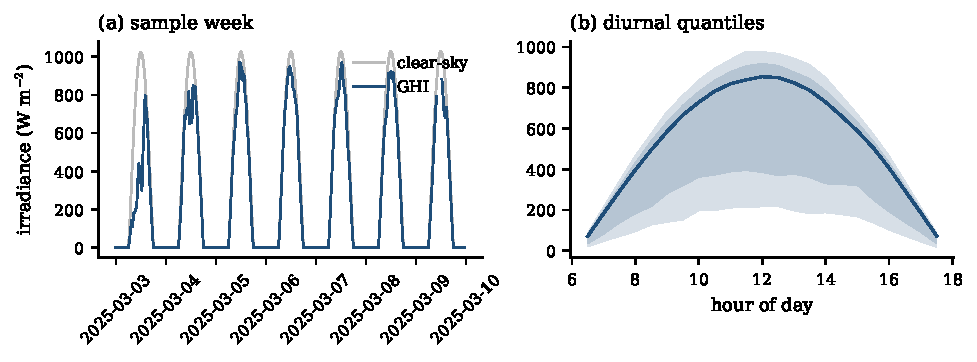
\includegraphics[width=\linewidth]{figures/eda_solar_overview.pdf}
\end{subfigure}\hfill
\begin{subfigure}{0.495\textwidth}
  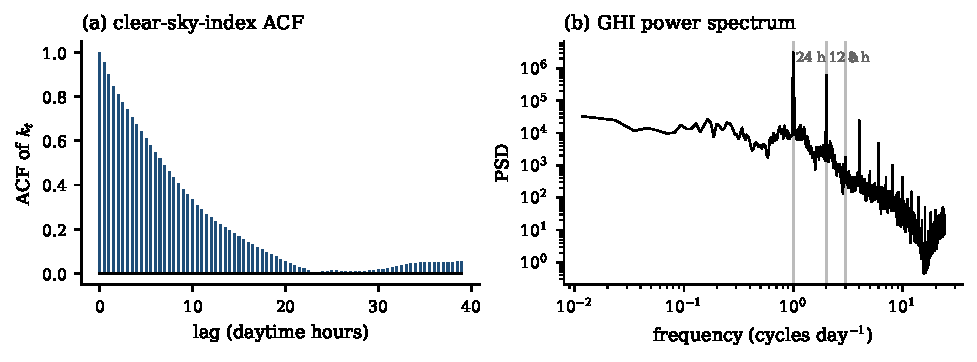
\includegraphics[width=\linewidth]{figures/eda_solar_stats.pdf}
\end{subfigure}
\caption{Solar surrogate EDA (from \code{eda.py}). Left pair: a sample week
of GHI against the clear-sky curve, and the diurnal quantile fan. Right
pair: daytime autocorrelation of $k_t$, and the GHI Welch spectrum with
diurnal harmonics marked. Simulation on surrogate data.}
\label{fig:eda-solar}
\end{figure*}

\subsection{System load (surrogate, GEFCom-like)}
\label{sec:load-dive}

\emph{Construction.} Three years of hourly system load: a double-peaked
diurnal profile, weekday/weekend distinction (weekend factor $0.86$), annual
seasonality, a linear cooling-degree-day (CDD) temperature response of
$55\,\mathrm{MW/^\circ C}$ above the comfort threshold, AR(1) residuals, and
eleven holiday days per year at factor $0.88$.

\emph{Statistics.} Mean $4280$\,MW, s.d.\ $542$, range $2647$--$5618$,
skewness $-0.10$; correlation with coincident temperature $0.64$ and with CDD
$0.63$ --- the canonical load--weather coupling that makes exogenous inputs
mandatory for competitive load
forecasting~\citep{hong2016load,hong2016gefcom}.

\emph{Temporal structure (Figure~\ref{fig:eda-load}).} The autocorrelation
shows the double comb at $24$\,h and $168$\,h --- daily and weekly cycles ---
persisting essentially undamped across the eight-day window: load is the
opposite of solar, a \emph{long-memory, strongly periodic} series where
calendar features do most of the work and the residual after calendar and
temperature is the actual forecasting problem. The correlation heat map
(load, lags, temperature, CDD, calendar flags) quantifies the redundancy a
read-out must negotiate. Implications: multivariate encoding (load lag,
temperature, calendar) rather than scalar; memory requirements modest
\emph{after} the calendar is handled classically; the correct QRC posture is
hybrid --- quantum features for the weather-driven residual, classical
features for the calendar --- exactly the Part~VII pipeline.

\begin{figure*}[t]
\centering
\begin{subfigure}{0.495\textwidth}
  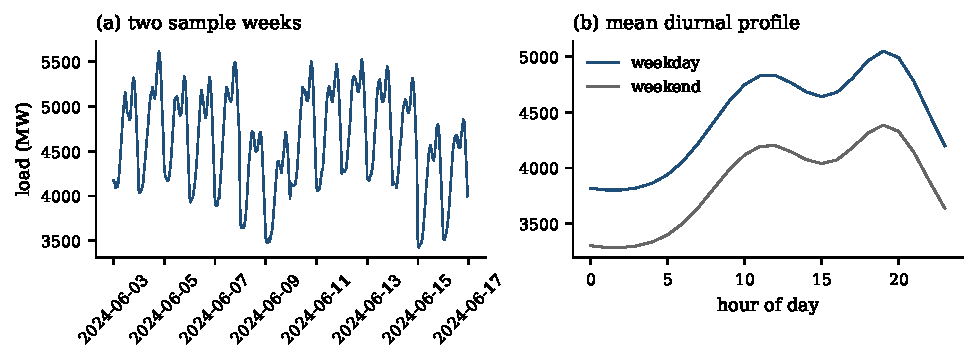
\includegraphics[width=\linewidth]{figures/eda_load_overview.pdf}
\end{subfigure}\hfill
\begin{subfigure}{0.495\textwidth}
  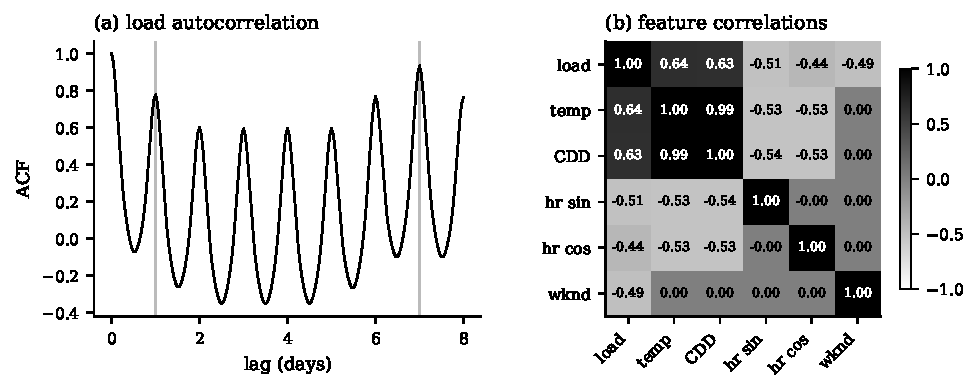
\includegraphics[width=\linewidth]{figures/eda_load_stats.pdf}
\end{subfigure}
\caption{Load surrogate EDA. Left pair: two sample weeks, and weekday versus
weekend diurnal profiles. Right pair: autocorrelation over eight days with
daily/weekly lags marked, and the feature correlation matrix. Simulation on
surrogate data.}
\label{fig:eda-load}
\end{figure*}

\subsection{ENSO sea-surface temperature (real data)}
\label{sec:enso-dive}

\emph{Provenance.} Monthly Ni\~no-region sea-surface temperature, 1950--2010
($n=732$), the NOAA record as bundled with \code{statsmodels}; anomalies are
computed against the monthly climatology, removing the seasonal cycle. This
is the one fully real series in the experiments, and the one with genuine
climate-dynamics content: ENSO is the dominant mode of interannual
variability, with delayed-oscillator dynamics --- coupled ocean--atmosphere
feedback with wave-transit delays --- giving it intrinsic memory and weak
chaos~\citep{suarez1988delayed}.

\emph{Statistics.} SST mean $23.09\,^\circ$C, s.d.\ $2.25$, range
$18.95$--$29.24$. Anomaly: s.d.\ $1.08\,^\circ$C, range $-2.43$ to $+4.60$,
skewness $+1.15$ --- the positive skew is physical (El Ni\~no warm events run
hotter than La Ni\~na events run cold) and any model evaluated only on MSE
will under-serve exactly the strong-event tail that matters.

\emph{Temporal structure (Figure~\ref{fig:eda-enso}).} The anomaly
autocorrelation decays over roughly $12$--$18$ months with a weak negative
lobe near $24$ months --- the oscillator signature; the variance-preserving
spectrum $f\,S(f)$ concentrates power in the $2$--$7$ year ENSO band.
Implications: memory of a year-plus is \emph{required}, which is precisely
why the windowed ($L=8$ months) feature map of Part~IV loses to the recurrent
reservoir here and why this series, small as it is, is the document's
sharpest architectural discriminator. The known hard cases --- the
spring predictability barrier, event-magnitude asymmetry --- make ENSO
indices a permanently honest benchmark: decades of classical effort define
what ``good'' means.

\begin{figure*}[t]
\centering
\begin{subfigure}{0.495\textwidth}
  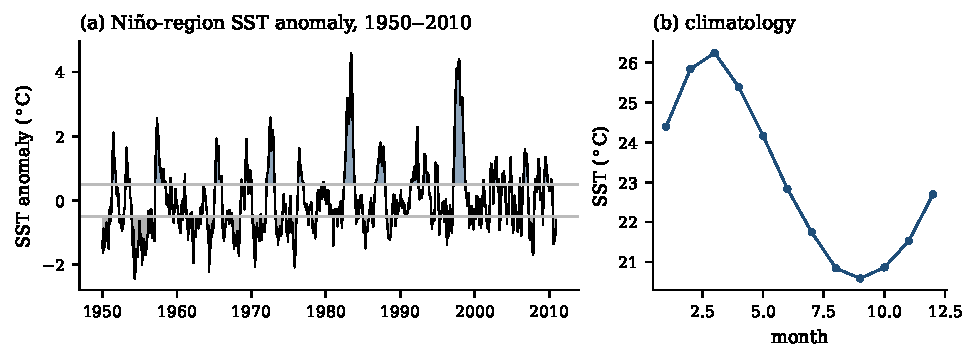
\includegraphics[width=\linewidth]{figures/eda_enso_overview.pdf}
\end{subfigure}\hfill
\begin{subfigure}{0.495\textwidth}
  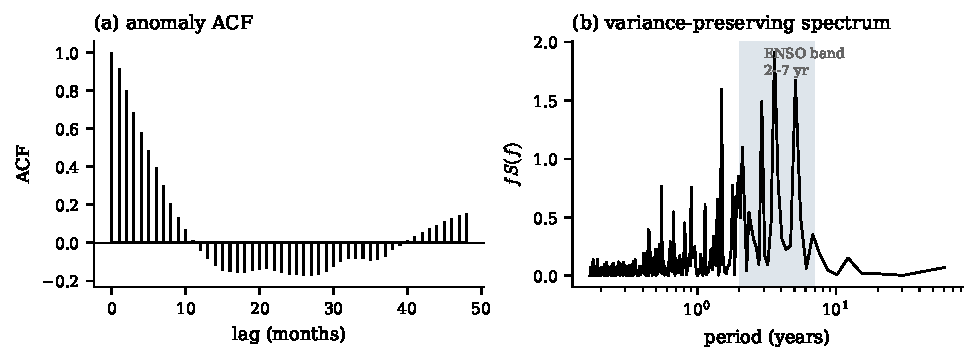
\includegraphics[width=\linewidth]{figures/eda_enso_stats.pdf}
\end{subfigure}
\caption{ENSO EDA (real data). Left pair: the anomaly series with
$\pm0.5\,^\circ$C event shading, and the monthly climatology. Right pair:
anomaly autocorrelation over 48 months, and the variance-preserving spectrum
with the 2--7-year band marked.}
\label{fig:eda-enso}
\end{figure*}

\parttitle{VII}{End-to-End Forecasting Pipelines}

\section{One pipeline, three tasks}
\label{sec:pipeline-spec}

The three application tasks of Part~VI differ in physics but not in shape:
every competent forecasting study, quantum or classical, traverses the same
nine stages, and this part specifies them once so that the task walkthroughs
of Section~\ref{sec:walkthroughs} can be read as three instantiations of one
object rather than three recipes. The stages, with the discipline attached to
each: \emph{(1)~acquisition} --- source, licence, version pinned
(Table~\ref{tab:datasets}); real versus surrogate declared in every caption
downstream. \emph{(2)~quality control} --- gaps located and \emph{masked, not
filled} unless the fill is itself validated; outages longer than the
autocorrelation time split the series rather than bridging it.
\emph{(3)~target transform} --- forecast the variable the physics makes
stationary ($k_t$, not GHI; anomaly, not SST; residual-after-calendar, not
raw load), because every baseline and error metric inherits this choice.
\emph{(4)~encoding} --- scale inputs to the encoding's natural domain
($[0,1]$ for state replacement, angle range for rotations) using
\emph{training-set} statistics only; choose scalar re-upload, multi-channel
rotations, or state replacement per Part~III. \emph{(5)~reservoir} --- fix
architecture, size, and operating point ($J\Delta t$, Section~\ref{sec:temporal-edge})
before touching test data; record the seed. \emph{(6)~read-out} ---
ridge with $\lambda$ chosen on a chronological validation block or by GCV
(Section~\ref{sec:ridge}); features standardised by training statistics.
\emph{(7)~uncertainty} --- at minimum, residual-quantile intervals; for
operational credibility, pinball-loss quantile read-outs
(Section~\ref{sec:uncertainty}). \emph{(8)~baselines} --- the full Part~I
battery (mean, persistence, linear lags, size-matched ESN) plus the Haar
control; a missing baseline is a missing result. \emph{(9)~interpretation} ---
error decomposed by regime (clear/cloudy, weekday/weekend, event/quiet), not
just averaged; claims scoped to what was actually run.

\begin{table*}[h]
\centering\small
\caption{Where each pipeline stage lives in the shipped code, per framework
path. Stages 1--3 and 6--9 are classical and shared; the framework choice
affects only stages 4--5 (and how features are estimated).}
\label{tab:stage-map}
\begin{tabular}{@{}lp{3.4cm}p{3.2cm}p{3.2cm}p{3.0cm}@{}}
\toprule
Stage & Reference (NumPy) & Cirq & Qiskit & PennyLane \\
\midrule
1--3 data & \multicolumn{4}{l}{\code{datasets.py} (generators and ENSO loader), \code{eda.py} (QC statistics)} \\
4 encoding & \code{input\_state}, $u\!\in\![0,1]$ & $R_Y(\gamma g_i u)$ re-upload & $R_Y$ re-upload, transpiled & broadcast $R_Y$ window \\
5 reservoir & \code{QuantumReservoir} (exact $\rho$) & frozen brickwork, exact $\ev{O}$ & noisy backend, shots, MCM & frozen \code{StronglyEntangling}\newline\code{Layers} block \\
6 read-out & \multicolumn{4}{l}{ridge via \code{ridge\_fit} / GCV variant (Listing~\ref{lst:qiskit}); identical maths in all paths} \\
7--9 & \multicolumn{4}{l}{\code{experiments.py} (baselines, regime slicing, figures); conventions of Part~I} \\
\bottomrule
\end{tabular}
\end{table*}

\section{Reference experiments}
\label{sec:reference-experiments}

All experiments below run the exact reference reservoir
(Section~\ref{sec:reference-impl}) at the shipped configuration --- $n=5$
qubits, $V=4$ virtual nodes, disordered Ising couplings $J=1$, field $h=1$,
seed $7$, thirty features --- with every baseline evaluated at the same feature
count. Everything is \emph{simulation}; solar and load data are
\emph{surrogates}; ENSO is \emph{real}. The scripts print every number quoted.

\subsection{Choosing the operating point: the temporal edge}
\label{sec:temporal-edge}

The one reservoir hyperparameter with no classical analogue intuition is the
injection interval $\Delta t$: how much unitary scrambling the register
undergoes between inputs. Figure~\ref{fig:temporal-edge} sweeps
$J\Delta t$ over $2.5$ decades on NARMA-10. The dependence is strongly
non-monotonic: at $J\Delta t \le 0.25$ the propagator is near identity, the
virtual-node features are nearly collinear, and the model cannot beat the
mean predictor (NMSE $\approx 1.05$); performance improves steeply to a
minimum of $0.283$ at $J\Delta t = 1$; beyond it, over-scrambling degrades
the features to a saturation plateau around $0.6$--$0.75$ for
$J\Delta t \ge 4$. This is the \emph{temporal} edge of
\citet{kobayashi2026edge} reproduced in a five-qubit Ising register: their
analysis identifies two independent optima --- a parametric edge, where the
Hamiltonian sits near the boundary between regular and chaotic level
statistics, and a temporal one, where information injected per step is
scrambled enough to mix into the register but not so much that it
thermalises before read-out --- and prescribes exactly this sweep as the
design procedure. Two practice notes. The optimum is task- and
input-scaling-dependent (Section~\ref{sec:edge-of-chaos}): re-sweep when
either changes. And on hardware the sweep is cheap relative to everything
else, because it reuses the same circuits with a rescaled evolution time ---
there is no excuse for publishing at an arbitrary $\Delta t$.

\begin{figure*}[t]
\centering
\begin{minipage}{0.48\textwidth}
  \centering
  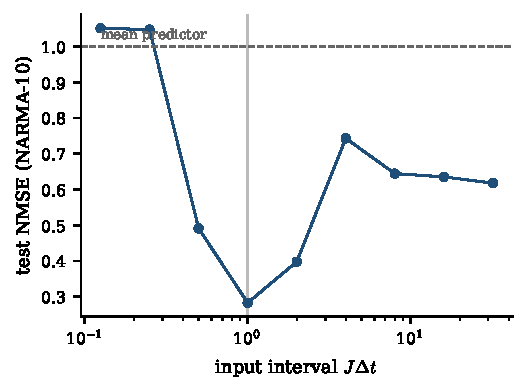
\includegraphics[width=0.98\linewidth]{figures/temporal_edge.pdf}
  \caption{Test NMSE on NARMA-10 versus injection interval $J\Delta t$
  (exact simulation; log axis). The minimum at $J\Delta t=1$ is the temporal
  edge; the dashed line is the mean predictor.}
  \label{fig:temporal-edge}
\end{minipage}\hfill
\begin{minipage}{0.48\textwidth}
  \centering
  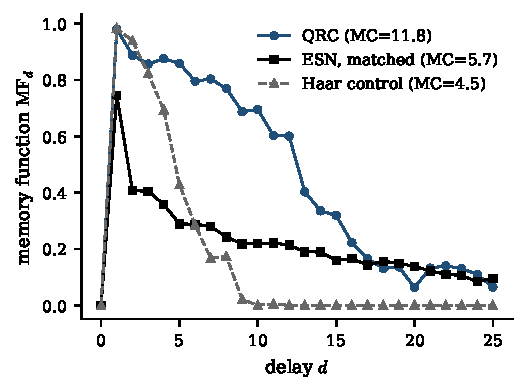
\includegraphics[width=0.98\linewidth]{figures/memory_capacity.pdf}
  \caption{Memory function $\mathrm{MF}_d$ versus delay for the QRC at its
  operating point, the size-matched ESN, and the Haar-random control
  (exact simulation, i.i.d.\ input).}
  \label{fig:memory-capacity}
\end{minipage}
\end{figure*}

\subsection{Memory capacity}
\label{sec:mc-experiment}

At the chosen operating point, Figure~\ref{fig:memory-capacity} shows the
delay-resolved memory function (Eq.~\eqref{eq:mc}, delays to $25$). Total
capacities: QRC $11.8$; size-matched ESN $5.7$; Haar-random control $4.5$.
Two honest readings. First, the \emph{structured} reservoir at its edge
retains linearly recoverable input over roughly twice the delay range of
either control --- and the gap to the \emph{Haar} control specifically shows
this is a property of the tuned dynamics, not of ``being quantum'': a random
unitary of the same size, same observables, same read-out remembers less
than half as much. Second, MC is a diagnostic, not a score: it is measured
on i.i.d.\ input, weights all delays equally, and says nothing about
nonlinearity; the NARMA-10 column below, not this figure, is the performance
claim.

\subsection{Task demonstrations}
\label{sec:task-demos}

Figure~\ref{fig:prediction-demos} shows test-span trajectories for the three
tasks; Table~\ref{tab:results-master} is the complete score sheet.

\begin{figure*}[t]
\centering
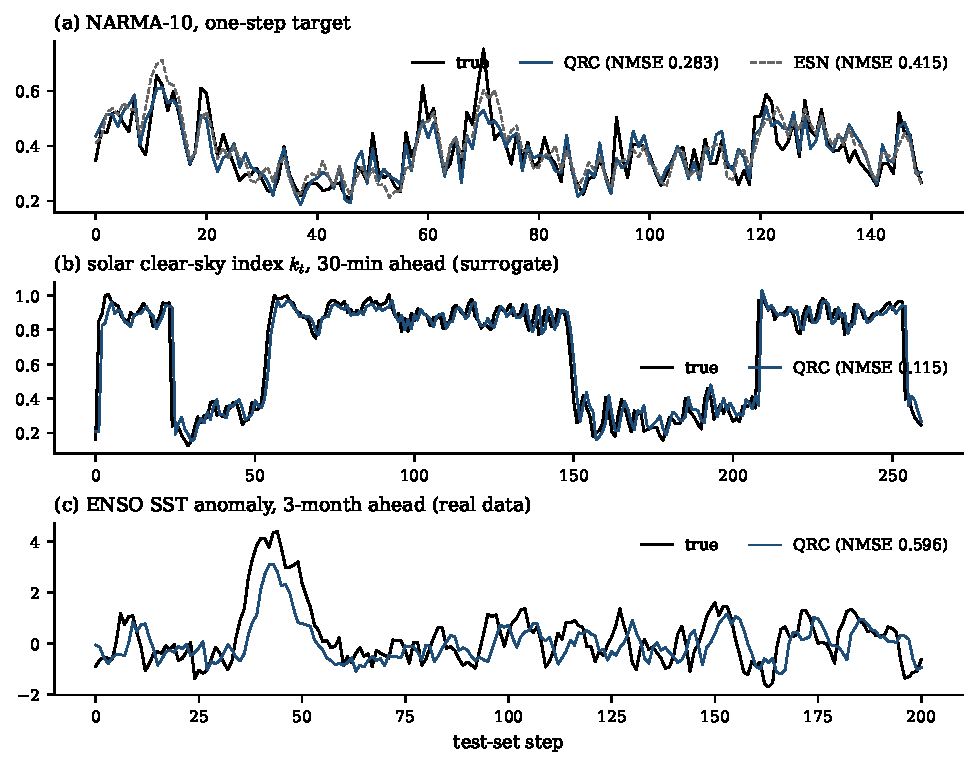
\includegraphics[width=0.92\textwidth]{figures/prediction_demos.pdf}
\caption{Test-span predictions (exact simulation of the reservoir).
(a)~NARMA-10 with QRC and size-matched ESN overlaid; (b)~solar clear-sky
index one step ahead (surrogate data); (c)~ENSO SST anomaly three months
ahead (real data). NMSE values in the legends match
Table~\ref{tab:results-master}.}
\label{fig:prediction-demos}
\end{figure*}

\begin{table*}[t]
\centering\small
\caption{Master results table: test NMSE, exact-expectation simulation,
thirty features for all feature-based models, chronological splits. Bold
marks the best model per task. ``---'' = not applicable.}
\label{tab:results-master}
\begin{tabular}{@{}lccc@{}}
\toprule
Model & NARMA-10 & Solar $k_t$, 1 step (surrogate) & ENSO anomaly, 3 mo (real) \\
\midrule
QRC (Ising, edge) & \textbf{0.283} & 0.115 & 0.596 \\
ESN, size-matched & 0.415 & 0.116 & \textbf{0.555} \\
Haar control & 0.872 & --- & --- \\
Linear lags & 0.740 & \textbf{0.113} & 0.567 \\
Persistence & --- & 0.120 & 0.690 \\
Mean predictor & 1.000 & 1.000 & 1.000 \\
\bottomrule
\end{tabular}
\end{table*}

Reading the table with Part~VIII's eyes. \emph{NARMA-10}: the QRC beats the
size-matched ESN by $32\%$ and the Haar control by $3\times$ --- the designed
benchmark result, on the synthetic task built to reward
memory-plus-nonlinearity, consistent with the small-register literature
\citep{fujii2017harnessing,kutvonen2020optimizing}. \emph{Solar, one step}:
four models within $\pm3\%$ of each other and of persistence --- a statistical
tie. The honest conclusion is that 30-minute-ahead $k_t$ at this site
carries almost no exploitable nonlinear structure beyond its last value, and
\emph{no method}, quantum or classical, adds value here; a study reporting
only the QRC column would look publishable and would mislead.
\emph{ENSO, three months}: every reservoir beats persistence decisively
(memory helps), the tuned ESN leads, and the QRC trails it by $7\%$ --- a
genuinely informative defeat, in two ways. It quantifies the cost of the
window-free but small quantum register on a long-memory task, and against
Part~IV's windowed quantum map on the identical task ($0.747$) it isolates
\emph{recurrence itself} as worth $20$ points of NMSE --- the architectural
conclusion this document considers its most transferable.

\subsection{The shot budget}
\label{sec:shot-budget}

Figure~\ref{fig:shot-noise} replays the NARMA-10 task with the exact
features replaced by finite-shot estimates (eight noise seeds per point).
The analytic ceiling is $0.283$; the sampled model reaches $0.90$ at
$S=10^2$, $0.64$ at $10^3$, $0.53$ at $10^4$, and $0.45$ at $10^5$ ---
converging as $S^{-1/2}$ but still $60\%$ above ceiling at a hundred
thousand shots per feature. The arithmetic this implies for hardware is the
useful output: at thirty features and, say, $S=10^4$, one time step of the
restart protocol costs $3\times10^5$ measured circuits (times the window
length), so a two-thousand-step training series is a $10^9$-shot
commitment --- weeks of queued device time at current throughputs, for a task
a laptop solves exactly in seconds. This is not an argument against hardware
experiments; it is the argument for \emph{small} $T$, batched jobs
(Part~IV), shot-efficient observables, and for treating the eigentask
analysis of \citet{hu2023tackling} and shot-optimal training of
\citet{ahmed2025optimal} as required reading before any device campaign.

\begin{figure*}[t]
\centering
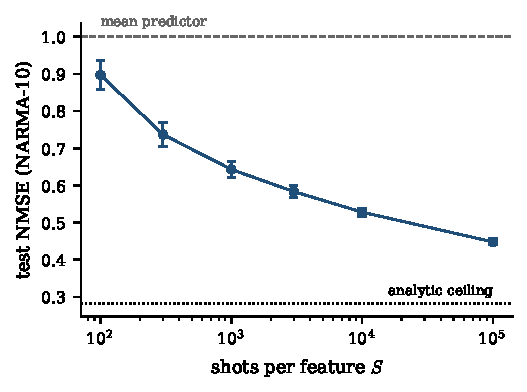
\includegraphics[width=0.5\textwidth]{figures/shot_noise.pdf}
\caption{Shot-noise study on NARMA-10: test NMSE versus shots per feature
$S$ (mean $\pm$ s.d.\ over eight sampling seeds), against the exact-feature
ceiling (dotted) and the mean predictor (dashed). Simulation.}
\label{fig:shot-noise}
\end{figure*}

\section{Task walkthroughs}
\label{sec:walkthroughs}

\subsection{Solar: 30-minute clear-sky index}
\label{sec:pipeline-solar}

\emph{Stages 1--3.} Surrogate NSRDB-like series (real deployment: NSRDB site
extraction, or SURFRAD for minute-scale work); gaps masked ($1.6\%$, longest
$5.5$\,h --- split, never bridge); target $k_t$ per Eq.~\eqref{eq:kt},
daytime only (elevation $>5^\circ$), so the diurnal cycle never inflates
skill. \emph{Stage 4.} Scalar $k_t$, clipped to $[0,1.2]$ then affinely
mapped to $[0,1]$ by training-set range, state-replacement encoding.
\emph{Stage 5.} Reference reservoir at $J\Delta t = 1$. \emph{Stage 6.}
Ridge, $\lambda$ by validation block within the training year.
\emph{Stage 7.} Residual quantiles by cloud regime. \emph{Stage 8--9.}
Table~\ref{tab:results-master}: statistical tie with persistence --- reported
as such. Where a quantum study of this task could still earn its keep, per
the EDA: not the one-step average, but ramp events (regime transitions) and
$2$--$6$\,h horizons where persistence collapses; that is a different target
(Stage~3) and a harder benchmark (event-based scores,
Section~\ref{sec:uncertainty}), and it is listed as research direction R7 in
Part~VIII.

\subsection{Load: day-ahead hourly demand (specified design)}
\label{sec:pipeline-load}

This pipeline is \emph{specified} against the surrogate's EDA but not run in
\code{experiments.py}; it is included because its structure --- the hybrid
posture --- is the one most applications should copy, and it is the natural
first project for a reader (Part~VIII, R6). \emph{Stages 1--3.} GEFCom-like
hourly load with coincident temperature (real deployment: GEFCom2014 load
track, ENTSO-E, or OPSD); target is the residual after a classical
calendar model (hour-of-week means, holiday factor), because
Figure~\ref{fig:eda-load} shows the calendar explains most variance and no
quantum resource should be spent relearning a lookup table.
\emph{Stage 4.} Multi-channel rotation encoding: residual lag, temperature,
CDD --- three channels onto five qubits with fixed random gains.
\emph{Stage 5.} Reference reservoir; re-sweep $J\Delta t$ (the residual's
autocorrelation differs from NARMA's). \emph{Stage 6.} Hybrid read-out:
quantum features concatenated with the calendar prediction and lags ---
Part~IV's Qiskit read-out shape, with the classical-only ablation mandatory.
\emph{Stage 7.} Pinball-loss quantiles, the GEFCom
standard~\citep{hong2016gefcom}. \emph{Stages 8--9.} Success criterion
declared in advance: beat the calendar-plus-linear model on weather-driven
residuals, by regime; anything else is decoration.

\subsection{ENSO: three-month anomaly}
\label{sec:pipeline-enso}

\emph{Stages 1--3.} Real NOAA monthly SST (statsmodels copy pinned);
anomaly against monthly climatology computed from training years only ---
computing climatology on the full record is a subtle leak. \emph{Stage 4.}
Scalar anomaly min--max mapped to $[0,1]$ on training range,
state replacement. \emph{Stage 5.} Reference reservoir; recurrence is the
point (Section~\ref{sec:task-demos}) --- windowed encodings need
$L \gtrsim 18$ months before they stop losing to the recurrent register.
\emph{Stage 6.} Ridge; with $n=732$ months total, the validation block is
thin --- GCV is the stable choice. \emph{Stage 7.} Event-conditional errors:
skill on $|{\rm anomaly}|>0.5\,^\circ$C months reported separately, because
the $+1.15$ skew means MSE under-weights exactly the warm events that
matter. \emph{Stages 8--9.} Table~\ref{tab:results-master}: beats
persistence, trails the tuned ESN --- stated plainly; the residual research
question (can coherence-era registers close the recurrent-memory gap at
matched read-out?) is R2 in Part~VIII.

\section{Uncertainty and evaluation beyond point NMSE}
\label{sec:uncertainty}

Operational forecasting is probabilistic, and the read-out's linearity makes
the upgrade nearly free: replacing the squared loss by the pinball loss at
quantile $\tau$,
$\ell_\tau(e) = \max(\tau e, (\tau-1)e)$ with $e = y - \hat y$,
turns the same feature matrix into a quantile regression, one convex problem
per $\tau$ --- the evaluation standard of the energy-forecasting
community~\citep{hong2016gefcom,hong2016load}. Two further metrics are
attached to the walkthroughs above because averages hide the value:
\emph{regime-conditional} NMSE (clear/cloudy; weekday/weekend;
event/neutral), and \emph{event-based} scores --- hit/false-alarm rates for
solar ramps and warm-ENSO exceedances --- the frame in which extreme-event
reservoir work is already cast~\citep{ahmed2024prediction}. A model that
merely matches a baseline on average but improves the event tail would be
operationally valuable and invisible to Table~\ref{tab:results-master};
none of the models above demonstrated that here, and the claim is left where
it belongs, as an open, testable target.

\parttitle{VIII}{Design Principles and Research Directions}

\section{Design principles}
\label{sec:design-principles}

Ten principles condense Parts~I--VII. Each is stated as an imperative with
its justification and the place in this document where it was earned.

\emph{D1 --- Name your contraction.} Every working reservoir has an explicit
mechanism that erases initial conditions and the remote past: a partial
trace, a reset, engineered dissipation, a window truncation. State which one
your design uses, verify it numerically (trajectory convergence from
different $\rho_0$; PTM spectral radius), and check it contracts toward an
\emph{input-sensitive} region rather than the maximally mixed state
(coherence influx, Section~\ref{sec:quantum-esp}). Architectures that
inherit stability from unexamined device noise are not reproducible across
calibration cycles (Sections~\ref{sec:arch-dissipative}, \ref{sec:hw-ibm}).

\emph{D2 --- Sweep the operating point.} The injection interval and dynamical
regime are not defaults but the reservoir's most sensitive dials; the
temporal-edge sweep of Section~\ref{sec:temporal-edge} moved NARMA-10 error
by a factor of nearly four at fixed architecture. Re-sweep when the task,
input scaling, or noise level changes; on hardware the sweep reuses circuits
and is cheap (Figure~\ref{fig:temporal-edge};
\citealp{kobayashi2026edge,martinez2021dynamical}).

\emph{D3 --- Budget features, not qubits.} The read-out sees $K$ measured,
well-conditioned directions, not $4^n-1$ abstract ones. Track effective rank
and memory capacity of the actual feature matrix; enrich observables
($X$, $ZZ$) and multiplex before adding qubits
(Sections~\ref{sec:extraction}, \ref{sec:cirq}; Table~\ref{tab:cirq-sweep}).

\emph{D4 --- Treat the encoding scale as physics.} Rotation encodings place
the model's approximation power on a frequency comb set by the scale
$\gamma$ \citep{schuld2021effect}; the wrong scale wastes the register on
harmonics the task lacks. The single largest error reduction in Part~IV came
from halving $\gamma$, and the cheapest gradient in the document was the one
tuning it (Sections~\ref{sec:cirq}, \ref{sec:pennylane}).

\emph{D5 --- Anchors before experiments.} Build the validation suite first:
identities with known answers (injection rebuild, unitarity, ridge recovery,
NMSE of the mean $=1$, shot-noise scaling). Every later anomaly is then
attributable in minutes rather than days
(Section~\ref{sec:validation-suite}).

\emph{D6 --- Shots are the currency.} Measure the exact ceiling before any
sampled result; report $S$ next to every number; budget mitigation
multipliers explicitly; and read \citet{hu2023tackling} and
\citet{ahmed2025optimal} before a device campaign. A method that needs
$10^5$ shots per feature to approach its own ceiling has stated its cost
(Sections~\ref{sec:shot-practice}, \ref{sec:shot-budget}).

\emph{D7 --- The baseline battery is part of the model.} Mean, persistence,
linear lags, size-matched ESN, Haar control; chronological splits; the
physically stationary target ($k_t$, anomaly, residual). Part~VII's solar
row exists to show how publishable a meaningless result can look when the
battery is absent (Sections~\ref{sec:baselines}, \ref{sec:task-demos}).

\emph{D8 --- Default to the hybrid posture, with ablations.} Concatenate
quantum features with the cheap classical ones and report quantum-only and
classical-only columns; the difference is the measured quantum
contribution. Part~IV's noisy hybrid \emph{underperforming} its classical
ablation is exactly the kind of result this posture is designed to surface
(Sections~\ref{sec:arch-hybrid}, \ref{sec:qiskit-results}).

\emph{D9 --- Respect concentration and symmetry at scale.} Monitor feature
variance and effective rank as $n$, depth, or noise grow; expect exponential
signal collapse in scrambling or noise-dominated regimes and design against
it (shallow steps, local observables, spatial multiplexing); resolve
symmetry sectors before trusting chaos diagnostics or observable choices
(Section~\ref{sec:concentration};
\citealp{sannia2025exponential,xiong2025role,mcclean2018barren}).

\emph{D10 --- Scope every claim.} Theory, simulation, or hardware; surrogate
or real; the phrase ``quantum advantage'' only behind a controlled scaling
comparison that includes cost. The defensible current claim for QRC in this
domain is parameter-parity plus engineering fit, and this document says no
more anywhere (frontmatter; Section~\ref{sec:arch-comparison}).

\section{Detecting real quantum utility}
\label{sec:detecting-utility}

A benchmark that could in principle certify a quantum benefit has five
properties, and their absence diagnoses most overclaims. \emph{Matched
read-out capacity}: classical baselines get the same number of trained
parameters and comparable tuning effort. \emph{Structure controls}: a
Haar-random quantum reservoir of the same size separates ``tuned dynamics''
from ``being quantum'' (Figure~\ref{fig:memory-capacity}); an efficiently
simulable quantum control (Gaussian or Clifford reservoir) separates
``quantum hardware'' from ``quantum formalism''
\citep{nokkala2021gaussian,gotting2023exploring,palacios2024role}.
\emph{Scaling curves, not points}: performance versus size, shots, and data
on both sides, since crossings, not gaps at one configuration, are the
object of interest. \emph{Cost on the axis}: wall-clock, shots, and energy;
Section~\ref{sec:shot-budget}'s arithmetic belongs in every hardware paper.
\emph{Pre-registered success criteria}: the target, metric, split, and
baselines fixed before the test set is touched --- the cheapest and most
neglected of the five.

\section{Research directions}
\label{sec:research-directions}

Ten directions follow, ordered roughly by increasing ambition. Each gives
motivation, background, a concrete route, difficulty, data, metrics, and
publication potential. All are scoped so that a small group with the shipped
code and modest cloud access can start immediately.

\subsection*{R1 --- A temporal-edge atlas across architectures}
\emph{Motivation:} D2 is currently a per-study ritual; a systematic map
would make it a lookup. \emph{Background:}
\citet{kobayashi2026edge} establish the two-edge (parametric, temporal)
structure for SYK-class reservoirs; Part~VII reproduced the temporal edge in
a 5-qubit Ising register. \emph{Route:} sweep $(J\Delta t$, disorder,
task-memory-length$)$ across the Part~III templates (Ising, chain,
brickwork circuit) at $n\le 12$ exact, correlating optima with level-spacing
ratio and PTM gap; deliver a design chart and the sweep harness.
\emph{Difficulty:} low--medium (compute-bound, conceptually clean).
\emph{Data:} NARMA family, solar $k_t$, ENSO. \emph{Metrics:} NMSE surfaces;
optimum-location predictors. \emph{Potential:} strong methods paper
(PRApplied/PRResearch class); immediately useful tooling.

\subsection*{R2 --- Closing the recurrent-memory gap on ENSO-class tasks}
\emph{Motivation:} Part~VII's sharpest result --- recurrence worth 20 NMSE
points over windowed maps, tuned ESN still ahead of the small register.
\emph{Background:} memory-augmented hybrids \citep{settino2025memory},
feedback reservoirs \citep{kobayashi2024feedback}, NISQRC's
coherence-independent memory \citep{hu2024overcoming}.
\emph{Route:} implement feedback and memory-augmented variants on the exact
simulator; identify which mechanism closes the gap to the matched ESN at
fixed feature count; then a small hardware run (mid-circuit reset, Part~IV
Part-B shape) on the real ENSO series. \emph{Difficulty:} medium--high.
\emph{Data:} ENSO (real); Ni\~no 3.4 from reanalysis for length.
\emph{Metrics:} NMSE and warm-event skill versus matched ESN.
\emph{Potential:} first honest hardware benchmark on a real climate index;
high.

\subsection*{R3 --- Shot-optimal read-outs for forecasting}
\emph{Motivation:} Section~\ref{sec:shot-budget}'s arithmetic is the
adoption barrier. \emph{Background:} eigentask construction
\citep{hu2023tackling}; shot-optimal training \citep{ahmed2025optimal}.
\emph{Route:} apply eigentask-weighted observable selection to the solar and
load pipelines; produce NMSE-versus-total-shot-budget frontiers against
naive uniform allocation. \emph{Difficulty:} medium.
\emph{Data:} surrogate then NSRDB/GEFCom. \emph{Metrics:} error at fixed
budget; budget at fixed error. \emph{Potential:} the paper every hardware
group cites in its methods; solid.

\subsection*{R4 --- Event skill: ramps and extremes}
\emph{Motivation:} Part~VII shows averages are ties; operational value
lives in tails. \emph{Background:} extreme-event reservoir prediction
\citep{ahmed2024prediction}; energy community's event metrics
\citep{hong2016gefcom,inman2013solar}. \emph{Route:} define ramp events on
SURFRAD minute data and warm events on ENSO; train quantile read-outs
(Section~\ref{sec:uncertainty}); compare event-conditional skill (POD/FAR,
tail pinball) across the reservoir battery. \emph{Difficulty:} medium
(metrics discipline is the work). \emph{Data:} SURFRAD (real), ENSO (real).
\emph{Metrics:} event scores, reliability diagrams. \emph{Potential:} high
--- the first tail-focused QRC study in the domain would define the
evaluation standard.

\subsection*{R5 --- Noise as a characterised resource, on hardware}
\emph{Motivation:} D1/D5 versus the reality that device noise drifts.
\emph{Background:} natural reservoirs \citep{suzuki2022natural};
dissipation-as-resource \citep{sannia2024dissipation}; coherence-influx
criterion \citep{kobayashi2024coherence}. \emph{Route:} on one
superconducting backend, characterise the same reservoir circuit across
calibration cycles; correlate task performance with measured
$T_1/T_2$/read-out drift; test the amplitude-damping-helps /
dephasing-hurts prediction by Trotter-inserting engineered channels in
simulation first. \emph{Difficulty:} medium (patience-bound).
\emph{Data:} NARMA + solar surrogate. \emph{Metrics:} performance-drift
curves; influx diagnostics. \emph{Potential:} a reproducibility protocol
the field lacks; solid.

\subsection*{R6 --- The hybrid load benchmark, pre-registered}
\emph{Motivation:} Section~\ref{sec:pipeline-load} is specified but unrun;
it is the cleanest first real-data project. \emph{Background:} GEFCom
practice \citep{hong2016gefcom,hong2016load}; QRC load studies at few-qubit
scale \citep{odo2026quantum}. \emph{Route:} execute the pipeline exactly as
specified (calendar model, residual target, hybrid read-out, ablations,
pinball quantiles) on GEFCom2014 and one ENTSO-E zone; pre-register the
success criterion. \emph{Difficulty:} low--medium.
\emph{Data:} GEFCom2014, ENTSO-E/OPSD (all real).
\emph{Metrics:} pinball loss versus calendar-plus-linear; ablation deltas.
\emph{Potential:} modest novelty, high credibility value --- the reference
others must match methodologically.

\subsection*{R7 --- Solar beyond persistence: multi-horizon, regime-aware}
\emph{Motivation:} the one-step tie (Table~\ref{tab:results-master}) says
move the goalposts to where value exists. \emph{Background:} solar
benchmarking practice \citep{yang2018history,inman2013solar}; hybrid
model-plus-reservoir posture \citep{pathak2018hybrid}.
\emph{Route:} 2--6\,h horizons on NSRDB/SURFRAD $k_t$ with
regime-conditional evaluation; test whether reservoir memory helps most at
regime transitions; optionally fuse a cheap clear-sky/NWP prior.
\emph{Difficulty:} medium. \emph{Data:} NSRDB, SURFRAD (real).
\emph{Metrics:} NMSE by horizon and regime; ramp scores (with R4).
\emph{Potential:} directly relevant to the application community; good
cross-venue paper.

\subsection*{R8 --- Empirical concentration scaling for QRC}
\emph{Motivation:} D9 currently cites theory; design needs measured
curves. \emph{Background:} exponential concentration and symmetry analysis
\citep{sannia2025exponential,xiong2025role}; eigentask noise ceiling
\citep{hu2023tackling}. \emph{Route:} exact simulation to $n=12$--$14$:
feature variance, effective rank, and task NMSE versus $n$, depth, noise
rate, and symmetry sector; fit decay constants; identify the multiplexing
crossover where two $n$-qubit registers beat one $2n$-qubit register at
fixed shots. \emph{Difficulty:} medium--high (careful numerics).
\emph{Data:} NARMA suffices. \emph{Metrics:} scaling exponents; crossover
maps. \emph{Potential:} the quantitative backbone for honest scaling
claims; strong.

\subsection*{R9 --- An analog-platform energy demonstration}
\emph{Motivation:} the largest registers are analog
(Section~\ref{sec:hw-neutral}); the domain lacks any energy-data result on
them. \emph{Background:} 108-qubit Rydberg QRC \citep{kornjaca2024large};
global-detuning encoding's size-independent memory.
\emph{Route:} map a short-window load or ramp \emph{classification} task
(matching the platform's restart/ensemble operation) onto global-detuning
waveforms in emulation; then a partner-hardware run; report against the
full battery including a matched classical kernel.
\emph{Difficulty:} high (platform access and encoding design).
\emph{Data:} GEFCom/SURFRAD-derived labels. \emph{Metrics:} accuracy at
matched trained parameters; shots and wall-clock on the axis.
\emph{Potential:} headline-adjacent if honest; must be pre-registered to
stay so.

\subsection*{R10 --- Clean-physics ESP and edge studies on trapped ions}
\emph{Motivation:} Part~V flags the absence of ion-platform QRC benchmarks
despite the best per-step fidelities and native all-to-all coupling.
\emph{Background:} QCCD mid-circuit primitives \citep{moses2023race};
dynamical-phase reservoir physics
\citep{martinez2021dynamical,kobayashi2026edge}. \emph{Route:} small-$T$,
high-fidelity implementations of the Eq.~\eqref{eq:fn-hamiltonian}
reservoir with mid-circuit reset; measure trajectory-convergence rates
(ESP directly, not via proxy) and the temporal edge on-device; compare with
exact simulation at identical seeds. \emph{Difficulty:} high (access;
shot-rate limits set $T$). \emph{Data:} NARMA-2/10 at small $T$.
\emph{Metrics:} measured contraction rates; edge location on-device versus
simulation. \emph{Potential:} the cleanest hardware--theory comparison
available to the field; high scientific value independent of any advantage
question.

\section{Closing statement}
\label{sec:closing}

This document set out to be the reference its own Part~VIII demands:
theory stated with its assumptions, implementations that run, data
characterised before being forecast, baselines that would embarrass a weak
claim, and research directions scoped to be started rather than admired.
The honest summary of the field it surveys is neither triumphal nor
dismissive. Small quantum registers, operated at their dynamical sweet
spot, demonstrably match classical read-outs several times their size on
memory-nonlinearity benchmarks, and the engineering paths around their two
structural taxes --- measurement statistics and the recurrence gap --- are
active and credible. Whether that matures into practical value for
renewable-energy and climate forecasting is exactly the kind of question
that is settled by pre-registered benchmarks on real data, run by people
who would publish either answer. The code, data discipline, and directions
above are offered to make that settling faster.

\parttitle{IX}{A Staged Repository: From NumPy Reservoir to Product}

This part designs, from scratch, a single repository that carries the whole
programme of this document: a small exact quantum reservoir in NumPy; the same
reservoir expressed as hardware-faithful circuits on an exact simulator; noisy
simulation of a simple Hamiltonian; a battery of more complex Hamiltonians;
qubit-reuse compilation of those Hamiltonians; an independent recurrence-free
reservoir (RF-QRC, Part~X); the integration of RF-QRC with the existing test
architecture and the reuse compiler; and finally the product pipeline of
Part~XI. The repository is not hypothetical: Stages~1--5 already exist as
verified code (the \code{code/} directory shipped with this document and the
companion qubit-reuse package), and the design below states exactly which
files move where, so that assembling the repository is a refactor with green
tests at every step rather than a rewrite.

\section{Design rules the repository inherits}
\label{sec:repo-rules}

Six rules, all earned earlier in this document or in the companion projects,
are promoted from habits to repository law.

\emph{R1 --- Anchors first.} No stage accepts code before its validation
anchors exist and fail meaningfully when sabotaged. The anchor suite of
Part~IV (inject/rebuild identity, propagator unitarity, $\rho$
Hermitian/trace-one/PSD, ridge recovery of a known linear map to $10^{-10}$,
$\NMSE(\text{mean})=1.000$, shot-noise $\sigma \propto S^{-1/2}$) seeds
\code{stage0\_anchors/}, and every later stage appends its own.

\emph{R2 --- The exact reference defines the ceiling.} The NumPy
density-matrix reservoir of Stage~1 is the semantic definition of every
architecture in the repository; framework ports (Qiskit, Cirq, PennyLane) are
validated \emph{against it at identical seeds}, never against intuition.

\emph{R3 --- One endianness point.} Qiskit count keys are little-endian;
\code{counts\_to\_features} performs the single \code{key[::-1]} reversal and
nothing else in the repository may reorder bits.

\emph{R4 --- Printed configuration, fixed seed.} Every experiment script
prints its full configuration block at runtime; \code{SEED = 7} project-wide;
no result enters a table unless a script printed it.

\emph{R5 --- Negative controls are first-class.} The all-to-all
zero-compression rows (SK, SYK$_4$), the Haar-random structureless reservoir,
and the mean-predictor $\NMSE=1.0$ line ship in the same harness as the
headline configurations and appear in the same tables.

\emph{R6 --- Promotion gates, not vibes.} A stage is \emph{done} when its
exit criterion --- a script with an exit code --- passes; downstream stages
import only from stages that are done. The repository's continuous
integration is exactly \code{run\_tests.py} run stage by stage.

\section{The stage ladder}
\label{sec:repo-ladder}

Each stage answers one question and owns one directory.
Table~\ref{tab:repo-stages} summarises; the subsections that follow give the
contents, the entry and exit criteria, and the mapping to existing assets.

\begin{table*}[h]
\centering\small
\caption{The repository's stage ladder. ``Exists'' names verified code that
seeds the stage; new files are set in italics.}
\label{tab:repo-stages}
\begin{tabular}{@{}clp{4.1cm}p{4.6cm}@{}}
\toprule
\# & Question answered & Seed assets & Exit criterion \\
\midrule
0 & do our instruments work? & anchor suites of both codebases & all anchors pass; sabotage test fails \\
1 & exact small-scale QRC (NumPy) & \code{qrc\_core.py}, \code{experiments.py} & NARMA-10/MC results reproduce Part~VII numbers \\
2 & same reservoir as circuits (exact) & \code{qiskit\_qrc\_hw.py}, \code{cirq\_qrc\_minimal.py} & circuit features $=$ NumPy features at seed 7 \\
3 & noisy simple Hamiltonian & Part~IV noise pipeline & noisy-vs-exact degradation curves printed; gate-local caveat stated \\
4 & complex Hamiltonians & seven-family benchmark (reuse repo) & $\langle r\rangle$ diagnostics hit 0.386/0.531 anchors; family scan runs \\
5 & qubit reuse on those & \code{qreuse\_*} (7 modules) & self-calibrated TVD gate; compression table incl.\ zero-compression rows \\
6 & independent RF-QRC & \emph{rfqrc\_reservoir/metrics/ baselines.py}, \emph{mfe\_model.py} & Part~X Phase~0--4 acceptance \\
7 & RF-QRC $\times$ reuse integration & \emph{qreuse\_batch.py} + Stage 5+6 & batch-and-compress validated; width independent of memory horizon \\
8 & product pipeline & \emph{data\_plane/ serving/ decision/ surfaces/ governance/} & Part~XI Phase~8--12 acceptance \\
\bottomrule
\end{tabular}
\end{table*}

\begin{strip}
\begin{lstlisting}[language={},caption={Repository tree. Stages 1--5 are populated by moving verified files; Stages 6--8 are populated by the plans of Parts X--XI.},label={lst:repo-tree}]
qrc-stack/
  README.md                 pyproject.toml            configs/
  run_tests.py              # anchors-first driver; exit 0 iff all stages green
  stage0_anchors/
    test_core_anchors.py    test_reuse_anchors.py     test_rfqrc_anchors.py
  stage1_numpy_core/
    qrc_core.py             baselines.py              tasks.py
    datasets.py             eda.py                    figstyle.py
  stage2_circuits_exact/
    qiskit_qrc_hw.py        cirq_qrc_minimal.py       pennylane_qrc_hybrid.py
  stage3_noisy_simple/
    noise_models.py         exp_tfim1d_noisy.py
  stage4_hamiltonian_battery/
    hamiltonians.py         exp_family_scan.py        # 7 families, <r> dial
  stage5_qubit_reuse/
    qreuse_ir.py            qreuse_analysis.py        qreuse_scheduler.py
    qreuse_compiler.py      qreuse_validation.py      qrc_experiment.py
    exp_reuse_compression.py
  stage6_rfqrc/
    rfqrc_reservoir.py      rfqrc_baselines.py        rfqrc_metrics.py
    mfe_model.py            exp_mfe_extremes.py       exp_lorenz63_check.py
  stage7_integration/
    qreuse_batch.py         exp_rfqrc_reuse.py        exp_vn_fusion_proto.py
    solar_ramps_data.py     exp_solar_ramps.py
  stage8_product/
    data_plane/   connectors.py qc.py transforms.py feature_store.py replay.py
    serving/      feature_provider.py heads.py conformal.py shadow_battery.py
    decision/     stacker.py regime_router.py thresholds.py alerts.py
    surfaces/     api.py dashboard/ agent/            # tools, guardrails, RAG
    governance/   monitors.py promotion_gates.py model_cards.py
  docs/                     # this handbook, regenerated figures
\end{lstlisting}
\end{strip}

\subsection{Stages 0--5: consolidating what exists}
\label{sec:repo-existing}

\emph{Stage 0.} The two anchor suites merge under one driver. The merged
driver keeps the qubit-reuse suite's self-calibration idea --- an equivalence
test passes only if TVD(direct, reuse) $\le 2.5\times$ the shot-noise floor
TVD(direct, direct-rerun) $+\,0.02$ --- and Part~IV's exact-simulation
anchors. A deliberate-sabotage mode (flip the endianness reversal, break a
Kraus normalisation) must turn the suite red; an anchor that cannot fail is
decoration.

\emph{Stage 1.} \code{qrc\_core.py} moves in unchanged: the Fujii--Nakajima
density-matrix reservoir \citep{fujii2017harnessing}, the classical baselines,
and the task generators. Its NARMA-10, memory-capacity, and ENSO numbers
(Part~VII) are the stage's regression targets. The recurrent 5-qubit CZ-ring
ENSO reservoir stays here as the long-memory comparator that Stage~6 must
face honestly.

\emph{Stage 2.} The framework ports (Part~IV) move in with their
validated-against-reference-at-identical-seed tests. This stage owns the
transpilation path (native basis, coupling maps) that makes ``hardware
simulator'' more than a phrase: circuits leave this stage ready for a device
even though this repository runs none.

\emph{Stage 3.} Noisy Aer on the simplest Hamiltonian family (TFIM-1D):
depolarising and thermal-relaxation models, degradation curves versus noise
strength and shots. The stage's documentation carries the caveat this project
measured the hard way: \emph{gate-local noise models cannot see the
$3$--$5\times$ depth inflation that qubit reuse introduces}, so Stage~5
noise claims must never be extrapolated from Stage~3 models alone.

\emph{Stage 4.} The seven-family Hamiltonian battery (TFIM-1D, mixed-field
Ising, XXZ, XY, TFIM-2D, Sherrington--Kirkpatrick, JW-mapped SYK$_4$) with
the disorder dial $W$ and level-spacing diagnostics
\citep{martinez2021dynamical,kobayashi2026edge}; the $\langle r\rangle$
anchors $0.386$ (Poisson) and $0.531$ (GOE) gate the stage.

\emph{Stage 5.} The reuse compiler's seven modules move in unchanged with
their compression scans. The stage's headline artefacts are the
interaction-graph law (nearest-neighbour chains compress $10\to5$ regardless
of gate count; the 2D lattice less; all-to-all not at all) and the
equivalence contract: reuse preserves the \emph{classical measurement
distribution} only --- exactly the contract a QRC read-out needs, and not one
a protocol needing the unmeasured state may assume (DeCross \emph{et al.},
Phys.\ Rev.\ X \textbf{13}, 041057 (2023)).

\subsection{Stages 6--8: the new work}
\label{sec:repo-new}

\emph{Stage 6} implements Part~X Phases~0--4: the recurrence-free reservoir
with virtual-node readout, its metric battery (predictability horizon,
event F-score versus prediction time, VPT, effective rank), the expanded
baseline set (NVAR, QELM ablation, Haar control), and the MFE extreme-event
anchor study, with the Lorenz-63 side check where the classical reservoir is
expected to win at matched degrees of freedom
\citep{ahmed2024prediction,ahmed2025optimal}.

\emph{Stage 7} implements Part~X Phases~5--6: the solar-ramp study on
registry data, the batch-and-compress path through the Stage-5 compiler
(\code{qreuse\_batch.py} lays $B$ independent step circuits side by side with
terminal measurements only, which the existing parser accepts today), the
structural claim that compiled width is independent of memory horizon
(contrast the windowed protocol's measured physical $=T{+}1$), and the
virtual-node fusion prototype behind an IR extension for
measurement-terminated blocks.

\emph{Stage 8} implements Part~XI Phases~8--12: the data plane with its
leakage firewall, the serving core behind the \code{FeatureProvider}
interface, the calibrated decision layer, the product surfaces including the
provenance-guarded agent, and the governance monitors whose promotion gates
are the pre-registered criteria of Parts~X--XI.

\section{Promotion protocol}
\label{sec:repo-promotion}

Work proceeds strictly up the ladder. To promote stage $k$: (i) its anchors
and exit script pass with exit code 0; (ii) its numbers reproduce the
regression targets of the documents that earned them (this handbook for
Stages~1--3, the reuse report for Stages~4--5, Parts~X--XI for Stages~6--8);
(iii) any interface it exports downstream is frozen and versioned; (iv) a
short stage report --- configuration block, tables, honest failures ---
lands in \code{docs/}. Cross-stage experiments (Stage~7 onwards) may only
import frozen interfaces. The repository is \emph{finished} in the same sense
this document is: a stranger rebuilds every figure and table with two
commands, and every claim is scoped theory, simulation, or hardware, with
surrogate data labelled wherever it appears.

\parttitle{X}{Recurrence-Free QRC with Virtual-Node Readout: Theory and Implementation Plan}

This part converts the project's implementation plan for its next
architectural step into the handbook. The plan is exactly that --- a plan:
no result below is claimed, every future number is simulation unless scoped
otherwise, and the success criteria of Section~\ref{sec:rfqrc-prereg} were
fixed before any test data is touched. Notation: in this part the leak rate
of the \emph{classical} feature integrator is written $\varepsilon$
(matching the RF-QRC literature) to avoid collision with the handbook's
classical-reservoir leak $\alpha$; $V$ denotes the fixed random reservoir
unitary.

\section{The architectural improvement, precisely stated}
\label{sec:rfqrc-statement}

The improvement composes three published components, chosen because they
attack the two bottlenecks this project has itself measured: a
memory-horizon-coupled circuit depth, and low effective feature rank.

\emph{(a) Recurrence removal with leaky-integrated classical memory
(RF-QRC).} The windowed restart reservoir of the qubit-reuse experiment
(Stage~5) encodes the last $T$ inputs in one circuit, so the memory horizon
\emph{is} the circuit depth; the compile-time cost was measured directly as
physical qubits $=T{+}1$. RF-QRC \citep{ahmed2024prediction} replaces
in-circuit memory with a classical leaky integrator over measured features
(the input map $\Phi$ is uploaded twice):
\begin{align}
\ket{\psi_k} &= V\,\Phi(u_k)\,\Phi(u_k)\,\ket{0}^{\otimes n},\label{eq:rfqrc-step}\\
r_k &= (1-\varepsilon)\,r_{k-1} + \varepsilon\,\phi(u_k),\label{eq:rfqrc-leak}\\
\hat y_k &= W_{\mathrm{out}}\, r_k,\nonumber
\end{align}
where $\phi(u_k)$ collects the measured features of $\ket{\psi_k}$,
$\varepsilon\in(0,1]$ is the classical leak rate, and $W_{\mathrm{out}}$ is the
ridge read-out. The
circuit now encodes one input (optionally a short window $m\le 3$;
Section~\ref{sec:rfqrc-theory}), its depth is constant in the memory
horizon, and the $T$ per-step circuits are mutually independent ---
embarrassingly parallel, and batchable through the reuse compiler.

\emph{(b) Virtual-node (temporally multiplexed) readout.} Features are
collected at $N_v$ intermediate evolution times $\{t_1,\dots,t_{N_v}\}$
inside the step circuit --- equivalently, the Heisenberg-evolved observables
$\{O(t_i)\}$ are measured \citep{fujii2017harnessing,nakajima2019boosting}:
\begin{equation}
\begin{aligned}
\phi(u_k)&=\big[p(t_1);\dots;p(t_{N_v})\big]\in\R^{N_v 2^n}\\
&\quad\text{or}\quad
\big[\ev{Z_i(t_j)},\,\ev{Z_iZ_l(t_j)}\big]\in\R^{N_v\left(n+\binom{n}{2}\right)}.
\end{aligned}
\end{equation}
In exact simulation the snapshots are free (probabilities at layer
barriers); in shots mode the default realisation is $N_v$ truncated
circuits, with a reuse-fused realisation as a Stage-7 extension.

\emph{(c) Extreme-event evaluation battery and expanded controls.}
Predictability horizon (PH), precision/recall/F-score versus
prediction-time offset, and valid prediction time join NMSE; the baseline
battery gains NVAR (next-generation reservoir computing; Gauthier
\emph{et al.}, Nat.\ Commun.\ \textbf{12}, 5564 (2021)), a QELM ablation
($\varepsilon=1$), and this project's own recurrent reservoirs as
comparators, on top of the standing five (mean $=1.0$ line, persistence,
linear lags, size-matched ESN, Haar-random control).

\section{Theory: why this should work, and where it can fail}
\label{sec:rfqrc-theory}

\subsection{The function class and its honest limitation}
Unrolling Eq.~\eqref{eq:rfqrc-leak} gives a Volterra-like series with an
exponential kernel \citep{boyd1985fading},
\begin{equation}
\hat y_k=\sum_{d\ge 0}\varepsilon(1-\varepsilon)^d\,
W_{\mathrm{out}}\,\phi(u_{k-d}),
\label{eq:rfqrc-unroll}
\end{equation}
which is \emph{additive across delays}: no cross-delay products
$\phi(u_{k-d})\otimes\phi(u_{k-d'})$ appear, although recurrent reservoirs
and NVAR possess exactly those terms and NARMA-$n$ targets contain them
literally. This limitation is not stated in the RF-QRC literature. Two
remedies are kept as switchable ablations: (i) a short in-circuit window
$m\le3$, encoding $(u_k,\dots,u_{k-m+1})$ across qubit groups so the
Born-rule quadratic and the entangler generate cross-delay products within
the window ($m=1$ recovers pure RF-QRC); (ii) a nonlinear read-out head
(degree-2 polynomial or RBF-SVR), offered under a fairness rule to every
classical baseline in the same table. Extreme events may nevertheless sit in
the architecture's sweet spot: turbulent bursts and solar ramps are
threshold-crossing phenomena whose precursors are plausibly low-order
nonlinear functions of a \emph{short} recent window --- the
high-nonlinearity/short-memory corner of the memory--nonlinearity trade-off
\citep{dambre2012information} --- whereas long-nonlinear-memory tasks should
favour recurrence, as this project's own ENSO comparison (recurrent
$\NMSE\approx0.60$ versus windowed $\approx0.75$, Part~VII) already
witnesses.

\subsection{Echo-state property by construction}
\begin{proposition}[Fading memory of the leaky recurrence-free map]
For any input sequence and any $r_0,r_0'$, the states generated by
Eq.~\eqref{eq:rfqrc-leak} obey
$\lVert r_k-r_k'\rVert\le(1-\varepsilon)^k\lVert r_0-r_0'\rVert$.
\end{proposition}
\begin{proof}
The map $r\mapsto(1-\varepsilon)r+\varepsilon\phi(u)$ is affine in $r$ with
Lipschitz constant $(1-\varepsilon)<1$, uniformly in $u$; iterate.
\end{proof}
The echo-state property therefore holds for every $\varepsilon\in(0,1]$,
independent of whether the quantum dynamics is dissipative, unital, or
chaotic --- in contrast with recurrent QRC, whose contraction must be
engineered and verified (PTM spectral radius, coherence influx; Part~II),
and with closed-unitary parameter-encoded reservoirs, which have no fading
memory at all. Washout still discards $N_w$ steps, but only to flush the
classical $r_0$. The kernel $(1-\varepsilon)^d$ makes $\varepsilon$ a pure
memory dial, decoupled from the circuit --- a hyperparameter separation the
recurrent architecture does not offer \citep{jaeger2007optimization}.

\subsection{Capacity and the virtual-node lever}
Total information-processing capacity is bounded by the number of linearly
independent read-out functionals \citep{dambre2012information}; single-time
local-$Z$ readout of $n$ qubits caps them near $n$ regardless of Hilbert
dimension. Virtual nodes raise the cap: the read-out optimises over
$\mathrm{span}\{O(t_1),\dots,O(t_{N_v})\}$, since
$\hat y=\sum_i w_i\tr[\rho_k O(t_i)]=\tr[\rho_k\sum_i w_i O(t_i)]$. The
correlated-spin NMR experiment of arXiv:2508.12383 extracted $653$ features
from nine spins this way and attributes its one-to-two-order NARMA
improvement and its daily-climate result largely to this lever. The caveat
this project has already measured: nominal feature count is not capacity ---
the Stage-5 experiment recorded \emph{effective rank} $\approx2.2$ on a
nominally $2^{12}$-dimensional feature vector under a scalar drive, the
exponential-concentration problem in miniature
\citep{xiong2025role,sannia2025exponential}. The participation ratio of the
feature covariance is therefore a mandatory reported diagnostic, and the
mitigations are modest $n$ (8--11), multichannel encoding, $N_v$ virtual
nodes, and operating below the scrambling regime.

\subsection{Nonlinearity, re-uploading, and the encoding-wrap trap}
The map's nonlinearity stacks the Born-rule quadratic on a truncated Fourier
series in the encoded input whose accessible frequency ladder grows with the
number of data-encoding layers \citep{schuld2021effect}; uploading $\Phi$
twice --- the RF-QRC signature --- doubles the ladder, consistent with the
published ablation in which only the double-upload fully entangling map
matched the recurrent architectures \citep{ahmed2024prediction}. Encoding
gain remains a swept parameter: this project's own sweep found
$\gamma=\pi$ wraps the RX encoding and destroys the linear read-out
($\NMSE\approx1.1$) while $\pi/4$ was selected ($\approx0.03$); the
$\arcsin$ encoding is kept as a wrap-free alternative.

\subsection{Operating point: the two edges}
The inter-node evolution interval $\tau$ (equivalently $J\Delta t$) is swept
log-spaced over at least two decades --- the temporal edge, bounded by the
Thouless time \citep{kobayashi2026edge}; the published $\tau$ sensitivity in
the NMR experiment is this edge in the wild. Where Hamiltonian-evolution
entanglers are used (Stage-4 families), on-site disorder $W$ is the
parametric dial with the $\langle r\rangle$ anchors already unit-tested
\citep{martinez2021dynamical}.

\subsection{Shot noise}
Without recurrence, finite-sampling noise is uncorrelated in time and cannot
compound through a feedback loop --- the mechanism by which sampling noise
degrades recurrent QRC faster \citep{ahmed2025optimal,hu2024overcoming}. The
leak is itself a first-order low-pass filter; on top sit SVD low-rank
truncation of the reservoir matrix and per-feature Savitzky--Golay
filtering, which reduced training loss by roughly two orders of magnitude in
the published hardware runs \citep{ahmed2025optimal}. Standing rule: measure
the noiseless analytic ceiling before any shot study, and report shots and
wallclock next to accuracy.

\subsection{Failure modes kept in view}
(i)~Effective-rank collapse despite $N_v$ (the rank-versus-$N_v$ curve is a
primary figure whatever it shows). (ii)~NVAR dominance at matched feature
count --- RF-QRC without the leak is a random nonlinear feature map of the
current input, so NVAR is its sharpest classical analogue and is absent from
the published comparisons; if it wins, that is the headline.
(iii)~Exogenous stochastic extremes: solar ramps are cloud-advection driven,
so the precursor information may be absent from a univariate series; an
honest null on solar beside a positive MFE anchor is a coherent outcome.
(iv)~Long-memory tasks: an expected loss to recurrence on ENSO, declared in
advance.

\subsection{Fit to the qubit-reuse stack}
\label{sec:rfqrc-reuse-fit}
The compiler's equivalence contract preserves exactly the classical
measurement distribution --- all a QRC read-out consumes. RF-QRC step
circuits have constant depth, so causal cones stay local and the Stage-5
width-scan result (constant physical count for logical $n=8$--$40$) now
holds at \emph{any} memory horizon: the measured pathology physical
$=T{+}1$ disappears because memory moved from a quantum resource to the
classical $\varepsilon$. Batches of independent step circuits carry terminal
measurements only and are parser-legal today; virtual-node fusion ---
$N_v$ truncated circuits joined by measure-and-reset boundaries on one
register --- shares its primitive with the reuse compiler and with
reset-based streaming QRC \citep{hu2024overcoming}, and waits behind an IR
extension for measurement-terminated blocks.

\section{Evidence base}
\label{sec:rfqrc-evidence}

\begin{table*}[h]
\centering\footnotesize
\caption{Published evidence for the adopted components. All are simulation
except where noted; none runs a Haar-random or NVAR control --- the gap this
plan fills.}
\label{tab:rfqrc-evidence}
\begin{tabular}{@{}p{2.9cm}p{3.3cm}p{3.6cm}p{4.6cm}@{}}
\toprule
Source & Model & Task / baseline & Result and caveat \\
\midrule
\citet{ahmed2024prediction} & RF-QRC, double upload, leak & MFE extreme events; tuned size-matched leaky ESN & median PH $8.09$ Lyapunov times at 11 qubits vs classical plateau $\approx5.5$; higher F-score; Lorenz-63 loss reported. Noise-free statevector. \\
\citet{ahmed2025optimal} & RF-QRC $+$ SVD / Savitzky--Golay & shot-noise study; 10 qubits on \code{ibmq\_kyoto} & recurrence-free degrades more slowly under sampling noise; denoising $\sim2$ orders on training loss. Hardware metric is training loss, not PH. \\
arXiv:2508.12383 & 9-spin NMR, natural dissipation, time-multiplexed FID (653 features) & NARMA 2--20; Delhi daily climate vs ESN(500--10000) & NARMA error down 1--2 orders vs prior QRC experiments; temperature $\ge$ ESN(1000), with RBF-SVR head above ESN(10000). Ensemble NMR is backaction-free. \\
C-QRC (Research Square preprint, 2025) & gate-QRC features feeding LSTM/Transformer/XGBoost & solar generation, rolling forecast & gains concentrate in high-volatility and ramp regimes, not average accuracy. Preprint; cite only after audit. \\
\bottomrule
\end{tabular}
\end{table*}

\section{Integration with the existing codebase}
\label{sec:rfqrc-integration}

The compiler modules are untouched; \code{qrc\_experiment.py}'s circuit
builder is refactored into a shared step-circuit factory (the windowed
protocol survives as the \code{recurrent-window} comparator);
\code{counts\_to\_features} remains the single endianness point; the
recurrent CZ-ring of \code{qrc\_core.py} is imported as the long-memory
comparator. New modules are those of repository Stages~6--7
(Listing~\ref{lst:repo-tree}). The configuration surface:

\begin{strip}
\begin{lstlisting}[language=Python,caption={Configuration dataclass, printed at runtime (project convention).},label={lst:rfqrc-config}]
@dataclass
class RFQRCConfig:
    n_qubits: int = 10
    window_m: int = 1            # 1 = pure RF-QRC; 2-3 = short in-circuit window
    n_uploads: int = 2           # RF-QRC signature; 1 = ablation
    entangler: str = "brickwork_zz"   # or "ham_trotter:<family>", "haar_control"
    entangler_layers: int = 2
    gamma: float = np.pi / 4     # swept {pi/4, pi/2, pi}; or "arcsin"
    tau: float = 1.0             # J*dt; swept log over >= 2 decades
    disorder_W: float = 0.0
    n_virtual_nodes: int = 4     # snapshots at uniform layer boundaries
    readout: str = "full_probs"  # or "local_z", "local_zz"
    leak_eps: float = 0.3        # swept log-grid (0.02 .. 1.0]
    shots: Optional[int] = None  # None = exact snapshots
    denoise: str = "none"        # "svd:<k>", "savgol:<w>,<p>"
    ridge_beta: tuple = (1e-6, 1e-9, 1e-12)
    seed: int = 7
\end{lstlisting}
\end{strip}

\section{Phased plan with acceptance criteria}
\label{sec:rfqrc-phases}

\paragraph{Phase 0 --- anchors.} Environment restored and the untouched
suites green; then the new anchors of Table~\ref{tab:rfqrc-anchors}, each
with an exact expected value, appended to \code{run\_tests.py}.

\begin{table*}[t]
\centering\small
\caption{New validation anchors (Phase 0). ``Exact'' entries carry no shot
noise.}
\label{tab:rfqrc-anchors}
\begin{tabular}{@{}llp{5.2cm}@{}}
\toprule
Component & Anchor & Expected \\
\midrule
leak & impulse response & $r_d=\varepsilon(1-\varepsilon)^d$ exactly \\
leak & memory function, iid input & matches analytic form \\
virtual nodes & 2-qubit hand-solved circuit & snapshot probabilities $=\tr[\rho(t_i)P]$ \\
virtual nodes & snapshot vs truncation & identical distributions, TVD $<10^{-12}$ \\
endianness & known basis state & feature ordering matches statevector \\
PH ladder & synthetic ramp series & equals hand computation; ladder terminates \\
F-score & event-free window & degenerate cases handled \\
NVAR & known quadratic map & exact recovery to $10^{-10}$ \\
Haar control & two distinct inputs & distinct features; structure-free \\
NMSE & mean predictor & exactly $1.000$ \\
\bottomrule
\end{tabular}
\end{table*}

\paragraph{Phase 1 --- core module.} \code{rfqrc\_reservoir.py}: shared
step-circuit factory; exact path via statevector snapshots at layer
barriers; shots path via truncated circuits through the existing Aer runner;
leak applied elementwise after multiplex concatenation; washout. Accept:
anchors green; exact versus $10^6$-shot truncation agree within shot noise
on a 4-qubit test.

\paragraph{Phase 2 --- read-out and training.} Ridge with chronological
splits; $\lambda$ by chronological validation block or GCV via SVD when the
tail block is thin; denoisers between features and ridge in shots mode;
optional heads behind the fairness rule. Accept: ridge anchor; one
evaluation harness applies any head to all models.

\paragraph{Phase 3 --- metrics and battery.} PH frozen to the
Racca--Magri convention (criterion
$|k_{\mathrm{pred}}-k_{\mathrm{true}}|/(k_e-\bar k)<0.2$, ladder start
$10\,\mathrm{LT}$, decrement $0.5\,\mathrm{LT}$); F-scores from
$\ge10^3$ starting points binned by prediction-time offset; feature-count
matching rule --- ESN nodes $=$ NVAR features $=$ quantum feature dimension
$N_v F_{\mathrm{step}}$ --- so all read-outs train equally many weights;
effective-rank column mandatory. Accept: battery end-to-end on a synthetic
series, every number printed.

\paragraph{Phase 4 --- MFE anchor study.} Nine-mode MFE shear-flow model,
$\mathrm{d}t=0.25$, $\Lambda=0.0163$ ($1\,\mathrm{LT}\approx61.3$ time
units), ensemble of $2000$ series of $65\,\mathrm{LT}$, laminarised series
discarded ($k>k_l=0.48$), training $25$ series $\times\,20\,\mathrm{LT}$,
test $500$; extreme event $k\ge k_e=0.1$. Sweeps: $n\in\{8,\dots,11\}$,
$N_v\in\{1,2,4,8\}$, $\varepsilon$ log-grid, $\tau$ two-decade log grid,
$\gamma$ set, $m\in\{1,2,3\}$, five seeds; comparators include the
windowed protocol and the recurrent ring. Accept: the qualitative
published finding reproduced or its failure reported; the Lorenz-63 check
run and reported.

\paragraph{Phase 5 --- solar ramp application.} SURFRAD 1-min ground truth
(aggregated to 5-min) primary, NSRDB 30-min secondary; registry vetting in
full; clear-sky index $k_t$ fit on the training span only; masking, never
interpolation. Ramp label $|k_t(t{+}h)-k_t(t)|\ge\rho$ with $\rho$ the
train-span 95th percentile, horizons 30 minutes to 4 hours; direct
multi-horizon multitask read-outs; multichannel encoding across qubit
groups; hybrid posture with quantum-only and classical-only ablation
columns. Known hazard honoured: one-step point forecasting on solar is a
four-way statistical tie with persistence, so event-level metrics are
primary. Secondary honesty check: RF-QRC versus the recurrent ring on ENSO,
expected loss declared. Accept: Section~\ref{sec:rfqrc-prereg} evaluated
once on the untouched test span.

\paragraph{Phase 6 --- reuse integration.} (a)~Batch-and-compress through
the Stage-5 pipeline, gated by the self-calibrated TVD rule; compression
versus entangler topology including the all-to-all negative control;
feature-interchangeability check repeated. (b)~Virtual-node fusion
prototype behind the IR extension, validated blockwise against unfused
truncation. (c)~Shot study, gated on the analytic-ceiling check, with the
cost axis reported. Accept: as stated per item.

\paragraph{Phase 7 --- documentation.} This part and its results enter the
handbook; citation audit before the PDF ships (the C-QRC preprint is cited
only if it verifies); skills updated; handoff written.

\section{Pre-registered success criteria and claim discipline}
\label{sec:rfqrc-prereg}

Fixed before test data is touched; evaluated once. (1)~MFE: median PH of
the best swept configuration at $n=11$ exceeds the size-matched ESN plateau
by $\ge1.0\,\mathrm{LT}$, exceeds the Haar control by
$\ge0.5\,\mathrm{LT}$, and is $\ge$ NVAR at matched feature count; any
clause failing, the corresponding null is the result. (2)~Solar: at
$h=1$ and $2$ hours, hybrid F$_1$ on ramp events exceeds the classical-only
ablation by $\ge0.03$ absolute, quantum-only column reported; secondary
NMSE on $k_t$ with the mean line and persistence row present. (3)~ENSO:
reported, expected recurrence win. Claims permitted on success: event-level
improvement at matched read-out capacity; width-efficiency (constant
compiled width versus memory horizon); simulation-scoped. Claims banned
regardless: quantum advantage or speed-up; hardware implications from Aer;
any number not printed by a script.

\section{Compute and risks}
\label{sec:rfqrc-risks}

Exact simulation to $n=11$ with $N_v$ snapshots is cheap; the MFE ensemble
and the sweep grid dominate (coarse-then-fine pruning). Feature dimensions
up to $N_v 2^n\sim8192$ against $10^3$--$10^4$ training rows: ridge/GCV
suffices, SVD truncation doubling as regularisation. Shots mode multiplies
executions by $N_v$ in the truncated realisation --- exactly the cost the
fusion prototype targets. Principal risks and responses: effective rank
stagnant (report the curve; multichannel encoding is the lever); NVAR wins
(report as headline; value then rests on width-efficiency and the hardware
path); solar null (coherent beside a positive MFE anchor); IR extension
complexity (deferred; batching delivers without it); preprint fails audit
(drop the citation).

\parttitle{XI}{From Pipeline to Product: Extreme-Climate Forecasting for Users}

Part~X delivers a validated forecast core. This part wraps it in the full
system a user would touch --- data plane, hybrid forecast core, decision
layer, product surfaces, personas --- adds implementation Phases~8--12, and
integrates a survey of classical ML/DL and agentic-AI post-processing at the
user boundary. The governance is inherited unchanged: pre-registered
promotion gates, simulation-scoped claims, every number traceable to a run
identifier, and the quantum contribution always reported as a delta against
its own classical ablation.

\section{Product definition}
\label{sec:prod-def}

\emph{Two tracks, routed by measured memory requirements.} Track~A
(operational extremes, minutes to hours): solar irradiance and PV-output
ramp events driven by convective cloud fields, squalls, and haze --- the
extreme-climate signal at operational timescale, and the regime where the
evidence of Part~X locates QRC value; short-memory, high-nonlinearity
targets, served by RF-QRC with virtual nodes. Flagship geography: tropical
convective regimes (Singapore and South-East Asian rooftop and microgrid
PV), where ramps are frequent, steep, and costly. Track~B (tactical and
seasonal extremes, weeks to months): ENSO phase transitions and
anomalous-heat episodes; long-nonlinear-memory targets, served by the
recurrent CZ-ring reservoir whose ENSO advantage this handbook measured
(Part~VII). The Part~X ``ENSO tension'' thereby becomes an
architecture-selection rule rather than an embarrassment.

\emph{Decisions fed and error costs, in writing.} Track~A feeds battery
pre-charge and discharge, spinning-reserve commitment, curtailment, and
intraday positions; a miss costs imbalance penalties, diesel spin-up, or
voltage excursions, while a false alarm costs battery cycling and reserve
over-procurement. Track~B feeds seasonal hedging, maintenance windows,
water and agricultural allocation, and parametric-insurance triggers.

\emph{Incumbents named.} Persistence and smart-persistence (the honest
one-step champion on solar --- this project's own calibration); NWP-derived
vendor forecasts; all-sky-imager nowcast systems, whose published ramp
capture spans roughly $26$--$92\%$ with large false-alarm spreads --- a
genuinely weak incumbent frontier on ramps; and deep-learning weather
models, which the product \emph{consumes} as exogenous channels rather than
competes with. The venture owns three things only: the event-focused hybrid
feature layer, the calibrated decision layer that converts forecasts into
cost-optimal alerts, and the benchmark-governance layer --- the
no-overclaiming discipline packaged as a feature. The quantum module sits
behind an interface: if its pre-registered delta over the classical-only
ablation fails at any promotion review, the product ships classical-only
and the quantum track continues as research. Quantum-optional architecture
is the de-risking posture.

\emph{Why RF-QRC specifically is the productisable QRC.} Recurrent QRC
carries quantum state across steps: inference is stateful, sequential,
non-cacheable, and latency-bound to the quantum backend. RF-QRC step
features depend only on the current quantised input window; memory is the
classical leak. Features are therefore memoisable, per-step computation is
stateless and parallel, and inference latency decouples from the backend.
At product-relevant sizes ($n\le11$) the exact simulator \emph{is} the
production backend --- fast, deterministic, and identical in distribution
to ideal hardware --- while the reuse compiler keeps the hardware path open
for the regime where simulation fails, at compiled widths independent of
memory horizon (Section~\ref{sec:rfqrc-reuse-fit}). This is stated plainly
to users: near-term inference is quantum-inspired simulation; hardware
execution is a scaling option, not a marketing prop.

\subsection{Personas and their contracts}
\label{sec:prod-personas}

Every persona contract names its metric before onboarding --- the
pre-registration discipline applied to customers.

\begin{table*}[h]
\centering\footnotesize
\caption{Personas, decisions, and the metric each contract names.}
\label{tab:prod-personas}
\begin{tabular}{@{}p{2.9cm}p{3.1cm}p{1.7cm}p{2.6cm}p{3.4cm}@{}}
\toprule
Persona & Decision & Horizon & Surface & Metric that matters \\
\midrule
microgrid / island-grid operator & battery and genset scheduling & 15\,min--4\,h & alerts (chat/SMS/webhook), dashboard & ramp F$_1$ at a fixed false-alarm budget; lead time \\
C\&I rooftop energy manager & load shifting, demand-charge avoidance & 30\,min--6\,h & dashboard, weekly digest & avoided cost per month \\
utility control room / VPP & reserve procurement, curtailment & 1--24\,h & API into EMS/SCADA historian & pinball loss on quantiles; recall at capped false-alarm rate \\
energy trader & intraday position vs imbalance & 1--12\,h & API, scenario tool & cost-weighted CRPS; volatility-regime hit rate \\
climate-risk analyst / insurer & parametric triggers, seasonal exposure & weeks--months & reports, API & calibrated exceedance probabilities \\
researcher tier & benchmarking, method development & --- & open harness, feature API & seed-exact reproducibility \\
\bottomrule
\end{tabular}
\end{table*}

\section{End-to-end architecture}
\label{sec:prod-arch}

\begin{strip}
\begin{lstlisting}[language={},basicstyle=\ttfamily\scriptsize,caption={Six-layer architecture. L6 governance spans the whole pipeline.},label={lst:prod-layers}]
L1 INGEST      L2 TRANSFORM        L3 FORECAST CORE       L4 DECISION       L5 SURFACES
SURFRAD/NSRDB  QC (mask, never     classical features     calibration       API (REST/stream)
ERA5 / NOAA    interpolate)        + RF-QRC+VN features   (conformal,       dashboard
site SCADA  -> clear-sky index  -> via FeatureProvider -> isotonic)      -> alert engine
NWP + DL-      k_t (train-span     [sim|hw-batch|cache]   stacker (GBM/     agent assistant
weather feeds  fit, frozen per     quantile+event heads   shallow DL)
(exogenous)    version); anomaly   shadow baseline        regime router
               transforms;         battery (always on)    cost-sensitive
               feature store                              thresholds
        L6 GOVERNANCE: drift + calibration monitors, effective-rank health,
        champion-challenger, promotion gates = pre-registered criteria,
        model cards, run-ID audit log
\end{lstlisting}
\end{strip}

\emph{L1, ingestion and QC.} Connectors per the dataset registry of
Part~VI plus private site feeds; the vetting checklist applies to every new
source; missing data is masked, never silently interpolated; gaps longer
than the autocorrelation time split the series; raw data is immutable and
versioned.

\emph{L2, transform and feature store.} Physics-derived target transforms
(solar to clear-sky index; climate to anomalies against training-years
climatology) live in a transform service holding the frozen train-span
statistics per model version --- the leakage firewall as an architectural
component rather than a code-review hope. Calendar and solar-geometry
features come from lookup: no quantum resource is spent on what a lookup
table solves.

\emph{L3, forecast core.} The Part~X core behind a narrow interface:

\begin{strip}
\begin{lstlisting}[language=Python,caption={The forecast core's only coupling to quantum execution.},label={lst:prod-provider}]
class FeatureProvider(Protocol):
    def features(self, window: np.ndarray, cfg: RFQRCConfig) -> np.ndarray: ...

# SimProvider      exact Aer snapshots (production default, n <= 11)
# HardwareProvider reuse-compiled batched jobs (qreuse_batch -> compile_with_reuse),
#                  gated by the self-calibrated TVD equivalence check as CI
# CachedProvider   memo keyed by (config_hash, quantised window m); valid because
#                  RF-QRC step features are stateless; leak applied downstream
\end{lstlisting}
\end{strip}

Heads on the shared feature stream: multi-horizon quantile read-outs
trained on pinball loss (one $W_{\mathrm{out}}$ per horizon), an
event-probability head, and a per-horizon leak. The shadow battery ---
persistence, smart-persistence, linear lags, size-matched ESN, NVAR, Haar
control, classical-only ablation --- runs on every production window
permanently: champion--challenger is the steady state, not a launch event.

\emph{L4, decision layer.} Calibration wrapper, stacker over the hybrid
feature block, regime router, and cost-sensitive thresholds per persona
cost matrix, emitting alert objects that carry their own provenance and
their delta over persistence:

\begin{strip}
\begin{lstlisting}[language={},caption={Alert object: honesty as payload.},label={lst:prod-alert}]
{ "site": "...", "event": "ramp_down", "horizon_min": 60,
  "p_event": 0.83, "magnitude_q10_q50_q90": [-0.31, -0.22, -0.12],
  "lead_time_min": 47, "regime": "convective_afternoon",
  "conformal_coverage_target": 0.9, "run_id": "2026-07-11T04:20Z#a1b2",
  "model_version": "hybrid-1.3.0",
  "baseline_delta": {"vs_persistence_F1": +0.11} }
\end{lstlisting}
\end{strip}

\emph{L5, surfaces.} REST and streaming API; a dashboard whose benchmark
table is non-removable by design; alert channels; the agent assistant of
Section~\ref{sec:prod-survey-agent}.

\emph{L6, governance.} Input-drift and rolling-coverage monitors; feature
effective rank as a QRC-specific health metric (rank collapse is the
leading indicator that quantum features have degenerated); alert-fatigue
counters; retraining with walk-forward re-validation; promotion between
model versions only through the pre-registered gates.

\section{Implementation Phases 8--12}
\label{sec:prod-phases}

\paragraph{Phase 8 --- data plane.} Registry connectors and one
private-feed adapter; QC service implementing the mask policy with gap
reports; transform service with a frozen-statistics registry keyed by model
version; a light feature store; a walk-forward replay harness driving
everything through the same code path as live inference. Accept:
bit-identical backtest reproduction from raw data with two commands; the
leakage-audit script passes.

\paragraph{Phase 9 --- serving core.} \code{FeatureProvider}
implementations (Sim, Cached; Hardware stub wired through the Stage-5
compiler as CI); quantile and event heads with per-horizon leak; adaptive
conformal wrapper with a rolling-coverage monitor; shadow-battery service;
latency budget of sub-second simulated features at $n\le11$ on a 5-minute
cadence, alerts within 60 seconds of data arrival. Accept: rolling
empirical coverage within three points of target on held-out streams;
battery columns present in every stored prediction row; cache-hit
accounting in logs.

\paragraph{Phase 10 --- decision layer.} Stacker ablation under the
fairness rule (ridge versus gradient boosting versus shallow TCN/LSTM
versus a small transformer, all offered to the classical-only ablation);
regime router (clear-sky classification plus changepoint detection) with
regime-conditional error reporting; a cost-sensitive threshold optimiser
taking the persona cost matrix (expected-cost minimisation, not F$_1$
maximisation); alert engine with deduplication, escalation, and fatigue
caps. Accept: decision-layer value reported in cost units alongside F$_1$;
the stacker table includes the classical-only column, and if the quantum
delta is zero the table says so.

\paragraph{Phase 11 --- surfaces and agent.} API with documentation and
client snippets; dashboard; the assistant of
Section~\ref{sec:prod-survey-agent} with its tool registry
(\code{get\_forecast}, \code{get\_alert\_rationale},
\code{run\_whatif\_backtest}, \code{get\_benchmark\_table},
\code{get\_model\_card}, \code{configure\_site\_draft}), retrieval index
over model cards, run logs, and event post-mortems, the numeric-provenance
guardrail, and the recommend-never-actuate boundary; report generator;
onboarding copilot producing draft site configurations for human approval.
Accept: a grounded-answer evaluation set passes with every numeric claim in
sampled transcripts tracing to a tool call --- zero fabricated numbers
tolerated; time-to-first-alert for a new site under one day.

\paragraph{Phase 12 --- pilot and promotion.} One or two design-partner
sites in shadow mode for at least six weeks against the operator's
incumbent, producing the honest benchmark table; pilot exit criteria
written before the pilot starts (for example, ramp F$_1$ at least the
incumbent's plus $0.05$ at the operator's false-alarm budget, latency SLA
met, zero provenance violations); activation on pass; quarterly promotion
reviews re-running the pre-registered gates, including the contractual
possibility of demoting the quantum feature block. Accept: the pilot
report itself, whatever it says.

\section{Economics and operational honesty}
\label{sec:prod-econ}

The cost axis is reported next to every accuracy number: simulated feature
cost per prediction, cache-hit rate, and --- for any hardware experiment
--- shots and wallclock per prediction; a model needing $10^9$ shots to
match a laptop has answered the business question. Public sources
(SURFRAD, NSRDB, ERA5, NOAA) carry attribution requirements; site SCADA is
private and stays on the customer boundary, with only derived features
leaving if contracted. The degrade-graceful ladder --- quantum features,
then classical-only stacker, then smart-persistence --- keeps the alert
schema identical at every rung, so downgrades are invisible to
integrations.

\section{Survey: classical ML/DL and agentic AI at the post-processing end}
\label{sec:prod-survey}

\subsection{Statistical post-processing}
Raw regression outputs, reservoir or otherwise, are not calibrated decision
inputs. The forecasting tradition supplies the fixes: distributional
regression in the MOS/EMOS lineage, quantile regression on pinball loss,
isotonic recalibration of event probabilities, CRPS as the proper score for
the quantile fan. All are computationally trivial, all sit strictly
downstream of the feature stream, and none care whether the features were
quantum. Adopted: quantile heads plus isotonic recalibration.

\subsection{Conformal prediction: guarantees instead of accuracy claims}
Split and adaptive conformal methods wrap any point or quantile forecaster
and deliver distribution-free finite-sample coverage; adaptive variants
adjust the miscoverage rate online and so track regime shifts. The
strategic fit is exact: the product can contractually promise
``90-percent intervals that cover 90 percent, monitored weekly'' --- a
guarantee --- while accuracy claims remain comparative and scoped.
Adopted: an adaptive conformal wrapper as the default interval layer, with
the rolling-coverage monitor in L6.

\subsection{Machine-learned stackers over hybrid features}
Gradient-boosted trees remain the strongest tabular learners for stacking
heterogeneous blocks: reservoir features, classical lags, calendar and
geometry, NWP and DL-weather channels. The C-QRC preprint is the direct
precedent --- gate-QRC used as a feature extractor feeding LSTM,
Transformer, and XGBoost heads, with the honest finding that gains
concentrate in high-volatility and ramp regimes rather than average point
accuracy. That is this project's thesis stated by an independent group, and
it fixes the stacker's role: event-regime lift, not accuracy everywhere.
Adopted: a gradient-boosted stacker as the default, under the fairness
rule.

\subsection{Deep heads and foundation models: two distinct roles}
Sequence heads (TCN, LSTM, small transformers) are alternative stackers
where horizon-coupled multivariate structure matters, and are evaluated in
the Phase-10 ablation rather than assumed. Time-series foundation models
join the \emph{baseline battery}: if a frozen pretrained forecaster matches
the pipeline on event metrics, the honest table says so. Deep-learning
weather models and classical NWP enter as \emph{exogenous input providers}
--- their gridded forecasts become L2 channels --- because the product's
edge is the event-focused last mile, not global weather modelling. This
division of labour is the survey's central architectural conclusion.

\subsection{Regime-aware routing}
Changepoint and hidden-Markov detectors with clear-sky classification gate
per-regime read-outs and thresholds; regime-conditional error reporting
doubles as the router's evaluation. The Track~A/B architecture routing of
Section~\ref{sec:prod-def} is the same idea one level up: measured memory
requirements select the reservoir.

\subsection{Agentic AI at the user boundary}
\label{sec:prod-survey-agent}
The 2024--2026 literature has converged on language-model agents as the
interpretation and decision-support tier over energy forecasting systems,
not as forecasters. A 2026 review of LLM-agent renewable forecasting
(arXiv:2605.25141) proposes a six-layer taxonomy whose top layers are
uncertainty estimation and natural-language reporting, and names
hallucination control, drift, and EMS interoperability among twelve open
challenges; prototype systems --- GridMind for multi-agent power-system
analysis (arXiv:2509.02494), Grid-Agent for grid control with stepwise
rationales (arXiv:2508.05702), ``Power Agent'' concept papers, and
forecasting-process automation frameworks --- cluster into six patterns, of
which this design adopts five and rejects one:

\begin{enumerate}
\item a conversational analyst over the forecast and metrics store
  (retrieval plus metric tools): questions about yesterday's ramp are
  answered by tool calls whose numbers carry run identifiers ---
  \emph{adopted};
\item an alert triage and explanation agent attaching rationale to each
  alert: regime label, leading feature attributions, retrieved analogue
  past events with outcomes --- \emph{adopted}, and the single
  highest-leverage adoption feature, because operators trust alerts they
  can interrogate;
\item a what-if and scenario agent orchestrating parameterised backtest
  calls (replay a monsoon week under a different alert policy and report
  the cost delta), the decision-theoretic direction of the review
  literature mapped onto the Phase-10 cost matrices --- \emph{adopted};
\item a report and compliance generator drafting persona digests,
  post-event analyses, and re-validation reports from templates and
  tool-fetched numbers --- \emph{adopted};
\item an onboarding copilot translating natural language into a draft site
  configuration for human approval --- \emph{adopted}, the
  easy-to-adopt lever, with time-to-first-alert measured in hours;
\item an autonomous control agent actuating switches or dispatch ---
  \emph{rejected}: the boundary is recommend-never-actuate with a human in
  the loop, and actuation belongs to the customer's EMS and its safety
  case, not to a forecasting vendor's language model.
\end{enumerate}

Guardrails, non-negotiable and recognisably this project's honesty
discipline transposed: a numeric-provenance rule (the agent may state only
numbers returned by tools, rendered with run identifiers, enforced by a
verifier pass and audited with zero tolerance in Phase~11); uncertainty
phrasing bound to the conformal coverage actually monitored; refusal
templates for horizons and regimes outside validated scope; the benchmark
table retrievable in one tool call, so ``how much better than
persistence?'' is always answerable; and no advantage language --- the
agent describes quantum features as quantum-inspired simulated reservoir
features with the measured ablation delta. Orchestration starts with a
single tool-calling agent; a planner--verifier pair is added only if
transcript audits show the need; tool interfaces follow an open
tool-protocol convention so the assistant can later live inside the
customer's own chat tools.

\subsection{Adoption design}
An integration ladder in which each rung is a complete product: alerts by
mail or chat with zero integration; webhook, CSV, and REST pull; EMS and
SCADA integration through partner historians with adapters on the customer
side; finally the assistant embedded in the operator's chat tools. Trust
artefacts shortcut sales: a six-week free shadow mode against the
operator's incumbent ending in the honest benchmark table --- the
no-overclaiming discipline as the sales instrument; the open benchmark
harness, so claims are independently re-runnable; and model cards carrying
the pre-registered criteria and their outcomes, including nulls. Pricing is
sketched per site, tiered by alert budget and horizon set, with a
researcher tier at cost.

\section{Risks specific to the product layer}
\label{sec:prod-risks}

\begin{table*}[h]
\centering\small
\caption{Product-layer risks and responses.}
\label{tab:prod-risks}
\begin{tabular}{@{}p{5.4cm}p{8.6cm}@{}}
\toprule
Risk & Response \\
\midrule
agent states a fabricated number & provenance verifier and zero-tolerance evaluation gate; numbers only via tools \\
alert fatigue kills adoption & cost-matrix thresholds, fatigue caps, weekly false-alarm budgets per persona \\
quantum delta $\approx0$ in production & contractual quantum-optional demotion; value rests on decision layer and governance either way \\
exogenous ramp drivers dominate & NWP and DL-weather channels in L2; sky-imager partnership on the roadmap, not the critical path \\
a foundation-model baseline matches the pipeline & it joins the battery and the table says so; the moat is then event-regime calibration and the decision layer, and the table proves whether that holds \\
data-licence creep on private feeds & derived-features-only export; raw stays on the customer boundary \\
\bottomrule
\end{tabular}
\end{table*}

\section{Deliverables}
\label{sec:prod-deliverables}

Extending Part~X's D1--D6: D7, the data plane with its replay harness
(Phase~8); D8, the serving core with its coverage monitor (Phase~9); D9,
the decision layer with cost-unit evaluation (Phase~10); D10, the surfaces
with a provenance-audited assistant (Phase~11); D11, the pilot report with
pre-written exit criteria (Phase~12). Checkpoint handoffs follow D8 and
D10.


\clearpage
\phantomsection
\addcontentsline{toc}{section}{References}
\bibliographystyle{unsrtnat}
\bibliography{references}

\end{document}
